%% Adaptado a partir de :
%%    abtex2-modelo-trabalho-academico.tex, v-1.9.2 laurocesar
%% para ser um modelo para os trabalhos no IFSP-SPO
\documentclass[
    % -- opções da classe memoir --
    12pt,               % tamanho da fonte
    openright,          % capítulos começam em pág ímpar (insere página vazia caso preciso)
    %twoside,            % para impressão em verso e anverso. Oposto a oneside
    oneside,
    a4paper,            % tamanho do papel. 
    % -- opções da classe abntex2 --schwinn
    % Opções que não devem ser utilizadas na versão final do documento
    %draft,              % para compilar mais rápido, remover na versão final
    paginasA3,  % indica que vai utilizar paginas em A3 
    BIBLATEX,           % indica para utilizar BIBLATEX em vez do abntex2cite
    REFINDENT,          % não fica exatamente no formato da ABNT, mas melhora muito a formatação
                        % não utilizar REFINDENT na versão final
    MODELO,             % indica que é um documento modelo então precisa dos geradores de texto
    TODO,               % indica que deve apresentar lista de pendencias 
    % -- opções do pacote babel --
    english,            % idioma adicional para hifenização
    brazil              % o último idioma é o principal do documento
    ]{ifsp-spo-inf-cemi} % ajustar de acordo com o modelo desejado para o curso
    
\AtBeginDocument{\todo[inline]{Ajustar a classe de referencia de documentclass no inicio do arquivo principal de acordo com o curso do(s) aluno(s)}}

% ---
% Informações de dados para CAPA e FOLHA DE ROSTO
% ---
\titulo{TÍTULO DO TRABALHO}

% Trabalho individual
%\autor{AUTOR DO TRABALHO}

% Trabalho em Equipe
% ver também https://github.com/abntex/abntex2/wiki/FAQ#como-adicionar-mais-de-um-autor-ao-meu-projeto
\renewcommand{\imprimirautor}{
\begin{tabular}{lr}
    CAIQUE DANIEL FREITAS EUFRASIO DA SILVA & SP3046711 \\
    HENRIQUE HIROMI SHIMADA                 & SP3039421 \\
    IRINA CHANG GOUVEIA FERREIRA            & SP3058123 \\
    LUIS RENATO MOREIRA DA COSTA            & SP3035531 \\
    MARCOS QUERINO DOS SANTOS E SANTOS JUNIOR & SP3047245   \\
    MURILO SANTOS PIRES                     & SP3052737 \\
\end{tabular}
}


\disciplina{A6PGP - Prática de Gerenciamento de Projetos}

\preambulo{Desenho da Aplicação 1 para disciplina Projeto Integrado II.}

\data{FEVEREIRO 2023}

% Definir o que for necessário e comentar o que não for necessário
% Utilizar o Nome Completo, abntex tem orientador e coorientador
% então vão ser utilizados na definição de professor
\renewcommand{\orientadorname}{Professor:}
\orientador{ANTÕNIO AIRTON PALLADINO}
\renewcommand{\coorientadorname}{Professor:}
\coorientador{JOSÉ BRAZ DE ARAUJO}


% ---


% informações do PDF
\makeatletter
\hypersetup{
        %pagebackref=true,
        pdftitle={\@title}, 
        pdfauthor={\@author},
        pdfsubject={\imprimirpreambulo},
        pdfcreator={LaTeX with abnTeX2 using IFSP model},
        pdfkeywords={abnt}{latex}{abntex}{abntex2}{IFSP}{\ifspprefixo}{trabalho acadêmico}, 
        colorlinks=true,            % false: boxed links; true: colored links
        linkcolor=blue,             % color of internal links
        citecolor=blue,             % color of links to bibliography
        filecolor=magenta,              % color of file links
        urlcolor=blue,
        bookmarksdepth=4
}
\makeatother
% --- 

% carregando aqui referencias quando utilizando BIBLATEX
\IfPackageLoaded{biblatex}{%
\addbibresource{referencias.bib}
\addbibresource{exemplos/abntex2-doc-abnt-6023.bib}
}{}

% ----
% Início do documento
% ----
\begin{document}





% ---
% inserir o sumario
% ---
%\pdfbookmark[0]{\contentsname}{toc}
%\tableofcontents*
%\cleardoublepage
% ---


% ----------------------------------------------------------
% ELEMENTOS TEXTUAIS
% ----------------------------------------------------------
\textual


%% Adaptado a partir de :
%%    abtex2-modelo-trabalho-academico.tex, v-1.9.2 laurocesar
%% para ser um modelo para os trabalhos no IFSP-SPO

\documentclass[
    % -- opções da classe memoir --
    12pt,               % tamanho da fonte
    openright,          % capítulos começam em pág ímpar (insere página vazia caso preciso)
    %twoside,            % para impressão em verso e anverso. Oposto a oneside
    oneside,
    a4paper,            % tamanho do papel. 
    BIBLATEX,           % indica para utilizar BIBLATEX em vez do abntex2cite
    % -- opções da classe abntex2 --
    %chapter=TITLE,     % títulos de capítulos convertidos em letras maiúsculas
    %section=TITLE,     % títulos de seções convertidos em letras maiúsculas
    %subsection=TITLE,  % títulos de subseções convertidos em letras maiúsculas
    %subsubsection=TITLE,% títulos de subsubseções convertidos em letras maiúsculas
    % Opções que não devem ser utilizadas na versão final do documento
    %draft,              % para compilar mais rápido, remover na versão final
%   MODELO,             % indica que é um documento modelo então precisa dos geradores de texto
    TODO,               % indica que deve apresentar lista de pendencias 
    % -- opções do pacote babel --
    english,            % idioma adicional para hifenização
    brazil              % o último idioma é o principal do documento
    ]{ifsp-spo-inf-ctds}

        
% ---

% --- 
% CONFIGURAÇÕES DE PACOTES
% --- 
%\usepackage{etoolbox}
%\patchcmd{\thebibliography}{\chapter*}{\section*}{}{}
\usepackage{svg} 
\usepackage{tabulary}
\usepackage{graphicx}
\graphicspath{ {./images/} }
\setlength {\marginparwidth }{2cm} 
\usepackage{float}
% carregando aqui referencias quando utilizando BIBLATEX
\IfPackageLoaded{biblatex}{%
\addbibresource{referencias.bib}
\addbibresource{exemplos/abntex2-doc-abnt-6023.bib}
}{}

% ---
% Informações de dados para CAPA e FOLHA DE ROSTO
% ---
\titulo{CertVet - Gerenciador de clínica veterinária}

% Trabalho individual
%\autor{JOSÉ BRAZ DE ARAUJO}

% Trabalho em Equipe
% ver também https://github.com/abntex/abntex2/wiki/FAQ#como-adicionar-mais-de-um-autor-ao-meu-projeto
\renewcommand{\imprimirautor}{
    \begin{tabular}{lr}
        CAIQUE DANIEL FREITAS EUFRASIO DA SILVA & SP3046711 \\
        HENRIQUE HIROMI SHIMADA                 & SP3039421 \\
        IRINA CHANG GOUVEIA FERREIRA            & SP3058123 \\
        LUIS RENATO MOREIRA DA COSTA            & SP3035531 \\
        MARCOS QUERINO DOS SANTOS E SANTOS JUNIOR & SP3047245   \\
        MURILO SANTOS PIRES                     & SP3052737 \\
    \end{tabular}
}


\tipotrabalho{Projeto da Disciplina Projeto Integrado I}

\disciplina{PI1A5 - Projeto Integrado I}

\preambulo{Trabalho apresentado no curso de Tecnologia em Análise e Desenvolvimento de Sistemas do Instituto Federal de Educação, Ciência e Tecnologia de São Paulo como requisito parcial para a conclusão da disciplina de Projeto Integrado 1}

\data{DEZEMBRO DE 2022}

% Definir o que for necessário e comentar o que não for necessário
% Utilizar o Nome Completo, abntex tem orientador e coorientador
% então vão ser utilizados na definição de professor
\renewcommand{\orientadorname}{Professor:}
\orientador{ANTONIO AIRTON PALLADINO}
\renewcommand{\coorientadorname}{Professor:}
\coorientador{JOSÉ BRAZ DE ARAUJO}



% ---


% ---
% Configurações de aparência do PDF final


% informações do PDF
\makeatletter
\hypersetup{
        %pagebackref=true,
        pdftitle={\@title}, 
        pdfauthor={\@author},
        pdfsubject={\imprimirpreambulo},
        pdfcreator={LaTeX with abnTeX2},
        pdfkeywords={abnt}{latex}{abntex}{abntex2}{trabalho acadêmico}, 
        colorlinks=true,            % false: boxed links; true: colored links
        linkcolor=blue,             % color of internal links
        citecolor=blue,             % color of links to bibliography
        filecolor=magenta,              % color of file links
        urlcolor=blue,
        bookmarksdepth=4
}
\makeatother
% --- 

% ---

% ----
% Início do documento
% ----
\begin{document}

 
% Retira espaço extra obsoleto entre as frases.
\frenchspacing 

\pretextual

\imprimircapa
% ---
% Capa - Para proposta a folha de rosto é suficiente pois é mais completa.
% ---
\imprimirfolhaderosto
% ---

% ---
% Dedicatória
% ---
\begin{dedicatoria}
   \vspace*{\fill}
   \centering
   \noindent
   \textit{ À Bruna Cristina Santos da Silva,\\
   querida amiga, que partiu, mas continua viva em nossos pensamentos. (in memoriam)} 

%\todonum[inline]{colocar sua dedicatoria}
   
   \vspace*{\fill}
   

\end{dedicatoria}
% ---
% ---
% Agradecimentos
% ---
\begin{agradecimentos}
%\todonum[inline]{colocar seus agradecimentos}
    Agradecemos aos professores Antônio Airton Palladino e José Braz de Araújo pelos ensinamentos;
    aos nossos colegas de curso, Deivid Aleixo de Almeida, Beatriz Cambuim Navarro e Tiago Henrique Cardoso, que trilharam esse caminho do Projeto Integrado I antes de nós e contribuiram com valiosos conselhos.
    
    

\end{agradecimentos}
% ---

%----------------------------------------------


\setlength{\absparsep}{18pt} % ajusta o espaçamento dos parágrafos do resumo
\begin{resumo}
%\todo{fazer o seu resumo}

No Brasil existe uma demanda muito grande por serviços médicos veterinários, que sujeitam-se as leis vigentes do País e devem fornecer documentação de todo atendimento prestado, principalmente o prontuário. A versão digital sofre restrições quando é permitido editar seus dados posteriormente ao atendimento, sem forma de rastrear tais edições. A pandemia trouxe avanços na emissão desses documentos de forma digital com diretrizes bem definidas, como a certificação digital e rastreabilidade de alterações. O desenvolvimento de um sistema de gerenciamento de estabelecimentos veterinários que cumpra com tais requisitos é um diferencial no mercado atual. Usando tecnologias escaláveis e de simples manutenibilidade, buscamos criar um sistema que satisfaça tanto os requisitos de mercado, como também as regulamentações vigentes. 

\textbf{Palavras-chaves}: prontuário digital. documentos. gerenciamento.
\end{resumo}

% resumo em inglês
\begin{resumo}[Abstract]
 \begin{otherlanguage*}{english}
 
 In Brazil, there is a very high demand for veterinary medical services, which are subject to the laws in force in the country and must provide documentation of all care provided, especially the medical records. The digital version suffers restrictions when it is allowed to edit your data after the service, with no way to track such edits. The pandemic brought advances in issuing these documents digitally with well-defined guidelines, such as digital certification and traceability of changes. The development of a management system for veterinary establishments that complies with such requirements is a differential in the current market. Using scalable and easily maintainable technologies, we seek to create a system that satisfies both market requirements and current regulations.
 	
   \vspace{\onelineskip}
 
   \noindent 
   \textbf{Key-words}: digital medical record. document. management. 
 \end{otherlanguage*}
\end{resumo}


%\makenomenclature
% ---
% inserir lista de ilustrações
% ---
\pdfbookmark[0]{\listfigurename}{lof}
\listoffigures*
\cleardoublepage
% ---

% ---
% inserir lista de tabelas
% ---
\pdfbookmark[0]{\listtablename}{lot}
\listoftables*
\cleardoublepage
% ---

%---
% inserir lista de quadros
%---
\pdfbookmark[0]{\listofquadros}{lot}
\listofquadros*
\cleardoublepage


%%%%%%%%%%%%%%%%%%%%%%%%%%%%%%%%%%%%%%%%%%%%%%%%%%%%%%%


%%%%%%%%%%%%%%%%%%%%%%%%%%%%%%%%%%%%%%%%%%%%%%%%%%%%%%%
%%%%%%%%%%%%%%%%%%%%%%%%%%%%%%%%%%%%%%%%%%%%%%%%%%%%%%%

%----------------------------------------------------------
% INCLUIR a LISTA DE ABREVIAÇÔES
%% ---
% inserir lista de abreviaturas e siglas
% ATENCAO o SHARELATEX/OVERLEAF GERA O GLOSSARIO SOMENTE UMA VEZ
% CASO SEJA FEITA ALGUMA ALTERAÇÃO NA LISTA DE SIGLAS É NECESSARIO UTILIZAR A OPÇÃO :
% "Clear Cached Files" DISPONIVEL NA VISUALIZAÇÃO DOS LOGS 
% ---
% https://www.sharelatex.com/learn/Glossaries


\ifdef{\printnoidxglossary}{
    \printnoidxglossary[type=\acronymtype,title=Lista de abreviaturas e siglas,style=siglas]
    \cleardoublepage
}{}

%----------------------------------------------------------

%%%%%%%%%%%%%%%%%%%%%%%%%%%%%%%%%%%%%%%%%%%%%%%%%%%%%%%
%%%%%%%%%%%%%%%%%%%%%%%%%%%%%%%%%%%%%%%%%%%%%%%%%%%%%%%


%%%%%%%%%%%%%%%%%%%%%%%%%%%%%%%%%%%%%%%%%%%%%%%%%%%%%%%

% \textbf{} para deixar negrito
%\emph{} pra deixar italico
%\textbf{\textit{accident}} para deixar italico e negrito
%\underline{science} para dexar sublinhado
%
% ----------------------------------------------------------
% ELEMENTOS TEXTUAIS
% ----------------------------------------------------------
\tableofcontents*
\textual
\chapter[Introdução]{Introdução} \label{intro}
    
    Dados do IBGE apontam que de 2013 a 2020 ocorreu aumento da população de animais de estimação (cães, gatos, aves e répteis) nos domicílios brasileiros, como mostra o gráfico da Figura \ref{fig:grafico_pet}, ainda que a quantidade de domicílios com animais tenha sofrido uma pequena queda, \citeonline{ibge2013} \citeonline{pet2021}, o mercado \emph{pet} no Brasil encontra-se em ascensão nos últimos anos.
    
    Ainda de acordo com o instituto, aproximadamente 45\% dos lares possuem algum cão e 19\% possuem algum gato, \citeonline{cao2019,}, \citeonline{gato2019}, movimentando cerca de R\$5 bilhões de reais entre 2020-2021 apenas com serviços e produtos veterinários, não contabilizando as outras subáreas do mercado pet, que movimentaram, no total, R\$ 45 bilhões de reais durante o mesmo biênio, \citeonline{pet2021}.
    
    Dados do censo do Programa Nacional de Saúde mostram que, dos domicílios em que exitem um cão ou gato, 72\% vacinaram seus animais contra a raiva, \citeonline{vacina2019}. Esse dado sugere que mais da metade dos tutores se preocupam com a saúde dos seus animais e procuram o profissional médico veterinário para garantir a profilaxia, \citeonline{vacina2019}.
     
    Observando tais dados referentes ao censo populacional de cães e gatos no país, é esperado que estabelecimentos veterinários estejam sujeitos a rigorosas leis e fiscalização por parte dos seus órgãos de classe e sanitários.
    
    O Conselho Federal de Medicina Veterinária (CFMV), responsável por fiscalizar, orientar, supervisionar e disciplinar o exercício profissional de médicos veterinários e zootecnistas em âmbito federal, e os Conselho Regional de Medicina Veterinária (CRMV) que tem como principal escopo a fiscalização do exercício das profissões das áreas de medicina veterinária e de zootecnia, de extensão regional, \citeonline{doc_obrig} têm a competência para fiscalizar a aderência das clínicas e profissionais às normas éticas e operacionais.
     
    Dentre as responsabilidades dos profissionais médicos veterinários esta a emissão de documentos obrigatórios que comprovem o estado de saúde dos animais atendidos, dados de identificação desse animal, procedimentos realizados, medicações utilizadas, assim como resultados de exames, laudos, emissão de documentos complementares ou quaisquer outros dados relevantes.
    
    Ainda como responsabilidade do médico, é necessário que os documentos sejam armazenados por um prazo pré-definido de 2 a 20 anos. Estes documentos são utilizados pelas unidades fiscalizadoras quando requisitados, em fins jurídicos em caso de processos, assim como devem estar disponíveis para o tutor do animal \citeonline{doc_obrig}.
     
     \begin{figure}[H]
        \centering
        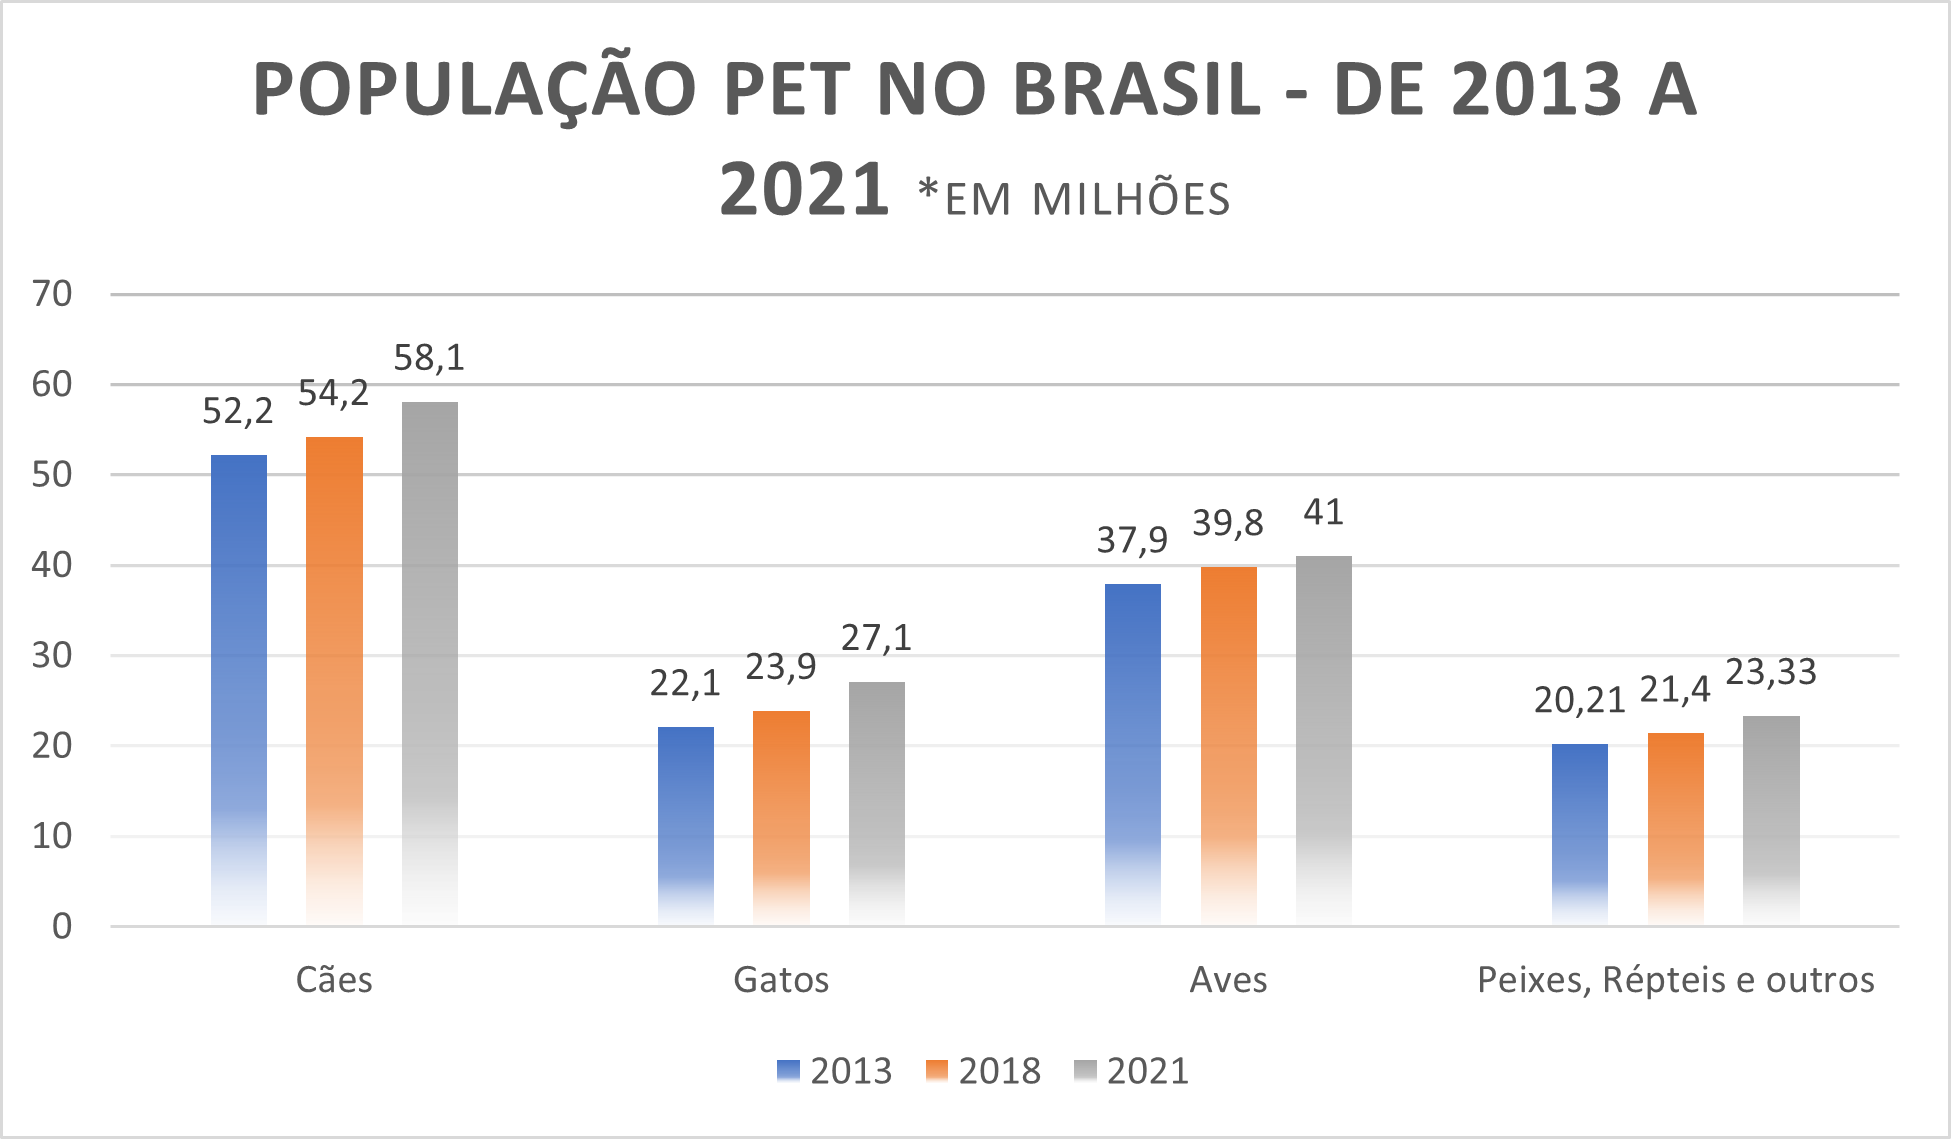
\includegraphics{images/grafico_censopet.png}
        \caption{Censo população Pet no Brasil, \citeonline{ibge2013, ibge2018, pet2021}}
        \label{fig:grafico_pet}
    \end{figure}

    \section{Análise da situação atual} \label{analise_atual}
    
    O documento obrigatório de maior valor durante o atendimento realizado pelo médico veterinário é, sem dúvidas, o prontuário veterinário. Atualmente são utilizados tanto versões físicas quanto versões digitais, ou eletrônicas, dos prontuários.
    
    Os prontuários eletrônicos são oferecidos por diversos sistemas de gerenciamento de clínicas veterinárias, por oferecerem armazenamento com acesso fácil aos dados dos prontuários, tendo em vista a declaração de João Abel Buck, médico-veterinário presidente da Associação Brasileira de Hospitais Veterinários (ABHV), fundada em 2017, por um grupo de empresários do segmento, em conversa com o CRMV-SP, onde garante que a transformação digital se apresenta de forma rápida, impulsionada pela pandemia que teve uma função catalisadora nisso, gerando uma grande necessidade do mercado de serviços veterinários em normatizar e regulamentar melhor este novo meio de se relacionar com os clientes utilizando da tecnologia como aliada \cite{buck}. Apesar da fidelidade das versões virtuais, os dados armazenados não podem substituir documentos físicos em eventos judiciais por não serem devidamente disciplinados por órgão regulamentador, nesse caso, pelos órgãos de classe que atestem a validade, \citeonline{pe_dig}, \citeonline{prontuario}.

    Além da questão regulatória, os sistemas de prontuários digitais atualmente disponíveis no mercado não torna os documentos imutáveis ou registram histórico de modificações. Assim, ao permitirem a alteração dos dados inseridos, sem permitirem consultar o histórico de alterações ou meios de rastreá-las, sujeita o estabelecimento ao risco de desamparo em caso de fiscalização por órgãos públicos ou perícias judiciais.
    
    Tendo em vista a dificuldade dos sistemas atuais de dar apoio em caso de fiscalizações e a premissa da existência de arquivos físicos, torna-se necessário manter os registros físicos em pastas-fichários após serem carimbados e assinados pelo médico veterinário, \citeonline{pe_dig}.
    
    O gerenciamento dos medicamentos controlados é realizado através de anotações manuais em um livro de registro. Esses registros devem ser realizados periodicamente e com exatidão pelo profissional veterinário, orientando e definindo os procedimentos a serem adotados dentro da clínica, a fim de prevenir descumprimentos das orientações. No entanto, demandam reserva de tempo e atenção para a execução de alguns desses procedimentos, como a operação de cálculos manuais para cada valor ou a repetição de anotações de mesmos dados em diferentes documentos, podendo interferir na performance e exigindo mais esforço do profissional, \citeonline{normativa}.
    
    Além das pontos fracos supracitadas, o armazenamento desses arquivos ocupa espaço físico e estão sujeitos a danos e perdas por mau armazenamento, como incidentes gerados por umidade, fogo, roubos e etc. O preenchimento desses dados em versões físicas e depois transcritos para versões digitais, pode ser um processo demorado e é sujeito a falhas, demandando um tempo que poderia ser melhor aplicado pelos profissionais envolvidos. Além disso, torna-se necessário um grau elevado de organização por parte da clínica, de tal modo que não prejudique que a consulta aos arquivos seja possível de forma a facilitar o serviço do profissional, \citeonline{pe_dig}.

    \section{Objetivos} \label{objetivos}

    A área de medicina veterinária ainda hoje opera de forma conservadora devido às suas necessidades burocráticas. E, por mais que o mercado ofereça algumas aplicações que têm a finalidade de automatizar o serviço, é difícil encontrar uma opção que ofereça funcionalidades que cumpram completamente as necessidades dos profissionais. Um dos motivos é que as soluções não são focadas em procedimentos específicos da veterinária, dividindo a ferramenta da aplicação com a gestão de Pet Shop.
    
    A aplicação, chamada de CertVet, tem como objetivo cobrir as principais necessidades de atuação do médico veterinário, automatizando os processos operacionais de atendimento e documentações clínicas, que hoje ainda demandam esforços manuais, garantindo o cumprimento de normas legais e regulamentares e propôr um fluxo do trabalho eficiente, diminuindo o tempo gasto neste, tendo em vista a observação da médica-veterinária, Mitika Kuribayashi Hagiwara, conselheira efetiva do CRMV-SP, professora sênior do Departamento de Clínica Médica e pesquisadora responsável pelo Grupo de Pesquisa em Patologia Clínica Veterinária, ambas da Faculdade de Medicina Veterinária e Zootecnia, da Universidade de São Paulo - FMVZ-USP, ao garantir em entrevista ao CRMV-SP que a necessidade de inserir informações dos animais atendidos por veterinários nos prontuários e em fichas clínicas de forma manual, demandava considerável espaço físico e muito mais tempo para busca e atualização dos dados, principalmente, em hospitais ou clínicas, onde há uma excessiva carga de serviços \cite{mitika}, sendo parte do escopo da CertVet, mitigar as problemáticas apontadas pela profissional, a fim de melhorar o desempenho do médico-veterinário, do atendimento e, consequentemente, da clínica.


    \section{Justificativa}\label{justificativa}

    Assim como o número de animais de companhia cresce a cada ano, a quantidade de profissionais veterinários atuantes no mercado brasileiro também apresenta crescimento, com 164.549 médicos veterinários inscritos de acordo com a contabilização do órgão federal, indicado na Figura \ref{fig:grafico vet}, \citeonline{vets_SP, vets2020, vets2022}.
    
    \begin{figure}[H]
        \centering
        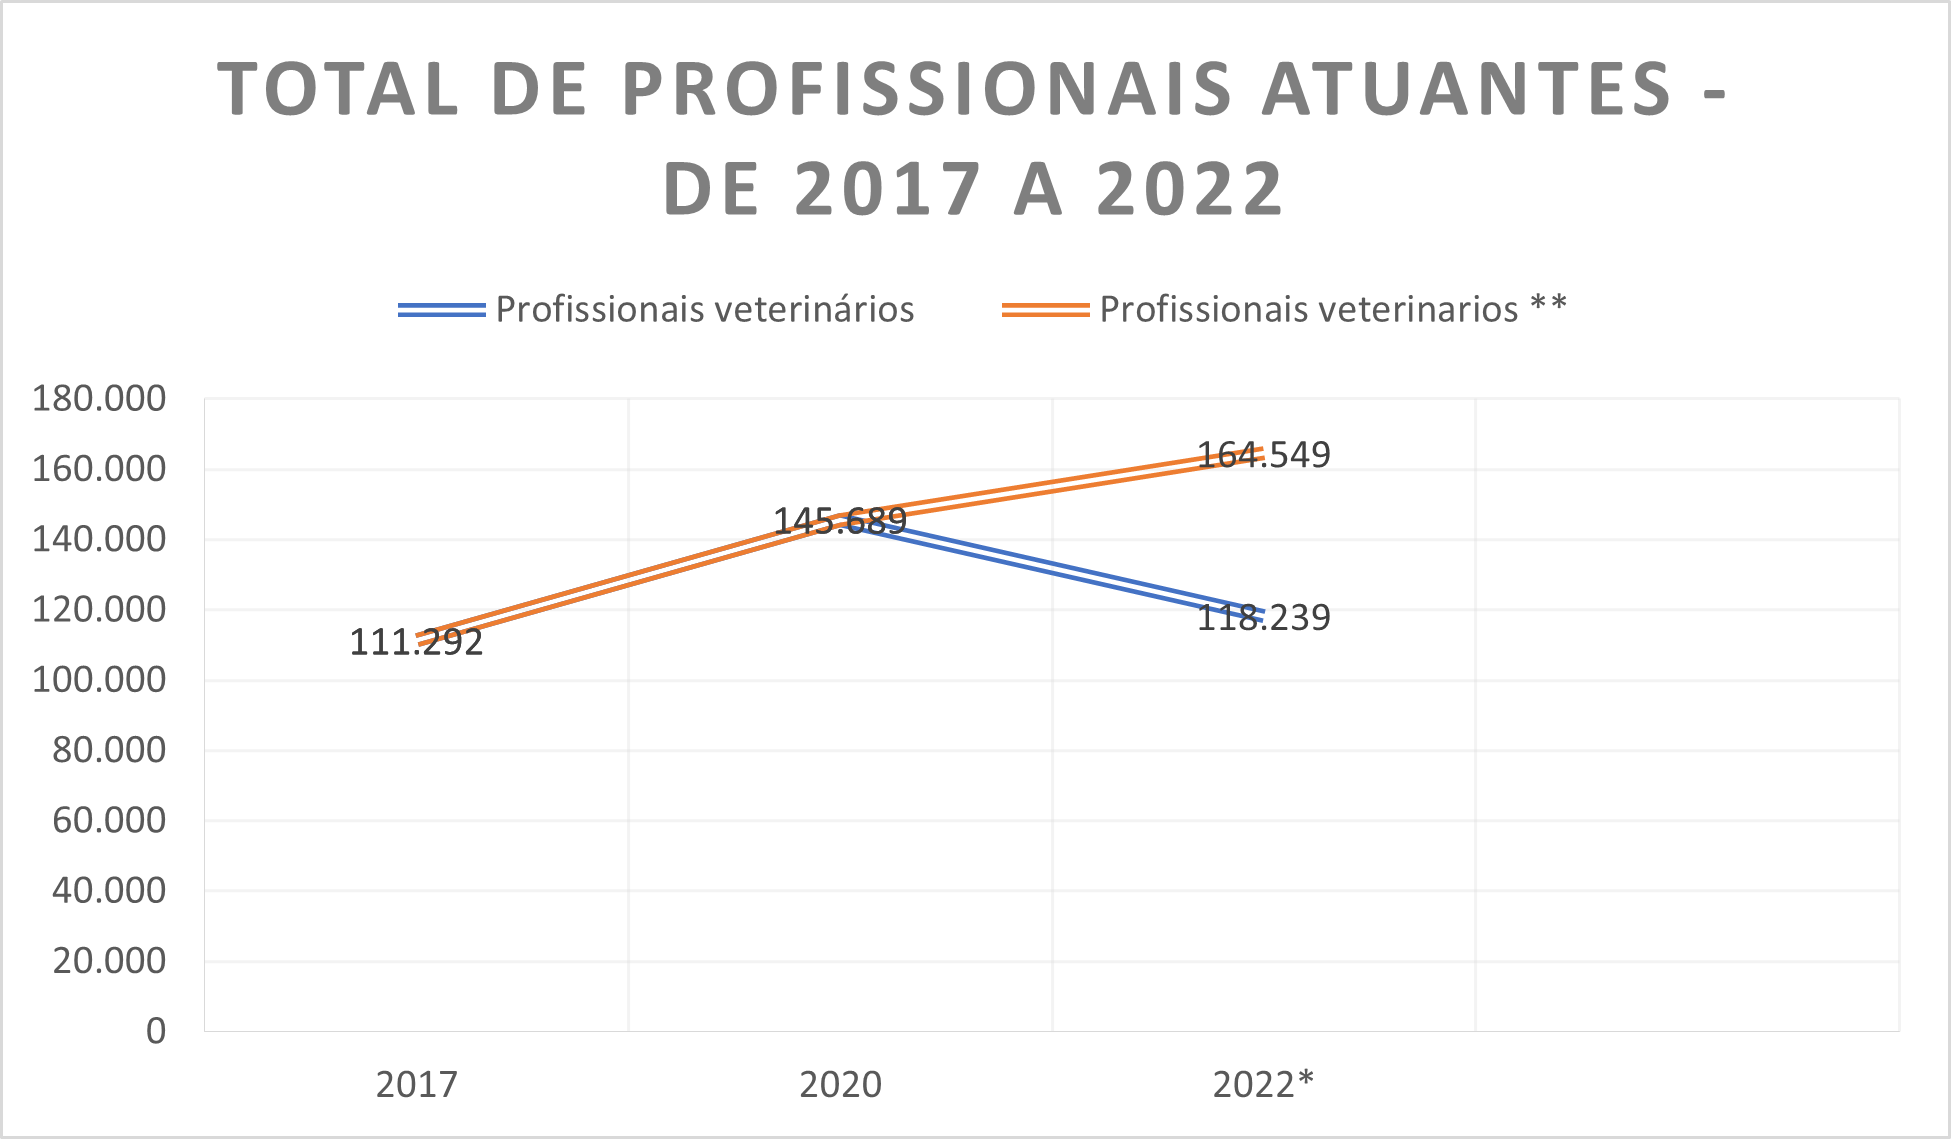
\includegraphics{images/grafico_profissionais.png}
        \caption{Número de veterinários registrados. *Dados sem os inscritos no Estado de São Paulo. ** Dados incluindo os inscritos no Estado de São Paulo.}
        \footnotesize {Fonte: \citeonline{vets2020,vets2022} }
        \label{fig:grafico vet}
    \end{figure}
    
    De acordo com o censo divulgado pelo CFMV para o biênio 2021/2022, atualmente existem 46.947 registros ativos de estabelecimentos veterinários, sendo divididos entre clínicas, hospitais, consultórios e ambulatórios, como podemos ver na Figura \ref{fig:grafico clinicas} \citeonline{clinicas2022}
    
    \begin{figure}[H]
        \centering
        \caption{Censo estabelecimentos veterinários no biênio 2021/2022}
        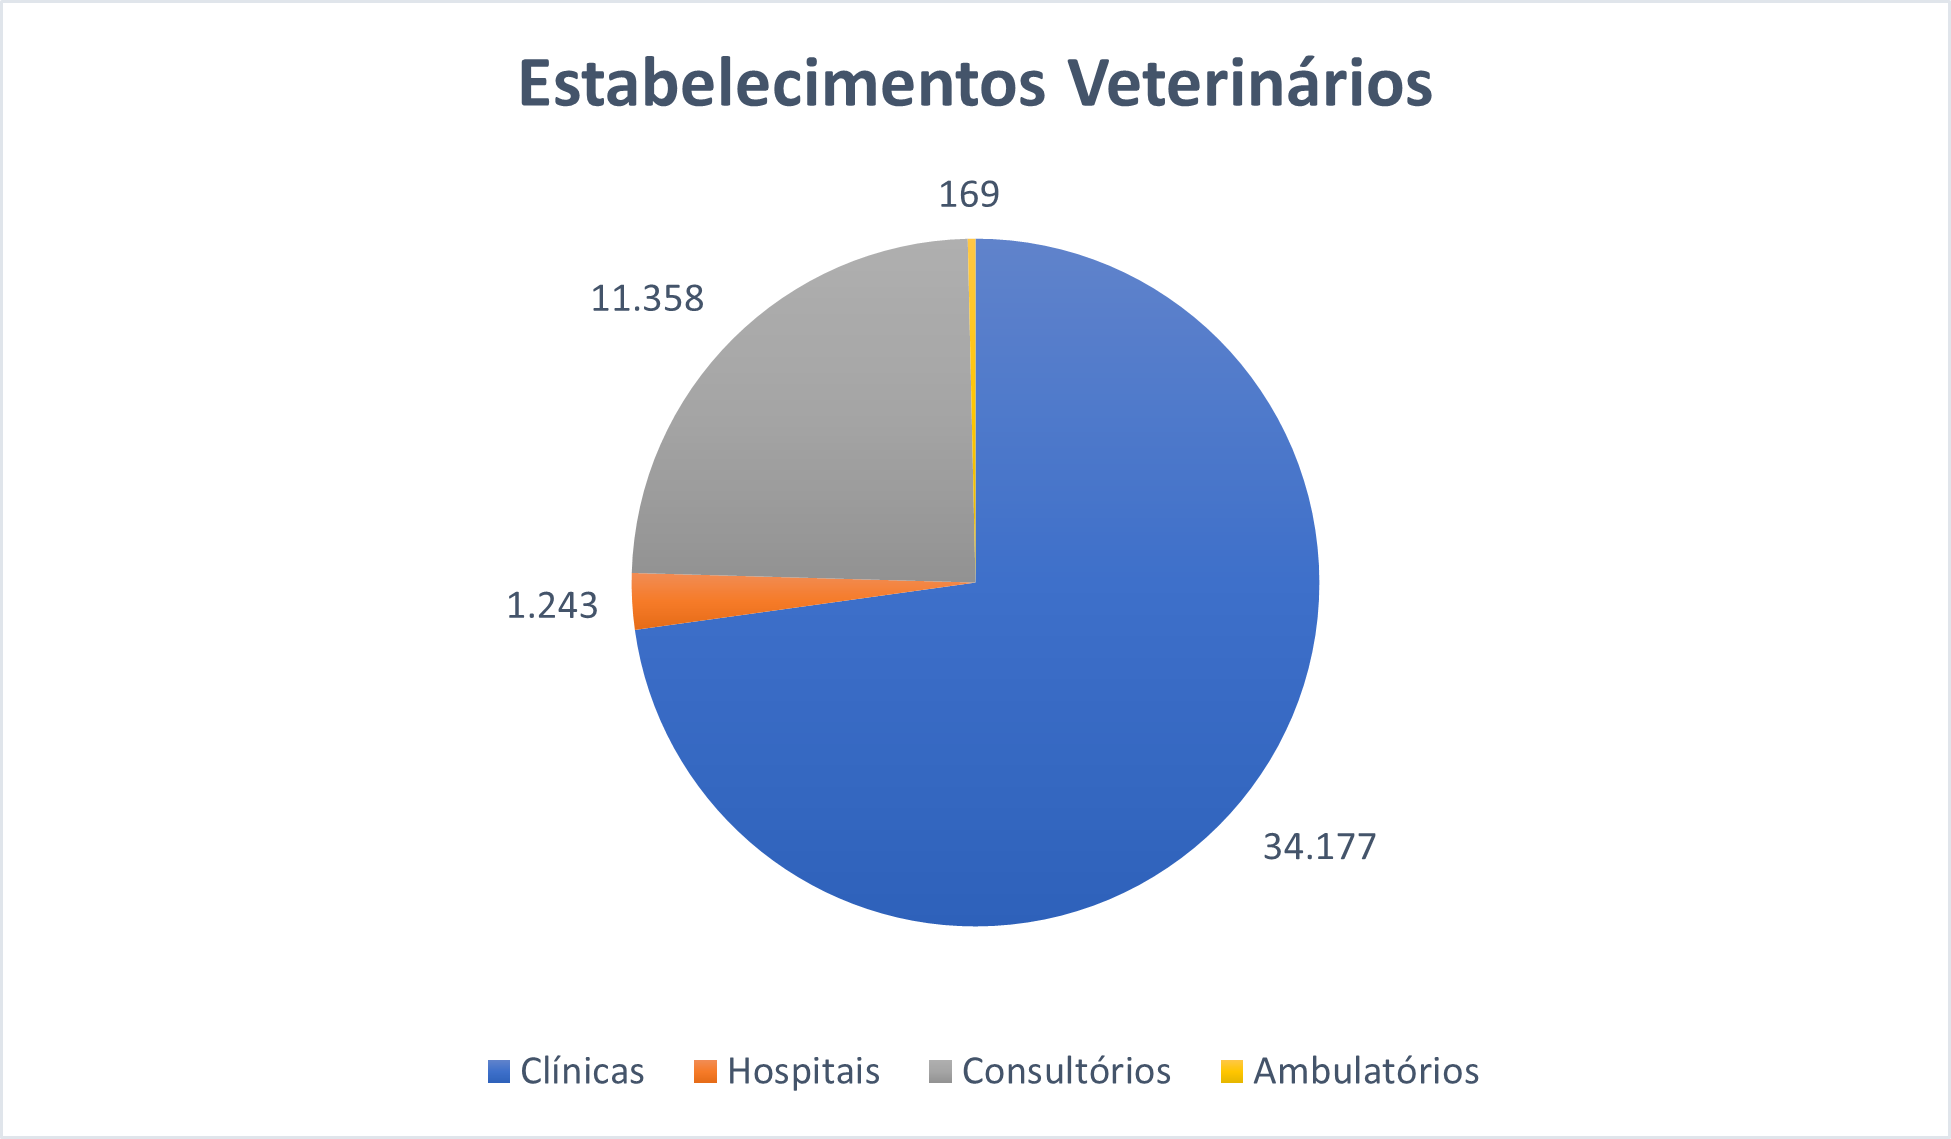
\includegraphics{images/grafico_estabelecimento.png}
        \footnotesize{ Fonte: \citeonline{clinicas2022}}
        \label{fig:grafico clinicas}
    \end{figure}
    
    Todos esses profissionais e estabelecimentos são fiscalizados e disciplinados pelas regras de conduta dos sistemas CFMV/CRMVs.
    
    Visando oferecer funcionalidades que permitam uma dinamização de todo o fluxo de trabalho do profissional veterinário, reduzir o tempo gasto com operações manuais, evitar a necessidades de anotações de informações repetidamente e reduzir o risco de erros de transcrição nas documentações, a CertVet consiste em um sistema que gerencia documentos com potencial valor legal e seus processos que se fazem necessários no fluxo de trabalho da medicina veterinária.
    
    Os processos automatizados agilizam os procedimentos fiscalizatórios e permitem que as alterações feitas sejam rastreadas, como é exigida pelo CFMV e pelos CRMVs \citeonline{teleMV}.
    
    A tecnologia da informação está modernizando a rotina de trabalho em áreas como automações de escritório, farmacêuticas e na medicina humana em estágios bem mais avançados que em relação ao atualmente aplicado na medicina veterinária. Compreende-se que existe a oportunidade de propor ritmo mais acelerado, garantindo a legalidade dos processos dentro de uma clínica veterinária.
    
    A partir das verificações de ambiente, referencial regulatório e constatação da situação, verificamos a necessidade do desenvolvimento de uma aplicação focada na automação de processos operacionais que otimizando o tempo de execução das tarefas do profissional veterinário e confiabilidade dos registros inseridos.
    
    Em pesquisa bibliográfica, não foram identificados fatos referentes à quantidade de profissionais ou estabelecimentos que utilizam algum sistema eletrônico ou de gestão. Porém, os meios de comunicação comumente enfatizam o crescimento de relevância econômica de serviços para o mercado de animais de estimação ano a ano. O sistema CertVet tem potencial para crescer e se destacar entre os demais sistemas já existentes.

    \section{Análise de Concorrência} \label{analise_concorrência}

        Nos últimos anos ocorreu modernização na dinâmica que rege a profissão do médico veterinário tanto pelo CFMV, como por seus órgãos regionais \citeonline{art_digital} \citeonline{cart_digital}, possibilitando que documentos obrigatoriamente físicos pudessem ser registrados em versões digitais válidos em todo território nacional. 
        
        A solicitação de tais documentos também pode ser realizada via navegação humana por sistema \emph{web} disponibilizado publicamente pelo CFMV, utilizando meios de identificação e autenticação nos sistemas regentes \citeonline{art_digital}. Este mesmo dado também pode ser utilizado por interface de aplicação, uma vez liberado por usuário habilitado por intermédio do CFMV.
    
        Para fins de comparação, foram selecionadas seis aplicações, já populares no mercado, que atuam na mesma problemática da CertVet.

\subsection{SimplesVet}
O SimplesVet se apresenta como um sistema para petshop e clínica veterinária que busca ajudar a simplificar a rotina da clínica \citeonline{simplesvet}. Consiste em um sistema acessado via \emph{web}, permitindo o controle da clínica a qualquer hora ou lugar, contanto que tenha acesso a internet. Suas funcionalidades dividem-se em:

\begin{itemize}
    
    \item Atendimento veterinário: permite o registro das fichas veterinárias em uma tela simples, com dados salvos na nuvem.
    \item Agenda de serviços: possibilita a organização da agenda dos veterinários e envia lembretes sobre os próximos atendimentos.
    \item Internação veterinária: organização dos prontuários e agendas de plantão.
    \item Controle financeiro: possibilita a organização do fluxo de caixa da clínica e envia lembretes de contas a pagar no celular cadastrado.
    \item Gestão de estoque: visualização dos produtos a repor, itens próximos ao vencimento, produtos parados e etc.
    \item Análise de vendas: visualização de um dashboard voltado à estratégias de marketing, listando produtos mais vendidos, ticket médio, horários de pico e etc.
    \item Notas fiscais: emissão de nota fiscal de consumidor eletrônica (NFC-e), nota fiscal de serviços eletrônica (NFS-e) e nota fiscal eletrônica (NF-e).
    \item \emph{App} para tutores: um \emph{app} feito para o cliente com datas de vacinação, exames e informações do pet.
    \item Mensagens automáticas: envio de lembrete de consultas e vacinas para os tutores e agenda para veterinários.
    \item \emph{Short Message Service (SMS) Marketing}: envio de campanhas via mensagens de texto para os clientes.
    \item Pesquisa e satisfação: possibilita o recebimento de avaliações dos clientes para fins comparativos com o mercado.
\end{itemize}

A SimplesVet possui mais \emph{features} voltadas à gerência de assuntos de \emph{PetShop}, como controle de estoque e de vendas, cumprindo de forma básica apenas uma das demandas da clínica veterinária \citeonline{simplesvet}. Enquanto a Certvet tem como principal objetivo resolver de forma simples as demandas do ambiente clínico, voltadas principalmente ao trabalho realizado pelo veterinário, como: manutenção de prontuário digital, controle de internação, controle da medicação e da autenticação de receitas, dentre outras, resolvendo demandas que não são contempladas pelo SimplesVet.

\subsection{Vetwork}
O Vetwork destaca-se entre os usuários pela sua interface intuitiva sendo algo que auxilia na produtividade do trabalho, trata-se de um sistema de gestão baseado na nuvem, não sendo necessária a instalação de hardware ou software, pois funciona nativo como \emph{Software as a Service (SaaS)} \citeonline{vetwork}. Seus 2.744 usuários dispõem das seguintes funcionalidades:

\begin{itemize}
    \item Agenda vinculada ao caixa: um controle geral das atividades realizadas nos \emph{pets}, como consultas médicas, retornos, exames, cirurgias, banhos, tosas e todos os outros procedimentos, sem limite de datas.
    \item Gestão de Documentos: permite a inclusão de documentos e arquivos à ficha clínica do animal, como laudos, fotografias, exames de imagem e outros, que são armazenados na internet e podem ser acessados de qualquer lugar.
    \item Calendário: uma forma de controle das datas e horários em que os animais passaram por procedimentos como banhos, tosas, exames, consultas, vacinas ou quaisquer outros realizados no estabelecimento.
    \item Gestão clínica: criação de prontuário eletrônico com as informações médicas do pet, como controle de registros clínicos, exames, vacinas e doses adicionais.
    \item Gestão Financeira: controle de caixa, pacotes, contas a pagar e a receber, pagamentos pendentes e pré-vendas, cálculo de comissionamento e geração de relatórios financeiros da empresa.
    \item Relacionamento com o Cliente: armazenamento de todas as informações dos clientes para possibilitar um relacionamento mais próximo com o mesmo.
    \item \emph{E-mail} Inclusos: mensagens automáticas, através de \emph{e-mail}, para comunicação instantânea.
\end{itemize}

Apesar de ser uma aplicação mais completa em relação à anterior, ainda assim o prontuário eletrônico é o ponto forte desse serviço, no que tange à funcionalidades para o fluxo clínico veterinário \citeonline{vetwork}. A CertVet busca resolver de forma eficaz e mais completa, o controle de medicamentos, não só o seu cadastro e quantidade em estoque, mas o uso de uma chave de autenticação para receitas e a aplicação dos mesmos. De forma resumida, o Vetwork é sim uma ferramenta bem útil mas a aplicação aqui proposta resolve demandas que não são resolvidas por esse serviço, por mais que suas avaliações no mercado sejam positivas.

\subsection{DoctorVet}
O DoctorVet é um sistema totalmente voltado à gestão de clínicas e hospitais veterinários e apresenta duas versões: uma \emph{Standard} com módulos para controle de consultas, vacinas, pequenas cirurgias, assuntos de pet shop e também financeiro. E uma versão enterprise que contempla todos os módulos \emph{Standard} e adicionalmente um controle de internação e hospedagem e concentra informações do centro cirúrgico e laboratório \citeonline{doctorvet}.  Funcionalidades da versão \emph{Enterprise} do DoctorVet:

\begin{itemize}
    \item Módulo de Cadastro: realiza o cadastro de veterinários, funcionários, animais, clientes e planos de atendimento.
    \item Módulo Farmacológico: permite o cadastro de vacinas, vermífugos e o cadastro de procedimentos ou interações medicamentosas.
    \item Módulo Atendimento: criação de ficha de atendimento, lista de espera, curadoria de orçamentos, central de   agendamentos e controle de status do veterinário.
    \item Módulo Caixa: utilizado pelos atendentes de caixa, controle das formas de recebimento, abertura e fechamento do caixa e manutenção.
    \item Módulo Consultório: consultas generalistas e especialistas, histórico de consultas e atendimentos, pedidos de exames, receituários e prontuário eletrônico.
    \item Módulo Pet Shop: permite televendas, consulta de preços e relatórios e emissão de cupom fiscal.
    \item Módulo Internação Básica/Avançada: admissão de internação, controle da evolução do quadro clínico, alta veterinária, manter prontuários, cadastro de prescrições.
    \item Módulo Estoque: cadastro de fornecedores, cadastro e etiquetação de produtos, gerenciamento de lotes, requisições à farmácia e requisições internas, controle de compras e relatórios.
    \item Módulo Exames: controle de exames laboratoriais e seus resultados.
    \item Módulo Laboratório: cadastros, central de coleta e composição de exames.
    \item Módulo Centro Diagnóstico: preparo para exames e suas composições.
    \item Módulo Relatórios: criação de relatórios operacionais, gerenciais e estratégicos em concordância com Gestão de Relacionamento com o Cliente (CRM), Sistema Público de Escrituração Digital Fiscal (SPED), Programa de Integração Social (PIS) e Contribuição para o Financiamento da Seguridade Social (Cofins).
    \item Módulo Segurança: cadastro de usuários e permissões de acesso de acordo com níveis.
\end{itemize}

É a aplicação mais recente das selecionadas e também a mais completa, no entanto, reforça-se aqui que não contempla o controle de medicamentos \citeonline{doctorvet}, oferecido pela Certvet.

\subsection{Dr. Snoopy Smart}
O Dr. Snoopy Smart se apresenta como um sistema completo de gestão exclusivo para Pet Shop e clínicas veterinárias, automatizando processos clínicos, na tentativa de agilizar as tarefas e tendo o aumento das vendas como foco do módulo de pet shop \citeonline{drsnoopy}. Consiste em um software com as seguintes funcionalidades:

\begin{itemize}
    \item Agendamento otimizado: permitindo o controle de agendamento dos pacientes.
    \item Gerenciamento de estoque: visibilidade da quantidade de produtos e quais estão em falta.
    \item Prontuário Clínico: possibilita a criação e consulta da ficha veterinária dos animais.
    \item Emissão de Notas: emissão de nota fiscal eletrônica (NF-e), nota fiscal de serviços eletrônica (NFS-e) e cupons fiscais.
    \item Histórico de Pacientes: arquivação e consulta de informações dos atendimentos. 
    \item Vacinas sempre em dia: controle de quando o paciente deve ser vacinado.
    \item Agenda de Banho e Tosa: específica para tais, permitindo um maior controle do pet shop.
    \item Gestão Integrada: permite acessar à determinados indicadores de gestão.
    \item Notificações \emph{Short Message Service} (SMS): recebimento de lembretes importantes no celular dos usuários da aplicação
    \item Relatórios Personalizados: geração de relatórios com facilidade.
\end{itemize}

Apesar de ser uma aplicação com muitas funcionalidades, ainda assim não apresenta as opções de modernidade que a aplicação aqui proposta oferece, considerando-se que divide o escopo clínico com as necessidades de um pet shop, apresentando mais funcionalidades voltadas à gestão e estratégias de venda do que para o fluxo de trabalho do profissional veterinário.

\subsection{Vetsoft}
O programa VetSoft é oferecido nas versões \emph{Desktop} e \emph{Web}, sendo essa primeira uma versão instalada nos computadores em rede, permitindo o acesso mesmo com falta de conexão com a \emph{internet}. E a versão \emph{Web}, um sistema em nuvem que permite ao usuário gerenciar o negócio através de diferentes dispositivos, seja pelo computador ou pelo \emph{smartphone}, contanto que tenha acesso à internet \citeonline{vetsoft}. O VetSoft abrange serviços de clínica veterinária, hospital veterinário, \emph{pet shop} / banho e tosa e veterinários autônomos com as seguintes funcionalidades:

\begin{itemize}
    \item Ficha do Tutor: ficha cadastral da conta do tutor e seus animais, visibilidade do histórico de pagamentos e envio de e-mail individual.
    \item Ficha do Animal: ficha cadastral específica dos animais pacientes, álbum de fotos, agendamentos, agrupamento dos resultados de exames e histórico de vacinas e vermífugos.
    \item Histórico Clínico: anamnese, diagnóstico, laudo clínico, receituário normal e especial e exames.
    \item Gestão de Estoque: divisão de produtos por grupos, controle de produtos com estoque baixo, visibilidade dos produtos mais e menos vendidos e entrada de estoque manual e XML.
    \item Financeiro: controle de caixa diário e seu fluxo, demonstrativo de resultados por área, centro de custos, controle de planos para clientes mensalistas.
    \item Emissão Fiscal: possibilidade de emissão fiscal para todos os estados e os formatos: Nota Fiscal de Consumidor Eletrônica (NFCe), Sistema Autenticador e Transmissor de Cupons Fiscais Eletrônicos (SAT), Módulo Fiscal Eletrônico (MFe) e Programa Aplicativo Fiscal – Emissor de Cupom Fiscal (PAF-ECF).
    \item Farmácia/Materiais: controle de estoque de farmácia e materiais de uso interno.
    \item Imunizações: controle da aplicação de vacinas e vermífugos na ficha do animal com agendamentos e aplicações realizadas.
\end{itemize}

É uma das aplicações mais completas, no entanto, o controle de medicamentos oferecido não atinge o mesmo grau de segurança que a chave de autenticação para as receitas que a CertVet oferece, assumindo um papel importante na modernização dessa autenticação nos dias atuais.

\subsection{BensVet}
O BensVet se diferencia dos demais apresentados por se tratar de um serviço que se divide em dois aplicativos, um para uso veterinário e um para uso dos tutores. O aplicativo para veterinários garante que o usuário poderá iniciar um atendimento a domicílio e conseguir  dar continuidade na clínica. E o aplicativo para tutores trata-se dos processos de envio  de promoções e alertas de retorno automáticos para os tutores, permitindo também a consulta de  informações sobre o animal e agendamento de atendimentos pelo \emph{App},  \citeonline{bensvet}. As funcionalidades dividem-se em:

\begin{itemize}
    \item Agenda de atendimentos.
    \item Acompanhamento de medicações na internação.
    \item Criação de fichas clínicas personalizadas.
    \item Notificar automaticamente consultas, retornos e vacinas aos clientes.
    \item Consultar históricos de animais e seus tutores.
    \item Controle dos comissionamentos de profissionais.
    \item Emitir Notas Fiscais referente a venda de produtos.
    \item Controle de estoque.
\end{itemize}

Trata-se de uma resolução que se aproxima bastante da CertVet no que tange à proximidade do profissional veterinário, esteja ele numa clínica ou trabalhando de forma autônoma, no entanto, observamos aqui que o controle de medicamentos oferecido, mais uma vez, não atinge o mesmo grau de segurança que a chave de autenticação aqui propostas, além da funcionalidade de consulta ao histórico de aspectos hereditários.

\subsection{Quadro comparativo de concorrentes}
Com base no levantamento acima, foi possível observar algumas intersecções das funcionalidades oferecidas. O Quadro \ref{tab:comparativa} permite melhor visualização deste levantamento.

\begin{center}
    \begin{quadro}[H]
     \caption{Comparação das aplicações concorrentes}
    \label{tab:comparativa}
    \begin{tabulary}{1.0\textwidth}{|L|L|L|L|L|L|L|L|L|}
    \hline
     & CertVet & Simples Vet & Vet work & Doctor Vet & Dr. Snoopy Smart & Vet soft & Beans Vet\\
    \hline
    Agenda & x & x & x & x & x & x & x\\
    \hline
    Prontuário clínico & x & x & x & x & x & x & x\\
    \hline
    Gerenciamento de medicação & x & x &  & x & x & x & x\\
    \hline
    Controle de vacina\c{c}ão & x &  &  & x & x & x & x\\
    \hline
    Histórico de Aspectos Hereditários & x &  &  &  &  &  & \\
    \hline
    Rastreio de alterações & x &  &  &  &  &  & \\
    \hline
    Gestão Financeira &  & x & x & x & x & x & x\\
    \hline
    Gestão PetShop &  & x & x & x & x & x & x\\
    \hline
    \end{tabulary}
    \centering
    {\footnotesize Fonte: Elaborado pelos autores.}
    \end{quadro}
\end{center}

\chapter[Revisão de Literatura]{Revisão da Literatura} \label{revisao_lit}

    Este capítulo aborda uma breve revisão bibliográfica sobre a documentação obrigatória emitida por estabelecimentos veterinários, revisão das leis referentes a tais documentos, novos caminhos abordados pelo Conselho Federal de Medicina Veterinária e como esse aspectos são relevantes ao nosso projeto.


    \section{Documentação Obrigatória e Legislação Pertinente}
    
        De acordo com a Resolução nº1321, de 24 de abril de 2020 \citeonline {doc_obrig}, todo estabelecimento veterinário e/ou médico veterinário deve emitir documentos específicos no âmbito de suas respectivas atividades profissionais.
        
        Tais documentos, de caráter obrigatório, deve seguir os padrões estabelecidos pelo Conselho Federal de Medicina Veterinária, que regulamenta a profissão do médico veterinário, de acordo com a Lei nº 5.517, alínea “f”, do artigo 16, de 23 de outubro de 1968. \citeonline {doc_obrig}.
        
        A Resolução 1321/2020, em seu Art. 2º, define o prontuário veterinário como \citeonline {doc_obrig}: 
    
        \begin{citacao}
            
        
            VIII - prontuário médico-veterinário: documento escrito e datado, sem rasuras ou emendas, emitido e assinado, privativamente por médico-veterinário que relata e detalha, cronologicamente, informações e dados acerca dos atendimentos ambulatoriais e clínicos, inclusive vacinações, exames diagnósticos e intervenções cirúrgicas realizados em animal, ou coletivo em se tratando de rebanho, garantida a autenticidade e integridade das informações;
        \end{citacao}
    
        Outros documentos obrigatórios estão dispostos no Quadros \ref{doc_obrigatorio_demanda}, \ref{doc_obrigatorio_demanda2} e \ref{quad:documentos3}: 
    
\begin{center}
    \begin{quadro}[H]
    \caption{Relação de Documentos de Caratér Obrigatórios e Demanda}
    \label{doc_obrigatorio_demanda}
    \begin{tabulary}{1.0\textwidth}{|p{10em}|p{15em}|p{10em}|}
    \hline
    Nome & Objetivo do documento & Obrigatoriedade\\
    \hline
    Atestado ou declaração de óbito (Anexo \ref{atestado de obito}) & Documento escrito e datado, sem rasuras ou emendas, emitido e assinado, privativamente, por um médico-veterinário para declarar o óbito do animal e a provável causa mortis & Não, disponível sob demanda\\
    \hline
    Atestado ou declaração de vacinação (Anexo \ref{atestado de vacina}) & Documento escrito e datado emitido e assinado, privativamente, por um médico-veterinário para declarar o ato vacinal com a devida identificação do animal vacinado & Sim, quando houver necessidade de ato vacinal\\
    \hline
    Atestado sanitário (Anexo \ref{atestado sanitario}) & Documento escrito, sem rasuras ou emendas, datado, emitido e assinado privativamente por um médico-veterinário para declarar o estado ou condições de saúde do(s) animal(is) & Não, disponível sob demanda\\
    \hline
    Prontuário médico-veterinário (Anexo \ref{atestado de obito}) & Documento escrito e datado, sem rasuras ou emendas, emitido e assinado, privativamente por um médico-veterinário que relata e detalha, cronologicamente, informações e dados sobre os atendimentos ambulatoriais e clínicos, inclusive vacinações, exames diagnósticos e intervenções cirúrgicas realizados em animal, ou coletivo em se tratando de rebanho & Sim, em todo atendimento clínico veterinário\\
    \hline
    Termo de consentimento livre esclarecido para realização de exames (Anexo \ref{consentimento exame}) & Documento a ser apresentado por médico-veterinário para assinatura do responsável pelo animal com o objetivo de formalizar a ciência e livre consentimento ou autorização para realização de exames veterinários & Sim, quando houver necessidade de realizar exame(s)\\
    \hline
    Termo de consentimento livre esclarecido para realização de procedimentos terapêuticos de risco ou experimental (Anexo \ref{consentimento tratamento}) & Documento a ser apresentado por médico-veterinário para assinatura do responsável pelo animal com o objetivo de formalizar a ciência e livre consentimento ou autorização para realização de procedimento terapêutico que tenha elevado grau de comprometimento ou perda de sentido ou função, debilidade ou deformidade, bem como óbito & Sim, quando houver necessidade de realizar procedimento(s) terapêutico(s)\\
    \hline
    \end{tabulary}
    \centering
    \footnotesize {Fonte: \citeonline{doc_obrig}}
    \end{quadro}
\end{center}
    
\begin{center}
    \begin{quadro}[H]
    \caption{Relação de Documentos de Caratér Obrigatórios e Demanda - continuação }
    \begin{tabulary}{1.0\textwidth}{|p{10em}|p{15em}|p{10em}|}
    \hline
    Nome & Objetivo do documento & Obrigatoriedade\\
    \hline    
    Termo de consentimento livre esclarecido para retirada de corpo de animal em óbito (Anexo \ref{retirar corpo}) & Documento a ser apresentado por médico-veterinário para assinatura do responsável pelo animal com o objetivo de esclarecer e transferir a esse a responsabilidade pela posse e destinação ambiental adequada do cadáver & Não, disponível sob demanda\\
    \hline
    Termo de consentimento livre esclarecido para realização de procedimento cirúrgico (Anexo \ref{consentimento cirurgico}) & Documento a ser apresentado por médico-veterinário para assinatura do responsável pelo animal com o objetivo de formalizar a ciência e livre consentimento ou autorização para realização de procedimento cirúrgico & Sim, quando houver necessidade de realizar procedimento(s) cirúrgico(s)\\
    \hline
    Termo de consentimento livre esclarecido para realização de procedimento anestésico (Anexo \ref{consentimento anestesico}) & Documento a ser apresentado por médico-veterinário para assinatura do responsável pelo animal com o objetivo de formalizar a ciência e livre consentimento ou autorização para realização de procedimentos de anestesia & Sim, quando houver necessidade de realizar procedimento(s) cirúrgico(s)\\
    \hline
    Termo de consentimento livre esclarecido para internação e tratamento clínico ou pós-cirúrgico (Anexo \ref{consentimento internacao}) & Documento a ser apresentado por médico-veterinário para assinatura do responsável pelo animal com o objetivo de formalizar a ciência e livre consentimento ou autorização para realização de internação e tratamento clínico ou pós-cirúrgico & Sim, quando houver necessidade de internação e tratamento clínico ou pós-cirúrgico\\
    \hline
    Termo de consentimento livre esclarecido para realização de eutanásia (Anexo \ref{consentimento eutanasia}) & Documento a ser apresentado por médico-veterinário para assinatura do responsável pelo animal com o objetivo de formalizar a ciência e livre consentimento ou autorização para realização de eutanásia no animal & Não, disponível sob demanda\\
    \hline
    \end{tabulary}   
    \label{doc_obrigatorio_demanda2}
    \centering
    \footnotesize {Fonte: \citeonline{doc_obrig}}
    \end{quadro}
\end{center}


%%%%%%%%%%%%%%%%%%%%%%

\begin{center}

    \begin{quadro}[H]
    \caption{Relação de Documentos Obrigatórios e Demanda - continuação}
    \begin{tabulary}{1.0\textwidth}{|p{10em}|p{15em}|p{10em}|}
    \hline
    Nome & Objetivo do documento & Obrigatoriedade\\
    \hline
    Termo de consentimento livre esclarecido para retirada do serviço veterinário sem alta médica (Anexo \ref{retirada sem alta}) & Documento a ser apresentado por médico-veterinário para assinatura do responsável pelo animal com o objetivo de esclarecimento e obtenção da manifestação de livre intenção de retirada do animal de serviço veterinário sem alta médica, bem como de assunção de plena e irrestrita responsabilidade sobre os riscos sanitários e de morte do animal & Não, disponível sob demanda\\
    \hline   
    Termo de consentimento livre esclarecido para doação de corpo de animal para ensino e pesquisa (Anexo \ref{doacao de corpo}) & Documento a ser apresentado por médico-veterinário para assinatura do responsável pelo animal com o objetivo de esclarecimento e obtenção da manifestação de livre doação do corpo do animal para encaminhamento a instituição de ensino e pesquisa & Não, disponível sob demanda\\
    \hline
    Termo de consentimento livre esclarecido para realização de pesquisa clínica (Anexo \ref{atestado de obito}) & Documento a ser apresentado por médico-veterinário para assinatura do responsável pelo animal com o objetivo de esclarecimento e obtenção de autorização de submissão do animal a estudo ou pesquisa & Não, disponível sob demanda\\
    \hline
    \end{tabulary}   
    \label{quad:documentos3}
    \centering
    {\footnotesize Fonte: \citeonline{doc_obrig}}
    \end{quadro}
\end{center}
    
        Dentre as regras referidas na Resolução nº 1321 de 2020, seu artigo 3º disciplina dados para a composição do prontuário médico:
    
        \begin{citacao}
            
        
            Os documentos emitidos por médicos-veterinários comporão o prontuário do paciente (...) conter os seguintes dados e informações: nome completo e assinatura do médico-veterinário, número de inscrição no Sistema CFMV/CRMVs, endereço, telefone,\emph{e-mail} e, se for o caso, identificação do estabelecimento (razão social, CNPJ e número de registro no Sistema CFMV/CRMVs)
        \end{citacao}
    
        No inciso VI, especifica fatos relacionados ao animais que devem constar por observação física:
        
        \begin{citacao}
            
            (Deve) conter informações que permitam a identificação do paciente, tais como nome, sexo, raça, idade real ou presumida, cor de pelagem ou plumagem, sinais particulares, tatuagem, brinco, \emph{microchip}, registro genealógico e, conforme o caso, resenha detalhada;(...) identificação do responsável pelo animal (nome completo, CPF e endereço completo)
        \end{citacao}
    
        Em seu inciso VII, § 2º, dispõe sobre requisitos para operação de através de mídias virtuais: 
    
        \begin{citacao}
            Os documentos expedidos eletronicamente deverão contar com sistemas capazes de garantir a segurança, autenticidade, confidencialidade e integridade de informações, bem como o armazenamento e compartilhamento dos dados.
        \end{citacao}
    
        As regulamentações acima garantem a legitimidade do sistema proposto, pois servem de embasamento legal e diretrizes a serem seguidas.
        
        A autorização para se realizar a telemedicina na área veterinária também adere à tendência de modernização na profissão e viabiliza que soluções digitais sejam implementadas relativas a documentação obrigatória.\citeonline{teleMV}.
        
        Com relação à gestão de medicamentos controlados (de uso restrito e com retenção de receitas), de acordo com as leis vigentes da Instrução Normativa nº 35, de 11 de setembro de 2017, Capítulo I, Art. 2º, § IV, Capitulo IV, § 11  \citeonline{normativa}, ela é realizada através de um caderno de capa dura, no formato brochura, no qual o médico veterinário Responsável Técnico (RT) anota a data de entrada dos medicamentos no estoque e quanto desse medicamento foi utilizado no dia, para cada procedimento. Este caderno é denominado Livro-Registro.
        
        \section{Diferença entre Prontuário e Histórico Médico }

    De acordo com o Conselho Federal de Medicina (CFM), prontuário médico é um documento que apresenta todos os dados relativos ao paciente, como o histórico familiar, anamnese, descrição e evolução de sintomas e exames realizados por esse paciente, além de prescrições de tratamento a ser seguido. Esse documento tem como objetivo facilitar a assistência ao paciente. Embora feito durante o atendimento médico no consultório ou hospital, o paciente é considerado o proprietário desse registro podendo ter acesso e solicitar cópias, \citeonline{prontuario_medico}.


    Em contrapartida, o histórico médico é um documento cujo objetivo é registrar todas as informações relevantes do paciente sobre sua saúde, contribuindo dessa maneira para a análise completa do quadro de saúde do paciente por profissionais da saúde. Nesse documento deverão ser registrados não apenas o histórico de doenças, mas informações sobre consultas prévias que esse paciente teve durante a sua vida, \citeonline{historico_medico}, hábitos e doenças. Esse documento ajuda na prevenção de patologias, visto que esse sinaliza possíveis fatores de risco à saúde do paciente. %(https://telemedicinamorsch.com.br/blog/historico-do-paciente)

    A diferença entre histórico médico e prontuário, embora seja muito sutil, esta existe e consiste no fato de que o histórico médico apresenta um dados cronológicos sobre o paciente, ou seja, o que ele já teve e o que ele está tendo, enquanto o prontuário não faz relação com seu histórico, limitando-se a registrar as informações do paciente e de seu tratamento para uma determinada situação, \citeonline{prontuarioXhistorico}. 

\chapter[Metodologias]{Metodologias}

    O projeto propõe a criação de um sistema de gerenciamento de processos e documentação exigidas pelo órgão de classe veterinária, além de implementar funcionalidades já existentes em outros sistemas de gestão de estabelecimentos veterinários. 

    \section{Proposta}
    
        Tendo em vista os pontos fracos das soluções disponíveis atualmente, anteriormente mencionados no Capítulo \ref{objetivos}, a CertVet oferece a gestão das atividades do médico-veterinário, cobrindo o fornecimento de informações gerenciais de toda a clínica, como os cadastro de funcionários e clientes e as informações que se fazem necessárias. 
        
        No segmento de atendimento veterinário, a aplicação oferece o recurso de prontuário clínico digital, no qual permite a análise rápida de todo histórico assistencial dos animais, aplicando a assinatura eletrônica a esses arquivos, utilizando um certificado digital válido padrão ICP-Brasil, sendo esse o processo responsável por garantir a verificabilidade e rastreabilidade de alterações feitas, bem como os devidos registros de data e hora, sendo assim, passível de fiscalização.
        
        Complementarmente, para os registros de medicamentos controlados, é possível cruzar os dados movimentação de determinados medicamentos disponíveis no estoque, suas movimentações no livro-registro e valores desses medicamentos que estão sendo utilizados durante os procedimentos, atribuindo maior consistência aos registros e diminuindo o retrabalho de se adicionar as mesmas informações manualmente. O sistema realiza os cálculos de quantidade de medicamentos utilizados e atualiza-os no livro-registro digital.

    \section{Funcionalidades}
    
        Considerando as necessidades do dia a dia de um médico-veterinário, suas atividades dentro da clínica e partindo do estudo da concorrência, serão implementadas as seguintes funcionalidades:
    
        \begin{itemize}
            \item Cadastro de funcionários, tutores, animais e atendimentos, permitindo que o veterinário efetue o atendimento dispondo das informações necessárias centralizadas nas fichas cadastrais dos funcionários, tutores e animais.
            \item Assinatura digital, garantindo caráter legal aos documentos, tendo em vista que permite rastrear e verificar os responsáveis por alterações feitas no prontuário. 
            \item Gestão de estoque de medicamentos controlados, para que o responsável técnico informe a data de entrada do medicamento e o quanto deste foi utilizado no dia, cumprindo às normas do livro-registro \citeonline{normativa}.
            \item Validador de cadastro profissional para acessar área restrita do sistema, considerando que algumas atividades são de exclusiva responsabilidade de um profissional veterinário em atividade, como pode ser lido nos Quadros \ref{tab:req_func} e \ref{tab:hist_usuario}.
            \item Histórico de aspectos hereditários, permite que o veterinário faça as devidas anotações quando for observado casos de alergia ou intolerância a medicamentos que possuam aspectos genéticos e doenças que podem ser transmitidas geneticamente. Servindo de base para melhor atendimento de um animal que possua consanguinidade ou parentesco com o animal das observações.
        \end{itemize}
    
        \subsection{Funcionalidades Futuras}
            
            Algumas possíveis implementações de funcionalidades futuras são a importação e exportação dos dados entre estabelecimentos que utilizam o mesmo sistema, digitalização das notificações de aquisição de medicamentos controlados com a nota fiscal da compra do produto, automatizando a entrada desses dados no estoque e permitindo a fiscalização.
        
        \subsection{Possíveis Integrações e Parcerias}
        
        Para que seja possível a validação dos registros de profissionais veterinários ativos a serem registrados na plataforma, está sendo estudada a integração da CertVet com o Sistemas de Cadastros do Conselho Federal de Medicina Veterinária (SISCAD).
        
        Além de uma possível parceria com os órgãos responsáveis pela fiscalização regional de cada estado, os CRMVs.

    \section{Fluxo de Processos na Clínica Veterinária}

    A rotina da clínica veterinária é constituída de processos, que organizam a rotina do estabelecimento, assim como seus procedimentos. Podemos dizer que o cadastro de um cliente gera um fluxo de processo, relacionado a tal ação. A ordem em que um profissional realiza sua atividade, no caso do nosso projeto, realiza uma consulta ou atendimento veterinário, segue-se um fluxo de ações, numa ordem pre-estabelecida, por convenção, pelos profissionais da área. 

    Um fluxo de processo garante ordenamento e agilidade, padronizando o processo para que todos os profissionais da área, ou do estabelecimento, tenham uma conduta uniforme, visando atingir melhores resultados.

    Baseado na literatura e na experiência vivida pela integrante do grupo, foram elaborados os seguintes processos de cadastro e de atendimento de um animal, dentro de uma clínica, \citeonline{Rabelo:2012}.

    Ressalta-se que são processos do tipo \emph{AS-IS}, de um estabelecimento de médio porte, que nosso sistema CertVet pretende englobar na sua versão futura, se possível no produto final.
    
    \subsection{Contato Inicial - Necessidade de Atendimento}
    
     Neste fluxo um tutor necessita de atendimento para seu animal. Ele chega na recepção do estabelecimento e o seguinte processo é iniciado:
     
      - Tutor solicita atendimento à recepcionista do estabelecimento veterinário.
      
      - Recepcionista verifica se tutor possui cadastro em nome dele e também do seu animal.
      
      - Caso exista o cadastro, recepcionista verifica se existe o agendamento prévio. Se confirmado agendamento, informar ao tutor que animal será atendido em breve.
      
      - Caso não possui agendamento, verificar disponibilidade de horários e informar tutor.
      
      - Tutor escolhe horário e aguarda atendimento.
      
      - Caso não exista o cadastro do tutor ou do animal, recepcionista deve coletar os dados do tutor e animal para criar cadastro.
      
      - Após cadastro informar tutor da disponibilidade de horário.
      
      - Tutor escolhe horário e aguarda atendimento.

      
O fim do processo se dá com o animal sendo atendido pelo médico veterinário da clínica, caso o tutor tenha agendamento ou selecione um horário, ou o processo se encerra caso não exista horário disponível ou tutor não aceite os horários ofertados.

    %Na figura \ref{fluxo-rec} podemos ver o fluxo desse processo utilizando a notação BPMN.


    \begin{sidewaysfigure}[H]
        \centering
         \caption{Processo \emph{AS-IS} do Atendimento - Recepção}
        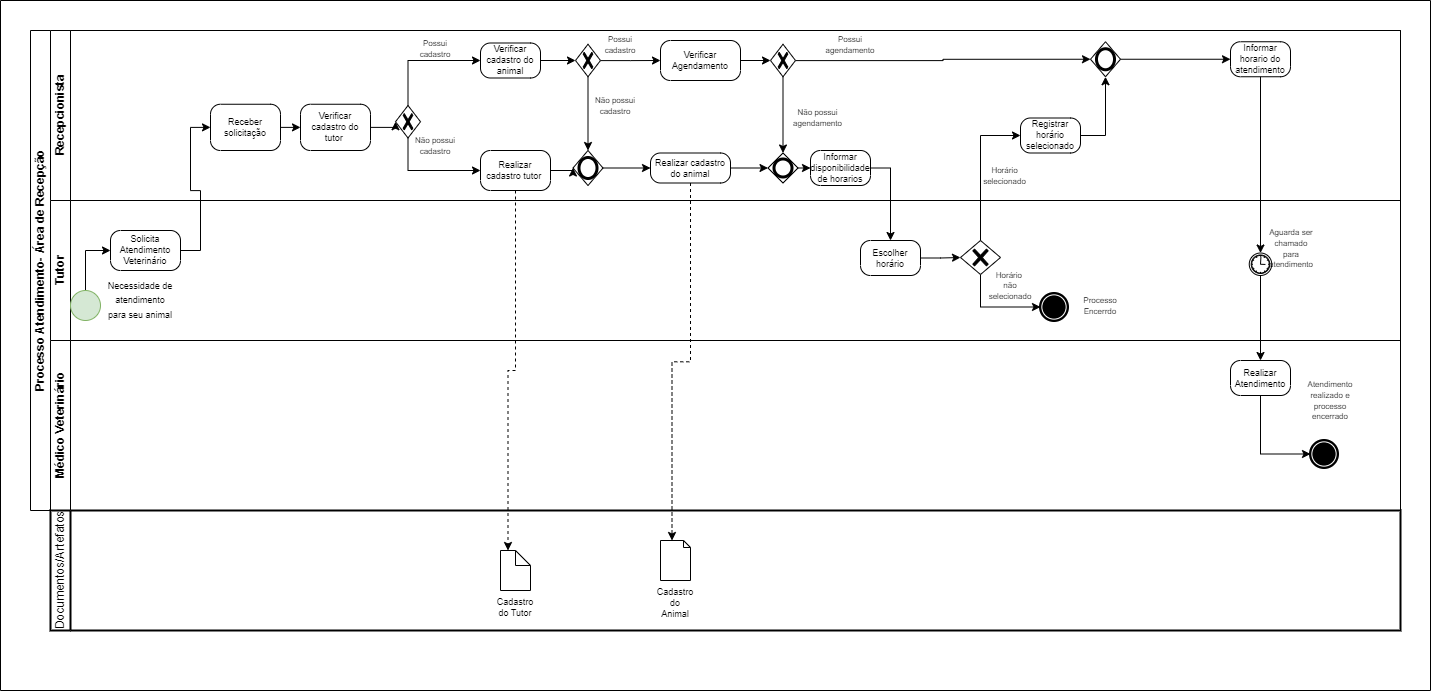
\includegraphics[width=0.9\textwidth]{images/fluxo de atendimento-rec.png}
        \label{fluxo-rec}
    \end{sidewaysfigure}  

    \subsection{ Atendimento Veterinário - Consulta}
    Processo de Consulta adaptado de \citeonline{Rabelo:2012},
    
    
    Processos Antes da Consulta:
	
	\begin{itemize}
	    \item Sala de Atendimento:
            \begin{itemize}
                \item Veterinário abre sistema verifica qual animal será atendido.
                \item Acessa cadastro do animal que será atendido, com seus dados gerais e dados do tutor.
            \end{itemize}
	\end{itemize}
		
		
    \begin{itemize}
        \item Transição:
            \begin{itemize}
                \item Auxiliar encaminha animal e tutor pra sala de atendimento.
                \item Veterinário cria novo prontuário de atendimento (Caso seja retorno, clicar na opção retorno e \emph{linkar} com prontuário de atendimento inicial (para comparar evolução de quadro)).
            \end{itemize}
    \end{itemize}

    \begin{itemize}
        \item Início do Atendimento / Consulta 

        \begin{itemize}
            \item Auxiliar pesa animal e informa veterinário
            \item Veterinario insere peso no campo Peso do Prontuário.
            \item Veterinário preenche campo Queixa Principal.
            \item Veterinário preenche campo Anamnese 
            \item Veterinário realiza exame físico (Estado de consciência, Temperatura, FC, FR, Grau de Desidratação, TPC, Cor de mucosa, Sensibilidade/ Dor)
            \item Veterinário passa dados coletados para o Prontuário.
            \item Veterinário preenche campo Suspeita Diagnóstica.
            \item Veterinário preenche campo Exames, caso necessário, e marca retorno (Abre Agendamento?).
            \item Veterinário encaminha para medicação -> caso necessário e anota medicação utilizada.
            \item Veterinário preenche campo de Medicação utilizada e dose -> alerta para medicamentos controlados.
            \item Veterinário prescreve medicação para tutor, caso necessário, e preenche campo Prescrições.
                        
        \end{itemize}
        \item Veterinário Finaliza Processo.
    \end{itemize}

	
  



     
    \section{Análise de Requisitos}
    
        Na etapa de análise de requisitos, a equipe passa a elaborar em maior nível de detalhamento as regras e características que a aplicação deve suportar, compreendendo de maneira mais assertiva as principais necessidades do cliente e definindo as prioridades do projeto.
        
        Esse é um processo evolutivo incremental em que a equipe deve se reunir com o \emph{Product} \emph{Owner} em frequência definida a fim de refinar os requisitos levantados para o andamento das histórias registradas como itens do \emph{product} \emph{backlog}. 
        
        Conforme as histórias são desenvolvidas, os membros da equipe criarão tarefas de acordo com o entendimento do refinamento discutido.
        
        Partindo das regras de negócio, são apresentados os requisitos funcionais, não funcionais e, por fim, as histórias de usuário.

        \subsection{Regras de Negócio}
        
            As regras de negócio são as premissas necessárias para a modelagem do projeto e através delas serão definidas as regras básicas as quais o sistema deve concernir.
            
            Tem por objetivo explicitar as restrições a serem adotadas pelo sistema a fim de garantir assertividade ao escopo definido para completude das ferramentas e histórias em desenvolvimento, bem como as interdependências entre as ferramentas e historias relacionadas.
            
            O Quadro \ref{tab:regra} dispõe das informações referente às regras de negócios do CertVet:

            \begin{center}
                \begin{quadro}[H]
                \caption{Regras de Negócio}
                \begin{tabulary}{1.0\textwidth}{|C|p{23em}|C|}
                \hline
                
                 Código & Descrição & Requisito Relacionado\\
                \hline
                RN01 & Somente usuário autenticado pode ter acesso ao sistema & RF01\\
                \hline
                RN02 & O usuário deve se autenticar informando seu e-mail e senha de cadastro. & RF02\\
                \hline
                RN03 & O usuário terá acesso às funcionalidades de acordo com o seu tipo de conta. & \\
                \hline
                RN04 & Apenas profissionais com número de CRMV válido devem ter acesso às funcionalidades clínicas. & \\
                \hline
                RN05 & Os prontuários digitais devem seguir o padrão dos modelos oficiais \citeonline {doc_obrig}. & RF10\\
                \hline
                RN06 & Somente usuários com autorização podem realizar edições nos prontuários. & RF11\\
                \hline
                RN07 & Na gestão de medicamentos, a retirada deve ser feita apenas por profissionais veterinários autorizados. & RF14 e RF15\\
                \hline
                RN08 & O controle de vacinação deve ser visível por todas as partes envolvidas, profissionais e tutores. & RF16, RF17 e RF18\\
                \hline
                \end{tabulary}   
                \label{tab:regra}
                \centering
                \footnotesize {Fonte: Elaborado pelos autores.}
                \end{quadro}
            \end{center}

        \subsection{Requisitos Funcionais}
        
            Nos Quadros \ref{tab:req_func} e \ref{tab:req_func2} são apresentados os requisitos funcionais, detalhando as necessidades e especificações das ações que o sistema deve executar, ignorando as limitações físicas, focando apenas no comportamento de entrada e saída do sistema.
            
            \begin{center}
                \begin{quadro}[H]
                \caption{Requisitos Funcionais}
                \begin{tabulary}{1.0\textwidth}{|p{5em}|p{8em}|p{18em}|}
                \hline
                Código & Requisito & Descrição\\
                \hline
                RF01 & Criar conta & O usuário deve criar uma conta de acordo com a sua ocupação (Veterinário | Auxiliar) e seus dados.\\
                \hline
                RF02 & Autenticar usuário & O sistema deve permitir que o usuário entre em sua conta já criada no sistema.\\
                \hline
                RF03 & Alterar senha & O sistema deve permitir que o usuário altere a sua senha.\\
                \hline
                RF04 & Redefinição de senha & O sistema deve permitir que o usuário solicite a redefinição de sua senha.\\
                \hline
                RF05 & Agendar consultas & O sistema deve permitir que o usuário autenticado agende consulta, informando data, horário, paciente e profissional responsável após verificar que este não possui nenhuma consulta já marcada no horário informado.\\
                \hline
                RF06 & Cancelar consulta & O sistema deve permitir que o usuário autenticado cancele uma consulta já agendada.\\
                \hline
                RF07 & Cadastrar tutor & O sistema deve permitir que o usuário autenticado cadastre os dados do tutor do paciente, permitindo também sua consulta e edição.\\
                \hline
                RF08 & Cadastrar animal & O sistema deve permitir que o usuário autenticado cadastre os dados do animal, permitindo também sua consulta e edição.\\
                \hline
                RF09 & Visualizar histórico de consultas & O sistema deve permitir que todos os usuários consultem o histórico de consultas já realizadas, informando dados do paciente.\\
                \hline
                RF10 & Criar prontuário & O sistema deve permitir que o veterinário crie o prontuário digital de atendimento do paciente.\\
                \hline
                RF11 & Editar prontuário de atendimento & O sistema deve permitir que o veterinário edite informações específicas do prontuário digital de atendimento do paciente.\\
                \hline
                RF12 & Verificar histórico de alterações no prontuário & O sistema deve permitir que todos os usuários consultem o histórico de alterações feitas no prontuário digital de atendimento do paciente.\\
                \hline
                \end{tabulary}
                \label{tab:req_func}
                \centering
                
                \footnotesize {Fonte: Elaborado pelos autores.}
                \end{quadro}
            \end{center}
            
            
            \begin{center}
                \begin{quadro}[h]
                \caption{Requisitos Funcionais - continuação}
                \begin{tabulary}{1.0\textwidth}{|p{5em}|p{8em}|p{18em}|}
                \hline
                Código & Requisito & Descrição\\
                \hline
                RF13 & Visualizar aspectos hereditários & O sistema deve permitir que seja visível, ao usuário autenticado, o histórico de aspectos hereditários do animal, quando este possuí-lo.\\
                \hline
                RF14 & Registar consumo de medicamento & O sistema deve permitir que o veterinário autorizado registre o uso de medicamento no prontuário digital do paciente, quando usado no atendimento.\\
                \hline
                RF15 & Visualizar histórico de medicamento & O sistema deve permitir que o usuário consulte o histórico do uso de medicamento, quando usado no atendimento.\\
                \hline
                RF16 & Aplicar vacina & O sistema deve permitir que o veterinário preencha o prontuário específico para vacinação do paciente e que os dados sejam inseridos na ficha do animal.\\
                \hline
                RF17 & Visualizar carteirinha de vacinação & O sistema deve permitir a visualização das vacinas já aplicadas no paciente.\\
                \hline
                RF18 & Visualizar vacinas agendadas & O sistema deve permitir visualização das vacinas agendadas para aplicação no paciente.\\
                \hline
                \end{tabulary}
                \label{tab:req_func2}
                \centering
                
                \footnotesize {Fonte: Elaborado pelos autores.}
                \end{quadro}
            \end{center}

        \subsection{Requisitos não Funcionais}

            Os requisitos não funcionais tratam-se de restrições mais técnicas do projeto, são as necessidades que não são atendidas necessariamente através de funcionalidades, objetivando garantir níveis satisfatórios  de desempenho, disponibilidade, escalabilidade, dentre outras garantias que permitam a máxima usabilidade do sistema. Os requisitos não funcionais que compreendem à CertVet são elencados no Quadro \ref{tab:req_nfunc}.

            \begin{center}
                \begin{quadro}[h]
                  \caption{Requisitos Não Funcionais}
                \begin{tabulary}{1.0\textwidth}{|C|p{25em}|p{7em}|}
                \hline
                Código & Requisito & Categoria\\
                \hline
                RNF01 & O sistema deve estar disponível para o usuário de acordo com o funcionamento da clínica, podendo ser utilizado 24 horas por dia, 7 dias por semana, com tolerância de 0,1\% de falhas. & Disponibilidade\\
                \hline
                RNF02 & O sistema deve ser implementado de forma que seja apto para crescimento, visando suportar a entrada de novos usuários e novas funcionalidades, sem comprometer seu desempenho e segurança. & Escalabilidade, Portabilidade\\
                \hline
                RNF03 & O sistema deve atender ao Artigo 8 da Lei nº 5.517, prevendo a fiscalização do exercício profissional pelos Conselhos Federal e Regionais de Medicina Veterinária. & Legalidade\\
                \hline
                RNF04 & As documentações criadas e utilizadas no sistema devem seguir a padronização de elaboração, fornecimento e guarda, conforme Resolução 1071/2014, também do Conselho Federal de Medicina Veterinária. & Legalidade\\
                \hline
                RNF05 & O sistema deve atender às especificações da Lei Geral de Proteção de Dados (Lei 13.709/18), garantindo a segurança dos dados dos usuários, animais e tutores. & Legalidade\\
                \hline
                RNF06 & O sistema deve ter sua interface organizada de forma que o usuário consiga utilizar suas funcionalidades sem dificuldades de operá-las. & Usabilidade\\
                \hline
                RNF07 & O sistema deve compreender tecnologia de internacionalização, a fim de promover sua tradução para diferentes idiomas. & Usabilidade\\
                \hline
                RNF08 & O sistema deve contar com um protocolo criptografado e seguro de transferência de dados em sua implementação. & Segurança\\
                \hline
                RNF09 & O sistema deve apresentar um layout que seja adaptável para as dimensões de tela de diferentes dispositivos, garantindo responsividade. & Usabilidade\\
                \hline
                \end{tabulary}
                \label{tab:req_nfunc}
                \centering
                
               \footnotesize Fonte: Elaborado pelos autores.
                \end{quadro}
            \end{center}

\subsection{Histórias de Usuários}

    
    \begin{center}
        \begin{quadro}[H]
        \caption{Histórias de Usuário}
        \begin{tabulary}{1.0\textwidth}{|p{5em}|p{8em}|p{18em}|}
        \hline
        Código & História & Descrição\\
        \hline
        HU-01 & Função gerar documento com assinatura digital/certificação & Eu como usuário autorizado, quero gerar um documento oficial com assinatura digital, que me permita rastrear todas suas versões anteriores, para que sejam rastreáveis e passíveis de identificação.\\
        \hline
        HU-02 & Função preencher prontuário & Eu como usuário autorizado, quero preencher um prontuário para um animal em atendimento, para que seus dados sejam salvos.\\
        \hline
        HU-03 & Função salvar prontuário & Eu como usuário autorizado, quero salvar o prontuário digital, para que seja possível sua leitura em momento posterior.\\
        \hline
        HU-04 & Função uso de medicamentos controlados & Eu como usuário autorizado, quero anotar os medicamentos controlados utilizados no atendimento, para que seja possível seu controle com os dados do estoque.\\
        \hline
        HU-05 & Função inserir medicamentos no estoque & Eu, como usuário autorizado, quero inserir no sistema a quantidade total de produtos no estoque, para que seja possível o controle de quantidade usada por atendimento, perdida e que ainda está disponível.\\
        \hline
        HU-06 & Função visualizar prontuários & Eu, como usuário autorizado, quero acessar os prontuários de determinado animal, para que seja possível acompanhar seu histórico ou quadro clínico.\\
        \hline
        HU-07 & Função salvar dados hereditários &  Eu, como usuário autorizado, quero inserir dados sobre pais e descendentes (quando existentes), na ficha médica do animal, para que tais dados estejam disponíveis para consulta quando necessário.\\
        \hline
        HU-08 &  Função recuperar aspectos hereditários &  Eu, como usuário autorizado, quero consultar aspectos hereditários do animal (quando disponível), para obter informações úteis ao tratamento do mesmo.\\
        \hline
        HU-09 & Função inserir dados na agenda & Eu, como funcionário, quero inserir dados de um atendimento na agenda, para que os atendimentos futuros sejam planejados.\\
        \hline
        HU-10 & Função cadastrar cliente & Eu, como funcionário, quero cadastrar um cliente no sistema, para que seus dados estejam disponíveis para uso dentro da clínica\\
        \hline
        \end{tabulary}
        
        \label{tab:hist_usuario}
        \centering
        {\footnotesize Fonte: Elaborado pelos autores.}
        \end{quadro}
    \end{center}

    \section{Modelagem}
    
        \subsection{Modelo Entidade Relacionamento}
        
            \begin{figure}[H]
            \centering
                \caption{Modelo Entidade Relacionamento}
                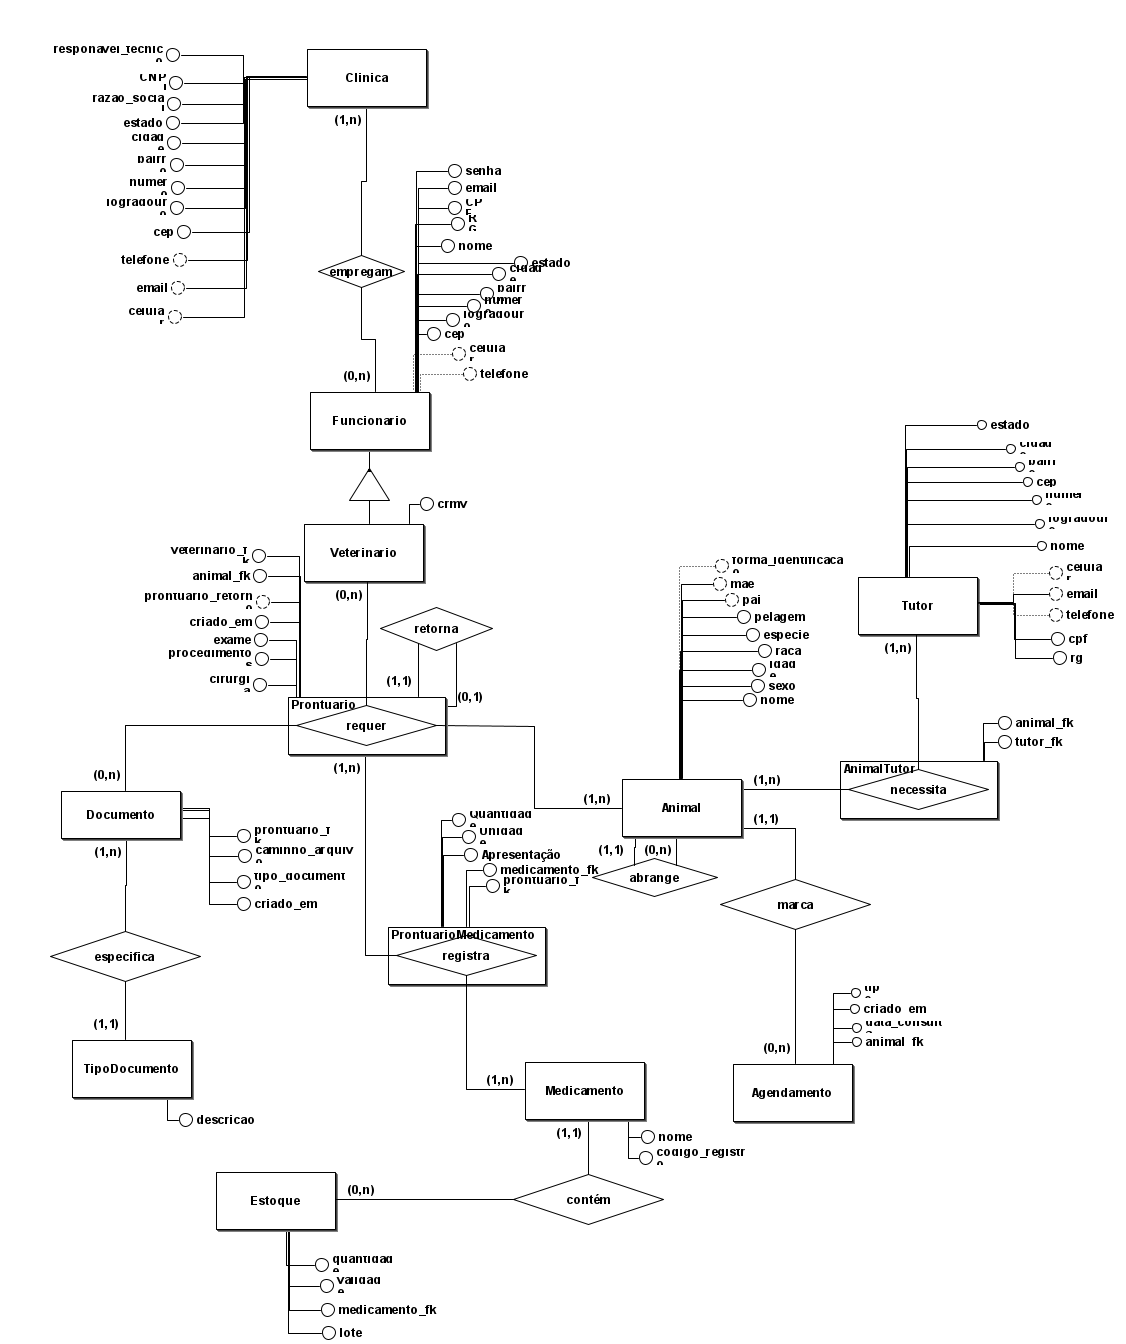
\includegraphics[ width=\linewidth]{images/ProjetoPI1.2 .png}
                
                \label{fig:MER}
                \centering
                {\footnotesize Fonte: Elaborado pelos autores.}
            \end{figure}
    
            \begin{center}
                \begin{quadro}[H]
                \centering
                \caption{Entidades do \nameref{fig:MER} }
                \begin{tabulary}{1.0\textwidth}{|p{10em}|p{26em}|}
                \hline
                Entidade & Descrição\\
                \hline
                Prontuário & Entidade em que é armazenado os dados do atendimento de um animal. \\
                \hline
                Veterinário & Entidade em que é armazenado os dados do profissional veterinário.\\
                \hline
                Animal & Entidade em que é armazenado os dados do animal.\\
                \hline
                Medicamento & Entidade em que é armazenado os dados do medicamento.\\
                \hline
                ProntuárioMedicamento & Entidade em que é associado o medicamente com a quantidade utilizada no atendimento.\\
                \hline
                Estoque & Entidade que armazena a quantidade disponível do medicamento.\\
                \hline
                Clínica & Entidade que armazena dados referentes ao estabelecimento veterinário.\\
                \hline
                Tutor & Entidade que armazena dados do tutor/proprietário do animal atendido.\\
                \hline
                AnimalTutor & Entidade que associa um animal com seu tutor.\\
                \hline
                Agendamento & Entidade que registra um animal com horario de atendimento, clínica e tipo de atendimento.\\
                \hline
                Funcionário & Entidade que armazena os dados dos funcionários do estabelecimento.\\
                \hline
                Documento & Entidade que armazena dados comuns referentes a documentos obrigatórios gerados pelo veterinário.\\
                \hline
                TipoDocumento & Entidade que armazena dados específicos de um documento obrigatório.\\
                \hline
                \end{tabulary}
                \label{tab: entidades} \\
                \centering
                {\footnotesize Fonte: Elaborado pelos autores.}
                \end{quadro}
            \end{center}

            \begin{center}
              \begin{quadro}[H]
            
                \caption{Dicionário de Dados - Prontuário}
                \begin{tabulary}{1.0\textwidth}{|p{9em}|c|c|c|p{19em}|}
                \hline
                Atributos & Chave & NN & Tipo & Descrição\\
                \hline
                Veterinário & FK & x & bigint & Identifica o veterinário responsável \\
                \hline
                Animal & FK & x & bigint & Identifica o animal atendido \\
                \hline
                Prontuário_retorno & x & x & boolean & Identifica se o prontuário é de um retorno\\
                \hline
                Criado Em & x & x & timestamp & registro de quando o prontuário foi feito \\
                \hline
                Exame & x & x & varchar & Campo para especificar Exames solicitados\\
                \hline
                Procedimento & x & x & varchar & Campo para especificar procedimentos realizados \\
                \hline
                Cirurgia & x & x & varchar & Campo para especificar quando há necessidade de cirurgia\\
                \hline
                Prontuário & PK & x & bigint & Identificação do prontuário \\
                \hline
                \end{tabulary}
                \label{qd: md-prontuario}
                \centering
                \footnotesize Fonte: Elaborado pelos autores.
                \end{quadro}
                \end{center}
    
            \begin{center}
              \begin{quadro}[H]
              \centering
                  \caption{Dicionário de Dados - Veterinário}
                  \begin{tabulary}{1.0\textwidth}{|p{9em}|c|c|c|p{19em}|}
                \hline
                Atributos & Chave & NN & Tipo & Descrição\\
                \hline
                ID & PK & x & BIGINT & Atributo de Identificação do médico veterinário \\
                \hline
                CRMV & - & x & varchar & Atributo que guarda o registro do médico veterinário\\
                \hline
                \end{tabulary}
                 
                  \label{qd: md-veterinario}
                  \centering
        {\footnotesize Fonte: Elaborado pelos autores.}
              \end{quadro}
            \end{center}
    
            \begin{center}
              \begin{quadro}[H]
              \centering
                  \caption{Dicionário de Dados - Animal}
                  \begin{tabulary}{1.0\textwidth}{|p{9em}|c|c|c|p{19em}|}
                \hline
                Atributos & Chave & NN & Tipo & Descrição\\
                \hline
                ID & PK & x & BIGINT & Identifica a chave do \\
                \hline
                Nome & - & x & varchar & Atributo que guarda o nome do animal\\
                \hline
                Espécie & - & x & varchar & Atributo que recebe a especie do animal\\
                \hline
                Raça & - & x & varchar & Atributo que recebe a raça do animal \\
                \hline
                Sexo & - & x & varchar & Atributo que recebe o sexo do animal\\
                \hline
                Idade & - & x & BIGINT & Atributo que recebe a idade do animal\\
                \hline
                Pelagem & - & - & varchar & Atributo que recebe o tipo de pelagem do animal \\
                \hline
                Forma\_identificação & - & - & varchar & Atributo que recebe a identificação do animal\\
                \hline
                Mãe & FK & - & BIGINT & Atributo que identifica a mãe do animal \\
                \hline
                Pai & FK & - & BIGINT & Atributo que identifica o pai do animal \\
                \hline
                \end{tabulary}
                 
                  \label{qd: md-animal}
                  \centering
        {\footnotesize Fonte: Elaborado pelos autores.}
              \end{quadro}
            \end{center}
    
    \begin{center}
      \begin{quadro}[H]
      \centering
          \caption{Dicionário de Dados - Medicamento}
          \begin{tabulary}{1.0\textwidth}{|p{9em}|c|c|c|p{19em}|}
        \hline
        Atributos & Chave & NN & Tipo & Descrição\\
        \hline
        Id & PK & x & BIGINT & Atributo que identifica o medicamento\\
        \hline
        Código\_Registro & - & x & BIGINT & Atributo que identifica o código do medicamento\\
        \hline
        Nome & - & x & varchar & Atributo que identifica o nome do medicamento\\
        \hline
        \end{tabulary}
         
          \label{qd: md-medicamento}
          \centering
        {\footnotesize Fonte: Elaborado pelos autores.}
      \end{quadro}
    \end{center}
    
    \begin{center}
      \begin{quadro}[H]
      \centering
          \caption{Dicionário de Dados - ProntuárioMedicamento}
          \begin{tabulary}{1.0\textwidth}{|p{9em}|c|c|c|p{19em}|}
        \hline
        Atributos & Chave & NN & Tipo & Descrição\\
        \hline
        Prontuário & FK & x & BIGINT & Identificação do Prontuário \\
        \hline
        Medicação & FK & x & BIGINT & Atributo que identifica o medicamento utilizado \\
        \hline
        Apresentação & - & x & varchar & Atributo que recebe o tipo de apresentação do medicamento\\
        \hline
        Quantidade & - & x & BIGINT & Atributo que recebe a quantidade do medicamento utilizada\\
        \hline
        Unidade & - & x & varchar & Atributo que recebe a unidade do medicamento \\
        \hline
        \end{tabulary}
         
          \label{qd: md-prontuariomedicamento}
          \centering
        {\footnotesize Fonte: Elaborado pelos autores.}
      \end{quadro}
    \end{center}
    
    \begin{center}
      \begin{quadro}[H]
      \centering
          \caption{Dicionário de Dados - Estoque}
          \begin{tabulary}{1.0\textwidth}{|p{9em}|c|c|c|p{19em}|}
        \hline
        Atributos & Chave & NN & Tipo & Descrição\\
        \hline
        Medicamento & FK & x & BIGINT & Atributo que identifica o medicamento\\
        \hline
        Lote & - & x & BIGINT & Atributo que recebe o lote do medicamento\\
        \hline
        Validade & - & x & timestamp & Atributo que recebe a data de validade do medicamento \\
        \hline
        Quantidade & - & x & BIGINT & Atributo que recebe a quantidade de medicamento total do estoque \\
        \hline
        \end{tabulary}
         
          \label{qd: md-estoque}
          \centering
        {\footnotesize Fonte: Elaborado pelos autores.}
      \end{quadro}
    \end{center}
    
    \begin{center}
      \begin{quadro}[H]
      \centering
          \caption{Dicionário de Dados - Clínica}
          \begin{tabulary}{1.0\textwidth}{|p{9em}|c|c|c|p{19em}|}
        \hline
        Atributos & Chave & NN & Tipo & Descrição\\
        \hline
        ID & PK & x & BIGINT & Atributo que identifica a clínica \\
        \hline
        Razao Social & - & x & varchar & Atributo que guarda o nome da clínica\\
        \hline
        CNPJ & - & x & BIGINT & Atributo que guarda o CNPJ da clínica \\
        \hline
        Responsável Técnico & FK & x & varchar & Atributo que recebe o nome do funcionario veterinário cadastrado como RT\\
        \hline
        Telefone & - & x & varchar & Atributo que recebe o telefone da clínica\\
        \hline
        Email & - & x & varchar & Atributo que recebe o email da clínica\\
        \hline
        Celular & - & x & varchar & Atributo que recebe o celular da clínica \\
        \hline
        Estado & - & x & varchar & Atributo que recebe o estado da clínica\\
        \hline
        Cidade & - & x & varchar & Atributo que recebe a cidade da clínica \\
        \hline
        Bairro & - & x & varchar & Atributo que recebe o bairro da clínica \\
        \hline
        Logradouro & - & x & varchar & Atributo que recebe o nome da rua da clínica\\
        \hline
        Número & - & x & varchar & Atributo que recebe o número da clínica \\
        \hline
        CEP & - & x & varchar &  Atributo que recebe o CEP da clinica\\
        \hline
        \end{tabulary}
         
          \label{qd: md-clinica}
          \centering
        {\footnotesize Fonte: Elaborado pelos autores.}
      \end{quadro}
    \end{center}
    
    \begin{center}
      \begin{quadro}[H]
      \centering
          \caption{Dicionário de Dados - Tutor}
          \begin{tabulary}{1.0\textwidth}{|p{9em}|c|c|c|p{19em}|}
        \hline
        Atributos & Chave & NN & Tipo & Descrição\\
        \hline
        ID & PK & x & BIGINT & Atributo que identifica o tutor \\
        \hline
        Nome & - & x & varchar & Atributo que guarda o nome do tutor\\
        \hline
        Rg & - & x & varchar & Atributo que recebe o rg do tutor \\
        \hline
        CPF & - & x & varchar & Atributo que recebe o CPF do tutor\\
        \hline
        Email & - & x & varchar & Atributo que recebe o email do tutor\\
        \hline
        Telefone & - & x & varchar & Atributo que recebe o telefone do tutor\\
        \hline
        Celular & - & x & varchar & Atributo que recebe o celular do tutor\\
        \hline
        Estado & - & x & varchar & Atributo que recebe o estado do tutor\\
        \hline
        Cidade & - & x & varchar & Atributo que recebe a cidade do tutor\\
        \hline
        Bairro & - & x & varchar & Atributo que recebe o bairro do tutor\\
        \hline
        Logradouro & - & x & varchar & Atributo que recebe o nome da rua do tutor\\
        \hline
        Numero & - & x & varchar & Atributo que recebe o numero de residencia do tutor\\
        \hline
        CEP & - & x & varchar & Atributo que recebe o CEP do tutor\\
        \hline
        \end{tabulary}
         
          \label{qd: md-tutor}
          \centering
        {\footnotesize Fonte: Elaborado pelos autores.}
      \end{quadro}
    \end{center}
    
    \begin{center}
      \begin{quadro}[H]
      \centering
          \caption{Dicionário de Dados - AnimalTutor}
          \begin{tabulary}{1.0\textwidth}{|p{9em}|c|c|c|p{19em}|}
        \hline
        Atributos & Chave & NN & Tipo & Descrição\\
        \hline
        Tutor & FK & x & BIGINT & Atributo que identifica o tutor. \\
        \hline
        Animal & FK & x & BIGINT & Atributo que identifica o animal.\\
        \hline
        \end{tabulary}
         
          \label{qd: md-animaltutor}
          \centering
        {\footnotesize Fonte: Elaborado pelos autores.}
      \end{quadro}
    \end{center}
    
    \begin{center}
      \begin{quadro}[H]
      \centering
          \caption{Dicionário de Dados - Agendamento}
          \begin{tabulary}{1.0\textwidth}{|p{9em}|c|c|c|p{19em}|}
        \hline
        Atributos & Chave & NN & Tipo & Descrição\\
        \hline
        %ID & PK & x & BIGINT & Atributo que identifica o agendamento \\
        |%\hline
        Animal & FK & x & BIGINT & Atributo que identifica o animal que passará por atendimento \\
        \hline
        Tipo & - & x & varchar & Atributo que recebe o tipo de atendimento será realizado \\
        \hline
        Criado\_Em & - & x & timestamp & Atributo que guarda a data quando foi realizado o agendamento\\
        \hline
        Data\_Consulta & - & x & timestamp & Atributo que guarda a data a ser realizado o atendimento \\
        \hline
        \end{tabulary}
         
          \label{qd: md-agendamento}
          \centering
        {\footnotesize Fonte: Elaborado pelos autores.}
      \end{quadro}
    \end{center}
    
    \begin{center}
      \begin{quadro}[H]
      \centering
          \caption{Dicionário de Dados - Funcionário}
          \begin{tabulary}{1.0\textwidth}{|p{9em}|c|c|c|p{19em}|}
        \hline
        Atributos & Chave & NN & Tipo & Descrição\\
        \hline
        ID & PK & x & BIGINT & Atributo que identifica o funcionário no sistema \\
        \hline
        Nome & - & x & varchar & Atributo que recebe o nome do funcionário \\
        \hline
        RG & - & x & varchar & Atributo que recebe o RG do funcionário\\
        \hline
        CPF & - & x & varchar & Atributo que recebe o CPF do funcionário\\
        \hline
        Senha & - & x & varchar & Atributo da senha de acesso do funcionário ao sistema\\
        \hline
        Telefone & - & - & varchar & Atributo que recebe o contato telefônico do funcionário\\
        \hline
        Celular & - & x & varchar & Atributo que recebe o contato móvel do funcionário \\
        \hline
        Email & - & x & varchar & Atributo que recebe o endereço eletrônico do funcionário\\
        \hline
        Estado & - & - & varchar & Atributo que recebe o estado da residência do funcionário\\
        \hline
        Cidade & - & - & varchar & Atributo que recebe a cidade da residência do funcionário\\
        \hline
        Bairro & - & - & varchar & Atributo que recebe o bairro da residência do funcionário\\
        \hline
        Logradouro & - & - & varchar & Atributo que recebe a rua da residência do funcinário \\
        \hline
        Número & - & - & int & Atributo que recebe a numeração da residencia do funcionário\\
        \hline
        CEP & - & - & varchar & Atributo que recebe o CEP do funcionário\\
        \hline
        \end{tabulary}
         
          \label{qd: md-funcionario}
          \centering
        {\footnotesize Fonte: Elaborado pelos autores.}
      \end{quadro}
    \end{center}
    
    \begin{center}
      \begin{quadro}[H]
      \centering
          \caption{Dicionário de Dados - Documento}
          \begin{tabulary}{1.0\textwidth}{|p{9em}|c|c|c|p{19em}|}
        \hline
        Atributos & Chave & NN & Tipo & Descrição\\
        \hline
        Prontuário & FK & x & BIGINT & Identificação do Prontuário \\
        \hline
        Tipo\_Documento & FK & x & BIGINT & Atributo que identifica tipo  de autorização \\
        \hline
        Caminho\_Arquivo & - & x & varchar & identifica a url do arquivo na AWS\\
        \hline
        Criado\_Em & - & x & timestamp & Atributo que identifica a data de criação do documento\\
        \hline
        \end{tabulary}
         
          \label{qd: md-documento}
          \centering
        {\footnotesize Fonte: Elaborado pelos autores.}
      \end{quadro}
    \end{center}
    
    \begin{center}
      \begin{quadro}[H]
      \centering
          \caption{Dicionário de Dados - TipoDocumento}
          \begin{tabulary}{1.0\textwidth}{|p{9em}|c|c|c|p{19em}|}
        \hline
        Atributos & Chave & NN & Tipo & Descrição\\
        \hline
        ID & PK & x & BIGINT & Atributo que identifica o documento\\
        \hline
        Descrição & - & - & varchar & Descreve qual tipo de documento\\
        \hline
        \end{tabulary}
         
          \label{qd: md-tipodocumento}
          \centering
        {\footnotesize Fonte: Elaborado pelos autores.}
      \end{quadro}
    \end{center}
    
 
    
    
        \subsection{Diagrama Entidade-Relacionamento}
        
            \begin{figure}[H]
                \centering
                \caption{Diagrama Entidade-Relacionamento}
                \includegraphics[width=0.7\textwidth]{images/Modelo Lógico.png}
                
                \label{fig:DER}
                \centering
        {\footnotesize Fonte: Elaborado pelos autores.}
            \end{figure}

    \section{Gestão e organização da equipe}

        \subsection{Organização da Equipe}
            
            O guia do \emph{scrum} declara explícitamente que o time deve ser pequeno suficiente para que seja ágil e grande o suficiente para que possa desempenhar trabalho relevante, recomendando o envolvimento de não mais que 10 integrantes \citeonline{scrum2}.
            
            Orientados pela recomendação de formação de papéis da equipe ágil \emph{Scrum}, foram definidos 3 papéis para ser desempenhado pelos membros da equipe: \emph{Product Owner} (PO -  Dono do Produto), \emph{scrum Master} (SCM - Mestre do Scrum) e \emph{Developers}, que foram denominados \emph{Team Members} (TM - Membros da equipe). Esses papéis têm o objetivo de apontar facilitadores e atribuir responsabilidades em pontos específicos do projeto, não havendo um responsável isolado ou encarregado do bom desenvolvimento das atividades.\citeonline{scrum2} \citeonline{agile2}
            
            O PO é responsável por definir clara e objetivamente como as funcionalidades da aplicação devem se comportar, compreender e priorizar a necessidade de negócio que melhor atende a necessidade do usuário (\emph{stakeholders}) e que o \emph{backlog }seja visível e disponível para todos os membros do time.\citeonline{agile2} O papel será desempenhado pela Irina Chang.
            
            O SCM tem a responsabilidade que o time consiga desenvolver autonomia, destravando entendimentos e facilitando a identificação de dinâmicas que resultem em melhor entregabilidade das atividades.\citeonline{agile2} O papel será desempenhado por Henrique.
            
            \emph{Team Member} é a forma como foi decidido denominar o papel dos desenvolvedores. Estes serão os responsáveis pela implementação de código, padronização de commits, integrações, modelagem de banco de dados, além de verificar se as alterações propostas pelo PO são tecnicamente viáveis de serem implementadas, definindo os processos necessários para a implementação. Por consequência, são os maiores responsáveis pelo desenvolvimento da documentação do código e garantia da manutenibilidade. Independentemente do envolvimento anterior, são responsáveis por auxiliar em  manutenções futuras e realizar a entrega (\emph{deploy}) da aplicação em produção.\citeonline{scrum2} Os team members são: Caique Daniel, Luis Renato, Marcos Querino, Murilo Pires e Welen Mota.
            
            Entretanto, diferentemente do papel do Scrum, o time conta com indivíduos com conhecimentos e habilidades diversas e tempo limitado para o desenvolvimento do projeto. Dessa forma, os papeis servirão como referência, mas não limitam os indivíduos às atividades definidas pelos papéis do Scrum.
            
            Todos os membros escreveram diferentes partes da documentação, textos que eram revisados posteriormente pelos outros integrantes. O controle de versionamento também foi tarefa de todos os integrantes. A geração de métricas e envios para versionamento na SVN, apesar de ser de conhecimento de todos, mas devido a diferentes problemas técnicos enfrentados por alguns integrantes, não pode ser efetuada por todos os membros. A correção dessas falhas estão planejadas para o período de recesso do ano letivo, para não atrapalhar o andamento do resto do projeto. O desenvolvimento da parte técnica do projeto, relativo a codificação (\emph{front-end} e \emph{back-end}) e infraestrutura levou em conta o conhecimento prévio de cada integrante, sua familiaridade com as tecnologias e capacidade de desenvolver a aplicação em tempo hábil. Com isso, alguns membros com menor grau de familiaridade com a tecnologia, participavam dos \emph{pair-programming} como observadores, ajudando a identificar possíveis erros no código, o que contribuiu para maior aprendizado dos mesmos e aprofundar o conhecimento de todos em todas as partes do projeto.
            
             O Quadro \ref{tab:membros} foi elaborado para facilitar a identificação da ênfase de atuação de cada indivíduo sobre as atividades desempenhadas.

        \begin{center}
            \begin{quadro}[H]
            \centering
            \caption{Membros}
            \resizebox{16cm}{!}{%
                \begin{tabular}{|p {15}|rrrrrrrr|}
                \hline
                \multicolumn{1}{|c|}{Membro}      & \multicolumn{1}{c|}{Irina}   & \multicolumn{1}{r|}{Henrique} & \multicolumn{1}{r|}{Caique}       & \multicolumn{1}{r|}{Luís} &
                \multicolumn{1}{r|}{\begin{tabular}[c]{@{}c@{}}Marcos \end{tabular}}  &
                \multicolumn{1}{r|}{Murilo} & \multicolumn{1}{r|}{Welen}\\ \hline
               
            \multicolumn{1}{|l|}{\begin{tabular}[c]{@{}c@{}}Documentação \end{tabular}} &
            \multicolumn{1}{c|}{x}  & \multicolumn{1}{c|}{x}  & \multicolumn{1}{c|}{x}  & \multicolumn{1}{c|}{x}  & \multicolumn{1}{c|}{x}  & \multicolumn{1}{c|}{x}  & \multicolumn{1}{c|}{x}            \\ \hline
                    
        \multicolumn{1}{|l|}{\begin{tabular}[c]{@{}c@{}}Versionamento \end{tabular}} &
            \multicolumn{1}{c|}{x}  & \multicolumn{1}{c|}{x}  & \multicolumn{1}{c|}{x}  & \multicolumn{1}{c|}{x}  & \multicolumn{1}{c|}{x}  & \multicolumn{1}{c|}{x}  & \multicolumn{1}{c|}{x}            \\ \hline
            \multicolumn{1}{|l|}{\begin{tabular}[c]{@{}c@{}}Métricas\end{tabular}} &
             \multicolumn{1}{c|}{x}  & \multicolumn{1}{c|}{x}  & \multicolumn{1}{c|}{ }  & \multicolumn{1}{c|}{ }  & \multicolumn{1}{c|}{ }  & \multicolumn{1}{c|}{ }  & \multicolumn{1}{c|}{x}            \\ \hline
        \multicolumn{1}{|l|}{\begin{tabular}[c]{@{}c@{}}\emph{Front-end} \end{tabular}}&                 
            \multicolumn{1}{c|}{ }  & \multicolumn{1}{c|}{ }  & \multicolumn{1}{c|}{ x }  & \multicolumn{1}{c|}{x}  & \multicolumn{1}{c|}{x}    & \multicolumn{1}{c|}{ }  & \multicolumn{1}{c|}{ }            \\ \hline
 
        \multicolumn{1}{|l|}{\begin{tabular}[c]{@{}c@{}}\emph{Back-End} \end{tabular}} &
            \multicolumn{1}{c|}{x} & \multicolumn{1}{c|}{x}  & \multicolumn{1}{c|}{} & \multicolumn{1}{c|}{}  & \multicolumn{1}{c|}{} & \multicolumn{1}{c|}{x}  & \multicolumn{1}{c|}{}            \\ \hline
                  
    \multicolumn{1}{|l|}{\begin{tabular}[c]{@{}c@{}}Banco de dados \end{tabular}} &
            \multicolumn{1}{c|}{}  & \multicolumn{1}{c|}{}  & \multicolumn{1}{c|}{x} & \multicolumn{1}{c|}{}  & \multicolumn{1}{c|}{}  & \multicolumn{1}{c|}{}  & \multicolumn{1}{c|}{}            \\ \hline
  
        \multicolumn{1}{|l|}{\begin{tabular}[c]{@{}c@{}}Infraestrutura \end{tabular}} &
            \multicolumn{1}{c|}{ }  & \multicolumn{1}{c|}{x} & \multicolumn{1}{c|}{ } & \multicolumn{1}{c|}{ } & \multicolumn{1}{c|}{ } & \multicolumn{1}{c|}{ }  & \multicolumn{1}{c|}{ }            \\ \hline

    \end{tabular}%
       }
        \label{tab:membros}
        \centering
        
        {\footnotesize Fonte: Elaborado pelos autores.}
        \end{quadro}
    \end{center}
            
            % Fonte: https://scrumguides.org/scrum-guide.html#scrum-team
            % Fonte https://www.atlassian.com/br/agile/scrum/roles
            % Revisão fim %
    
        
    \subsection{Gestão de projeto}
    
        % Revisão inicio %
        %Estou com duvidas com relação a esse primeiro paragrafo
        %A partir da avaliação dos requisitos, considerou-se que não existem funcionalidades com processos claramente definidos até o início do desenvolvimento de cada processo e o tempo hábil para elaborar e documentar extensamente todos os processos para serem implementados não é suficiente para que exista código a ser implementado. Portanto, a abordagem de planejamento de projetos cascata não é adequada para desenvolver a solução.
        
        Considerando a restrição temporal definida pelo cronograma acadêmico e os Requisitos Funcionais e Requisitos Não Funcionais já expostos anteriormente nos Quadros \ref{tab:req_func} e \ref{tab:req_nfunc} respectivamente, a equipe decidiu que adotar alguns elementos da metodologia \emph{Scrum} \citeonline{scrum} e a prática do \emph{pair programming} do \emph{Extreme Programming} (XP) \citeonline{agile} seriam melhor adequados às necessidades do projeto. Enfatizando o emprego dos processos, rituais e cerimônias do \emph{Scrum} e apenas complementando com um elemento do método XP para o dia a dia de desenvolvimento, fomentando maior propensão à colaboração e dinamismo de desenvolvimento entre os membros da equipe, resultando em entregas com ritmo constante e incremental.
        
        %mudar sprint para : \emph{sprint} para transformar em itálico 
        
        Os ciclos para o desenvolvimento do projeto foram projetados com duração semanal, denominadas \emph{sprint}. Este processo é definido no \emph{Scrum} como o período em que ocorrem os desenvolvimentos, sendo um dos conceitos centrais da metodologia. Define o escopo que será trabalhado, movendo os itens que passam do \emph{backlog} para a etapa de refinamento e desenvolvimento pela equipe, analisa e desenvolve os elementos que comporão a solução, podendo negociar novos prazos com o PO conforme a equipe identifica novos aprendizados \citeonline{scrum}. Este processo permite melhor acompanhamento da evolução do desenvolvimento, permitindo manter os \emph{stakeholders} atualizados e com expectativas alinhadas.
        
        Ao final de cada \emph{sprint}, ocorre a cerimônia de \emph{Sprint Review} para discutir o processo de aprendizado do período, quais os resultados obtidos e avaliar a evolução da semana, através de debate sobre dificuldades, soluções e impedimentos encontrados no decorrer da \emph{sprint}. Também é realizado o planejamento da \emph{sprint} da semana seguinte, analisando e priorizando os próximos itens que passarão do \emph{backlog} para serem trabalhados no próximo ciclo de desenvolvimento durante as \emph{sprint plannings}, conforme a recomendações de \citeonline{scrum} para o Scrum.
        
        A prática de \emph{pair programing} é adotada para estimular o desenvolvimento colaborativo no time, tal abordagem permite maior compartilhamento dos conhecimentos de cada indivíduo, de forma mais coesa e analisada por pares durante o desenvolvimento do código ou documento. Tal abordagem reduz possíveis atrasos no desenvolvimento decorrentes de dúvidas ou entraves individuais, tendo como consequência a entrega de código com consistência e validação por pares. A abordagem também aumenta o envolvimento do time em relação a entrega de código com qualidade, derivado do sentimento de responsabilidade coletiva que nasce da autonomia para modificações \citeonline{agile}.

        A abordagem aprofunda o conhecimento específico da equipe sobre determinado assunto e da solução construída e incentiva o compartilhamento e comunicação entre os integrantes envolvidos imediatamente durante o desenvolvimento ou durante a \emph{sprint review}.
        
        Nos Quadros \ref{qd:sprints}, \ref{qd: epic} e \ref{qd: backlog} estão relacionadas as informações de desenvolvimento do projeto referentes às \emph{sprints} semanais, divisão de tarefas \emph{Epics} e o \emph{product backlog} do desenvolvimento do projeto.
        % Revisão fim %
        \begin{center}
      \begin{quadro}[H]
      \centering
          \caption{\emph{Sprints}}
          \begin{tabulary}{1.0\textwidth}{|p{8em}|p{8em}|p{19em}|}
        \hline
        Início & Fim & Descrição\\
        \hline
        09/08/2022/ & 16/08/2022 & Definição de grupo e discussão inicial sobre temas. \\
        \hline
        16/08/2022 & 23/08/2022 & Apresentação das propostas aos professores e escolha do projeto.\\
        \hline
        23/08/2022 & 30/08/2022 & Apresentação inicial dos projetos, aprovação do tema e divisão das atividades.\\
        \hline
        30/08/2022 & 06/09/2022 & Início da modelagem da aplicação.\\
        \hline
        06/09/2022 & 13/09/2022 & Início do desenvolvimento da modelagem de dados.\\
        \hline
        13/09/2022 & 20/09/2022 & Escolha da arquitetura da aplicação.\\
        \hline
        20/09/2022 & 27/09/2022 & Discussão de Regras de negócio, Requisitos e Custo do Projeto. \\
        \hline
        27/09/2022 & 04/10/2022 & Apresentação do Desenho da aplicação e definição dos próximos passos. \\
        \hline
        04/10/2022 & 11/10/2022 & Semana de desenvolvimento e preparação para a apresentação da POC. \\
        \hline
        11/10/2022 & 18/10/2022 & Ajustes finais para a apresentação da POC. \\
        \hline
        18/10/2022 & 25/10/2022 & Hands on de implementações e ajustes de documentação.\\
        \hline
        25/10/2022 & 01/11/2022 & Discussão e desenvolvimento da documentação e evolução do MVP da aplicação. \\
        \hline
        01/11/2022 & 08/11/2022 & Desenvolvimento final da documentação e da aplicação do MVP.\\
        \hline
        \end{tabulary}
         
          \label{qd:sprints}
          \centering
         { \footnotesize Fonte: Elaborado pelos autores.}
      \end{quadro}
    \end{center}
    
    %  Criação do backlog  %
    
 \begin{center}
      \begin{quadro}[H]
      \centering
          \caption{\emph{Epics}}
          \begin{tabulary}{1.0\textwidth}{|p{12em}|p{25em}|}
        \hline
       Epic & Descrições  \\
        \hline
        Ajustes Documentação & Mudanças ao longo do projeto na documentação (documentação como um todo)\\
        \hline
        Ajustes Administrativos & Atualizações Gource, SVN, Métricas, posts no blog\\
        \hline
        Desenvolvimento POC &\emph{Front-end}: funcionalidades\emph{Front-end} desenvolvidas na POC.
        \emph{back-end}: funcionalidades \emph{back-end} desenvolvidas na POC\\
        \hline
        Desenvolvimento MVP &\emph{Front-end}: funcionalidades front end desenvolvidas no MVP.
      \emph{back-end}: funcionalidades back end desenvolvidas no MVP\\
        \hline
        \end{tabulary}
          \label{qd: epic}
          \centering
         { \footnotesize Fonte: Elaborado pelos autores.}
      \end{quadro}
    \end{center}
    
    
    \begin{center}
      \begin{quadro}[H]
      \centering
          \caption{\emph{Product Backlog}}
          \begin{tabulary}{1.0\textwidth}{|p{6em}|p{5em}|p{24em}|}
        \hline
       Entregar até & Prioridade & Descrição \\
        \hline
         30/08/2022 & Alta & Definir tema final que será desenvolvido no projeto, realizar apresentação do tema definido\\
         \hline
         13/09/2022 & Alta & Realizar a modelagem do MER e DER para suportar a aplicação, validar com os clientes\\
         \hline
         20/09/2022 & Alta & Realizar o desenho de arquitetura do sistema, validar com os integrantes do time as tecnologias utilizadas, validar com os clientes.\\
        \hline
         27/09/2022 & Alta & Definir regras de negócios do sistema, definir requisitos funcionais, casos de uso, histórias de usuários, custos do projeto\\
         \hline
         27/09/2022 & Alta & Configurar ambiente RDS; Configurar Docker; Configurar aplicações em springboot; Configurar aplicações em React\\
        \hline
        11/10/2022 & Alta & Desenvolver funcionalidades de autenticar usuário e registrar usuário no banco de dados na AWS. \\
        \hline
        11/10/2022 & Media & Entregar funcionalidades registro CRMV, entendimento da viabilidade da funcionalidades, alinhar por e-mail com a CFMV.\\
        \hline
         18/10/2022 & Alta & Entregar funcionalidades levantadas no escopo da POC, apresentar para os clientes as funcionalidades.\\
        \hline
         25/10/2022 & Alta & Realizar ajustes e correções da POC, Realizar melhorias na proposta da aplicação, realizar ajustes na documentação com o feedback dos clientes \\
        \hline
        01/11/2022 & Alta & Realizar desenvolvimento funcionalidades x (MVP)
        desenvolvimento funcionalidades y (MVP)
        Ajustes finais na documentação\\
        \hline
         08/11/2022 & Alta & Entrega da documentação do projeto, feedbacks do cliente e definições para a apresentação do MVP\\
        \hline
        22/11/2022 & Alta & Entrega da apresentação do MVP e feedback dos clientes.\\
        \hline
        \end{tabulary}
         
          \label{qd: backlog}
          \centering
         { \footnotesize Fonte: Elaborado pelos autores.}
      \end{quadro}
    \end{center}
    
    % % % %
        
    \subsection{Ferramenta de gestão}
  
        Após definir as funcionalidades que seriam desenvolvidas, foi constatada a necessidade de geri-las a partir de uma ferramenta de gestão de projetos.
        
        Sistemas como Microsoft Project e similares são ideais para projetos que empregam a abordagem do modelo cascata. Como não proveem a flexibilidade para mudanças e velocidade de aprendizado que projetos ágeis exigem, optou-se pelo uso da ferramenta Jira Software, disponível no modelo gratuito e \emph{on cloud}.
        
        Como ferramenta de mercado, o Jira Software é uma ferramenta de gestão de projetos flexível, reconhecida por dar suporte a diferentes abordagens de gestão de projeto, mas comumente utilizada em projetos que envolvem metodologias ágeis, \citeonline{jira}.
        
        No contexto do desenvolvimento da aplicação, as atividades foram divididas em Épicos, que contêm Histórias e Tarefas distribuídas por quadros \emph{Kanban}. Estes quadros permitem maior flexibilidade nos processos de gestão das atividades, organizando o fluxo de trabalho com as tarefas planejadas, em progresso e entregues, \citeonline{jira}.
        
        % Revisão fim %

    \section{Arquitetura}
        
        % Revisão inicio %

        %O sistema foi desenvolvido com base no modelo de arquitetura cliente-servidor, abordando a divisão de camadas e a separação no que consiste em \emph{back-end} e\emph{ Front-end} da aplicação. Por meio de um navegador web, os clientes fazem as requisições ao servidor, que é acessível através de uma API (Application Programming Interface) REST responsável por lidar com as regras de negócio e com a comunicação entre as camadas. O Elastic Load Balancing tem como responsabilidade distribuir esse tráfego de entrada entre as duas instâncias EC2, uma contendo o back end e outra o front end, ambas em ambientes isolados pelo Docker Container, onde o back end possui integrado a ele o CloudWatch Logs para monitoramento dos logs da aplicação. Toda essa parte de serviços operacionais do sistema está inclusa no AWS Elastic BeanStalk, provedor de máquina e serviços necessários de forma a abstrair detalhes de infraestrutura para a implementação da aplicação.
        
        %Como banco de dados relacional da aplicação, foi empregado o serviço gerenciado de banco de dados AWS RDS para MySQL. Este serviço permite o funcionamento do banco de forma abstraída, enquanto, para o armazenamento de arquivos estáticos da aplicação, como os documentos pdf emitidos pela aplicacão CertVet, foi empregado o serviço Amazon S3.
        
        

        % Antes %
        % ------------- %
        % Depois %

        A aplicação está hospedada na infraestrutura da provedora de nuvem pública AWS. A provedora fornece todos os recursos computacionais e serviços necessários para que a solução seja executada, além de prover Virtual Private Cloud (VPC), que atua como rede interna e \emph{Security Groups}, que atua como \emph{firewall}.
        
        O sistema foi desenvolvido com base no modelo de arquitetura cliente-servidor, empregando a abordagem de divisão em camadas \emph{Back-End} e \emph{Front-End} para maior desacoplamento.
        
        O cliente, via navegador web, efetua uma requisição ao endereço da CertVet e acessa à aplicação front-end hospedada em sua respectiva instância EC2, que permite que seja processada pelo próprio navegador.
        
        Por meio da interface web, as diversas intâncias dos clientes fazem requisições ao servidor, utilizando o padrão Representational State Application Programming Interface (REST API).
        Assim, o servidor presente na instância EC2 que executa o \emph{container} da aplicação \emph{Java Spring Boot} fica responsável por resolver as regras de negócio e comunicar seus resultados entre as demais camadas.
        
        Como parte da integração com terceiros, a aplicação de \emph{back-end} prevê realizar requisições ao servidor externo de domínio da entidade de classe CRMV.
        %\emph{container} 
           
        O serviço Elastic Load Balancing tem como responsabilidade distribuir o tráfego de dentro e fora da VPC entre as possíveis instâncias EC2 que processam as requisições da aplicação e seus clientes, em caso de escalonamento vertical ou horizontal da aplicação.
        
        Para que seja possível armazenar os \emph{logs}da aplicação, o \emph{back-end} está integrado ao serviço \emph{CloudWatch Logs}. Este serviço permite que os \emph{logs}da aplicação possam ser monitorados de fora do servidor de instalação da aplicação.
        
        O serviço operacional é provisionado pelo AWS Elastic BeanStalk, que abstrai o processo de requisição e reserva de recursos de infraestrutura que implementa da aplicação.
        
        O sistema de gerenciamento de banco de dados relacional responsável pelo armazenamento dos dados da aplicação é o MySQL provido pelo AWS RDS, serviço gerenciado que persiste os estados gerados pela lógica de negócio de forma abstraída, enquanto, para o armazenamento de arquivos estáticos da aplicação, como os documentos gerados pela aplicação CertVet, fora utilizado o armazenamento de objetos Amazon S3 como banco de dados não relacional.
        
        Para armazenamento das imagens da solução, está previsto o serviço da provedora Docker, mas não é restrito a este provedor.
        
        A Figura \ref{fig:infra3} ilustra a arquitetura planejada e implementada para a CertVet, utilizando as tecnologias já citadas anteriormente.
        
        % Revisão fim %
        
        \begin{figure}[H]
            \centering
            \caption{Versão Final do Esquema de Infrastrutura}
            \centering
            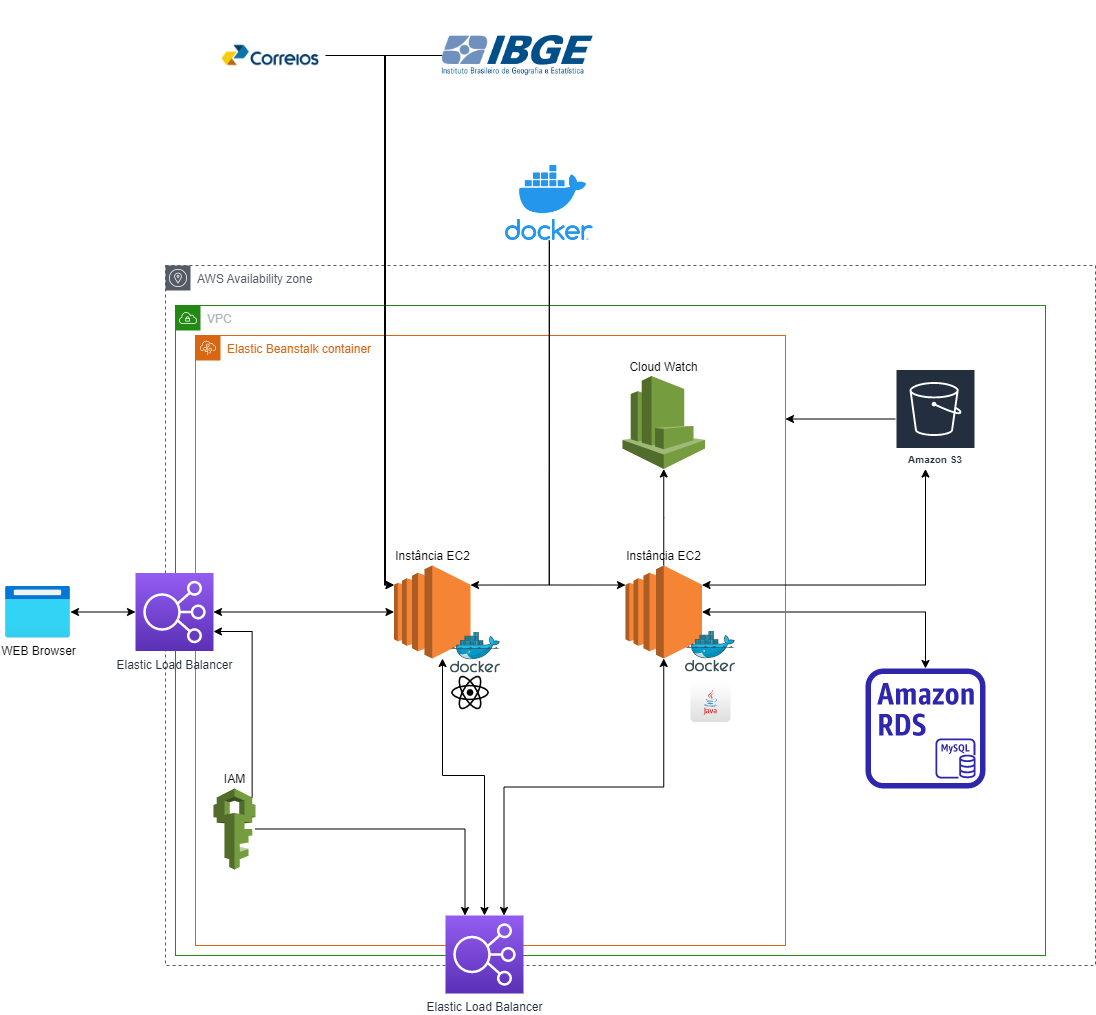
\includegraphics[width=0.65\textwidth]{images/ArquiteturaAplicacao_v6.png}
            \label{fig:infra3}
        \end{figure}
        
        \subsubsection{Elastic Load Balancing}
        
            Serviço que distribui o tráfego externo à infra estrutura entre instâncias de processamento da aplicação. Em diversos cenários de aplicações, a tecnologia permite que uma solução seja escalável de forma horizontal para um numero de instâncias de tamanhos variáveis de acordo com a parametrização do gestor da solução \citeonline{eld}.
        
        \subsubsection{Docker Container}

            Tecnologia que isola o ambiente da aplicação através da segregação de recursos em namespaces e imagem de aplicação, permitindo maior liberdade no uso dos recursos computacionais de execução em ambiente isolado e portabilidade \citeonline{docker}.
            
            Normalmente toma como ponto de partida a distribuição Alpine Linux, que tem o objetivo de ter apenas os recursos necessários para o sistema operacional, aumentando o controle do desenvolvedor sobre os utilitários do sistema operacional.
    
            Para a aplicação \emph{back end}, será empregada uma imagem baseada na pilha Amazon, Linux e Amazon Corretto 17.
            
        \subsubsection{AWS Elastic BeanStalk}

            Serviço gerenciado que abstrai a necessidade de tomar decisão sobre recursos físicos da aplicação, provisionando máquina e serviços necessários para a implementação da solução. Provê suporte à tecnologia Docker \emph{container} \citeonline{elbean}.
            
        \subsubsection{Amazon ECR - Amazon Elastic Container Registry}
        
            Similar ao serviço Docker Hub, é um serviço de armazenamento e registro de imagens de containers gerenciado pelo provedor AWS. Permite que seja possível realizar implantações (\emph{deploy}) automatizados a partir da atualização da imagem Docker armazenada no diretório em nuvem \citeonline{ecr}.

        \subsubsection{AWS RDS (Relational Database Service) - Amazon AWS}

            Serviço gerenciado que provê banco de dados com redundância em infraestrutura abstraída, suporta implementações de banco de dados relacionais: Amazon Aurora, MySQL, MariaDB, PostgreSQL, Oracle e Microsoft SQL Server. Disponibiliza as funcionalidades de uso mais recorrentes por aplicações \citeonline{rds}.
            
            Para a implementação da solução, identificou-se que o uso de uma instância MySQL se enquadra melhor às necessidades da aplicação por não existir necessidade imediata de atender altos volume de transações com o banco de dados.
            
        \subsubsection{Amazon S3}
        
            Serviço de armazenamento de objetos (no caso da Certvet, documentos de resultado de exames) que oferece escalabilidade \citeonline{s3}. 

    \section{Tecnologias de Desenvolvimento}
    
        Aproveitando da maturidade de \emph{frameworks} e bibliotecas \emph{front-end} e a complexicidade adicional do desenvolvimento de aplicações dedicadas para ambientes \emph{desktop} e móveis, com ênfase em celulares (necessidade de permissão de máquina para instalação e configuração da aplicação em ambiente heterogêneo além de particularidades pontuais de cada cliente), o foco da aplicação foi voltado para a plataforma WEB (navegadores \emph{desktop} e móveis).
        
        Para prototipação, foi utilizada a ferramenta Figma, um editor colaborativo \emph{online} de \emph{design} gráfico que permite a criação de interfaces de usuário. A ferramenta auxilia desenvolvedores a construir telas coesas e baseadas nos conceitos e práticas de \emph{User Experience} (UX) e \emph{User Interface }(UI). Como ferramenta de desenvolvimento, a plataforma GitHub será usada como principal ferramenta de versionamento dos  repositórios do projeto.
        
        Com o objetivo de facilitar o processo de implementação de uso da ferramenta nos estabelecimentos dos usuários, a instalação de um software como aplicação \emph{desktop} poderia influenciar negativamente à adoção da aplicação. Ainda, de acordo com as habilidades técnicas dos membros da equipe, foi optado por utilizar tecnologias web baseadas em servidores de aplicação remotos e gerenciados, oferecendo o software como serviço (\emph{Software as a Service - SaaS}).
        
        A oferta de software como serviço permite que atualizações e correções sejam implementadas mais rapidamente por não depender da interferência em infraestrutura de responsabilidade do cliente. Adicionalmente, reduz-se o risco de instalação do serviço de forma inadequada.

    \subsection{\emph{Front-end}}
    
        A pilha de tecnologias de desenvolvimento para o \emph{front-end} se concentram nas ferramentas e tecnologias:
        
        \begin{itemize}
        
            \item Figma: Editor colaborativo \emph{online} de \emph{design} gráfico que permite a criação de interfaces de usuário e que ajudará os desenvolvedores a construir telas coesas e baseadas nos conceitos e práticas de \emph{User Experience} (UX) e \emph{User Interface} (UI).\citeonline{figma}
        
            \item Typescript:
                Linguagem que permite programação fortemente tipada de código aberto desenvolvida pela Microsoft lançada em 1 de outubro de 2012. \citeonline{ts}
    
                É também um supertipo da linguagem  JavaScript, o que significa que possui todas as funcionalidades do JavaScript e além da adição de novos recursos. 
                
                Essa linguagem foi selecionada para desenvolver o \emph{front end} devido à complexidade e escala da aplicação, que requer estruturas de dados mais complexas do que o JavaScript pode oferecer suporte, fazendo-se necessário a utilização de uma linguagem com tipagem de dados forte. 
                
                Outro motivo que colaborou para a escolha foi a segurança, já que graças a tipagem de dados, erros que podem causar vulnerabilidades e passam despercebidos em aplicações desenvolvidas com JavaScript serão identificados no momento da compilação do TypeScript para JavaScript.
            
            \item SCSS:
                Linguagem de estilização para WEB compilada para CSS.
    
                Essa linguagem foi selecionada para estilizar o \emph{front end} da aplicação pelo fato de possuir compatibilidade com o CSS e também uma melhor estrutura organizacional de código quando comparado com o CSS.\citeonline{scss}
        
            \item ReactJS:
                Biblioteca JavaScript/TypeScript desenvolvida pelo Facebook para a criação de interfaces WEB lançada em 29 de maio de 2013. O React foi escolhido graças a arquitetura baseada em componentes que permite a reutilização dos mesmo em diferentes partes da aplicação. Os componentes são escritos utilizando JSX que possui uma sintaxe semelhante ao HTML, o que o torna fácil de utilizar.\citeonline{reactjs}
        
            \item Bootstrap:
                \emph{Framework front-end} que fornece estruturas de CSS para a criação de sites e aplicações responsivas de forma rápida e simples.\citeonline{bootstrap}
    
                Essa tecnologia foi escolhida pelo fato de reduzir consideravelmente o tempo de desenvolvimento da estilização da interface da aplicação com om usuário.
        
        \end{itemize}
    
        \subsection{\emph{Back-End}}
    
            Para compor a pilha de tecnologias aplicadas no \emph{back-end}, foi definido utilizar as seguintes tecnologias:
    
            \begin{itemize}
                \item Java 17: 
                    Linguagem de programação fortemente tipada com ênfase no paradigma de desenvolvimento orientado a objeto. Habitualmente empregada em aplicações comerciais e cientificas maduras, tanto open source como privadas.\citeonline{java}
    
                    A partir da comunidade de desenvolvimento, projetos open source de permissionamento livre permite acesso a bibliotecas e ferramentas como \emph{framework} Demoiselle, para assinatura de documentos que cumprem a especificação ICP-Brasil.
                    
                    A versão 17 é uma versão LTS - Long Term Service, permite o emprego das tecnologias e funcionalidades mais recentes da linguagem, sem prejuízo às implementações mais antigas.
        
                \item \emph{Framework}Spring Boot: 
                   \emph{ Framework} comumente utilizado da linguagem Java para aplicações de uso geral, permite integração sem quebras entre dependências de bibliotecas e frameworks especializados como Spring MVC, hibernate ou Apache Kafka \citeonline{spring}.
                    \begin{itemize}
                        \item ORM - spring JPA (Hibernate)
                        \item Spring Web - \emph{controllers}
                        \item Apache Tomcat - Servidor HTTP
                        \item Hibernate Validator
                        \item Mockito - \emph{Framework} que auxilia o desenvolvimento de testes de unidade
                        \item SL4J - \emph{Framework} dedicado ao registro de \emph{logs}
                    \end{itemize}
                \item SGBD MySQL:
                    Sistema de gerenciamento de banco de dados relacional com ampla implementação de provedores de tecnologias em nuvem aberta ou on premisses, tendo licença permissiva de uso e familiaridade aos membros da equipe.

                \item Postman:
                Ferramenta que permite realizar solicitações HTTP e requisições a fim de testar a API a partir de análises de suas respostas. Além disso, permite a depuração de testes de forma mais facilitada e a realização de testes de automação, auxiliando na garantia do funcionamento esperado por parte da API. 

                \item Swagger:
                \emph{Framework} que promove a organização das rotas através de documentações e geração de códigos cliente e servidor, seja de forma automática ou manual, \citeonline{swagger}.

            \end{itemize}
    
        \subsection{Ferramentas de testes automatizados}
        
            Com o objetivo de testar a aplicação e também garantir que as funções retornem os resultados esperados de forma a garantir a integração das partes da mesma, teste unitários são fundamentais para alcançar esses objetivos. Portanto, a equipe utilizará as ferramentas de testes automatizados listados a seguir:
            
            \begin{itemize}
                \item Jest: é um \emph{framework} de testes para JavaScript/TypeScript desenvolvido a partir do \emph{framework}Jasmine, também para testes automatizados.
                \item JUnit: é um \emph{framework} open-source de teste para a linguagem Java desenvolvido por Erich Gamma e Kent Beck. é assumido por padrão pelo \emph{framework} Spring e suas ferramentas (Spring Boot).
            \end{itemize}

%\subsection{Integrações existentes}

    %O sistema utiliza integração com a API dos Correios para preenchimento automático do endereço após a inserção do código de CPF do usuário, otimizando a experiência deste.
    

    \section{Manutenibilidade}
    Visando garantir boa resposta dos clientes, atingindo um elevado nível de qualidade, torna-se necessário estabelecer determinados requisitos e parâmetros de manutenibilidade e ferramentas que possam auxiliar esse processo. Partindo desses critérios, é possível mensurar o quanto o desenvolvimento do sistema apresenta conformidade com as boas práticas e, consequentemente, na qualidade do projeto.

        \subsection{\emph{Code Convention}}
        Buscando facilitar o fluxo de trabalho com um maior nível de legibilidade para todos os envolvidos no desenvolvimento do código e, consequentemente, simplificar a integração entre as diferentes partes do que está a ser desenvolvido, a equipe optou por adotar uma convenção de código. Visando o desenvolvimento de um código consistente e transparente, a convenção permite que os diferentes membros possam adicionar contribuições sem grandes dificuldades, aumentando a taxa de transferência e diminuindo o tempo de entrega, resultando em uma base de código mais uniforme e consequentemente impactando na facilidade da manutenção do código.

        \subsubsection{Codificação geral}
        A convenção adotada para a parte mais generalizada do código, é a mais comumente usada para o desenvolvimento utilizando a linguagem Java, sendo relativamente próxima dos padrões adotados em outras linguagens populares como JavaScript e Python. As regras seguem como base as sugestões de \emph{Coding Convention }da Oracle, mas foram adaptadas para as necessidades da equipe:

        \begin{itemize}
            \item
            Declaração de atributos e variáveis em português.
            \item
            Nomes de atributos e váriaveis devem ser redigidos em camelCase.
            \item
            Variáveis declaradas próximas de onde são inicializadas.
            \item
            Declarações globais preferencialmente no início do arquivo.
            \item
            Uso reduzido de variáveis, funções e objetos globais.
            \item
            Métodos nomeados com camelCase e prefixados com verbo em inglês que deixe claro o que o método faz.
            \item
            As constantes devem utilizar notação Upper case, utilizando underscore para separação das palavras em caso de nome composto.
            \item
            Nomes de classes e interfaces redigidos em PascalCase.
        \end{itemize}

    Somando-se a isso, a resolução do \emph{back-end} é dividida em pacotes para melhor distribuição e visibilidade da mesma. Sendo eles, o pacote \emph{model} contendo as classes de modelo, também usadas como entidades mapeadas do banco de dados, o pacote \emph{controller} contendo o gerenciamento da lógica do negócio através dos controladores e \emph{endpoints} do serviço, o pacote \emph{service} contendo a implementação da lógica de negócio através dos serviços e o pacote \emph{repository} para centralizar as regras de armazenamento dos \emph{beans} de entidade no sistema.

    \subsubsection{\emph{Commits}}
    A equipe optou por adotar os prefixos gerados pelo Jira, ferramenta utilizada para o gerenciamento de tarefas, para nomear as \emph{branchs} que serão commitadas tanto no \emph{front-end} quanto no \emph{back-end}.

    ERI-X: sendo ERI o prefixo base gerado pelo Jira e X o número de identificação daquela tarefa no \emph{dashboard}.

    Somado à padronização, fora adotada a prática de efetuar \emph{ pull requests} e o \emph{code review} por parte de um outro integrante do time, evitando que uma implementação ou alteração seja adicionada diretamente na \emph{branch} principal do repositório.

    \subsection{\emph{Design Patterns} e boas práticas}
    Visando a padronização do projeto, o time adotou dois padrões comumente usados pela comunidade de desenvolvedores: \emph{Design Patterns} e \emph{Facade,} sendo este último adotado pensando na redução do acoplamento entre as diferentes camadas do projeto e na diminuição da complexidade da API e o padrão \emph{Builder} para isolar a complexidade da criação dos objetos, facilitando a criação das diferentes implementações, todas baseadas em uma mesma interface.

    \subsubsection{\emph{Clean Code}}
    Somado ao \emph{Code Convention} abordado anteriormente, o \emph{Clean Code} é um conjunto de práticas de desenvolvimento a fim de garantir que o código seja legível para todos e que, consequentemente, implique em uma manutenção mais ordenada e simplificada, evitando gargalos tendo em vista que propaga maior inteligibilidade por parte dos desenvolvedores. As práticas adotadas pela equipe podem ser lidas abaixo:

    \begin{itemize}
        \item 
        Definição significativa dos nomes de classes, atributos, métodos, objetos e variáveis.
        \item
        Uso de ENUM e constantes para padronização de números que façam sentido no código.
        \item
        Criação de funções simples, de procedimentos transparentes e pequenas.
        \item
        Uso reduzido de comentários que não sejam necessários.
        \item
        Evitar a redundância e a repetição de código.
        \item
        Reduzir ao máximo as dependências, de forma a aumentar o desacoplamento e a independência entre as partes do projeto.
        \item
        Realizar o tratamento de erros para garantir que o código continuará fazendo o que foi programado para fazer.
        \item
        Cobrir e validar todos os processos sensíveis e importantes com testes limpos.
    \end{itemize}

    \subsubsection{SOLID}
    O conjunto de cinco princípios básicos, denominado na área por SOLID, tem como principal objetivo garantir a maior qualidade no processo de desenvolvimento de software, resultando em uma aplicação mais fácil de ser testada, mantida, corrigida, considerando-se a flexibilidade gerada no código em se adequar às possíveis mudanças e até mesmo escalada \citeonline{solid1}. No que tange ao entendimento da equipe sobre os princípios e como os mesmos serão aplicados no projeto:

    \begin{itemize}
        \item 
        \emph{Single Responsability Principle} (SRP), o princípio da responsabilidade única, basicamente determina que uma classe deve ter simplesmente um único motivo para existir, uma única responsabilidade.
        \item 
         \emph{Open-closed Principle} (OCP), ou princípio aberto-fechado, o segundo princípio prevê que uma entidade deve ser aberta para a extensão e fechada para a modificações.
        \item 
        \emph{Liskov Substitution Principle} (LSP), o terceiro
        princípio, o de substituição de Liskov, determina que uma classe que seja derivada deve ser substituível por sua classe originária \citeonline{solid2}.
        \item 
        \emph{Interface Segregation Principle} (ISP), o princípio da segregação da interface prevê que uma classe não deve implementar interfaces que possuem atributos e métodos que ela não utilizará.
        \item 
        \emph{Dependency Inversion Principle} (DIP), o quinto princípio, o da inversão de dependência determina que uma classe deve sim depender de abstrações, no entanto, jams depender de implementações \citeonline{solid2}.
    \end{itemize}

        \subsection{\emph{Logs}}
        A fim de monitorar o sistema em tempo real de execução, principalmente no que tange à camada do servidor, o time adotou o \emph{CloudWatch Logs}, ferramenta da Amazon para visualização destes, tornando possível o monitoramento do estado dos objetos. Através de diferentes registros como: \emph{info, warn, debug e error,} a equipe tem a sua disposição insumos para consultar os dados de \emph{log}da aplicação, monitorar os \emph{logs}de instâncias do Amazon EC2 e arquivá-los com segurança para futuras análises, quando necessário, de forma que, quando ocorrer falha do sistema, um \emph{log} poderá ser consultado para devidas identificações, análises e resoluções.

    
    \section{Segurança}
    
        A aplicação, por tratar dados pessoais que podem identificar indivíduo, precisa utilizar métodos seguros e que cumpram regulamentação legal e específica como parte dos requisitos.
    
        \subsection{Comunicação}
        
            A aplicação utiliza interfaces de aplicação de transferência representacional de estado (REST API), tomando como base o protocolo HTTP.
        
            O protocolo \emph{Hyper Text Transfer Protocol} (HTTP) realiza comunicação através de interfaces da arquitetura cliente-servidor. Tanto nos modelos conceituais TCP/IP e \emph{Open System Interconnection} (OSI) está compreendido pela camada de aplicação \citeonline{PetersonRedes}.
        
            Por permitir comunicação na arquitetura cliente-servidor sem criptografia (trafega dados através de texto simples pelas das camadas de rede), é considerado uma forma não segura de troca de dados.
            
            Para que a comunicação possa ocorrer sem perda de dados ou interceptação entre as partes, é necessário adicionar criptografia \emph{Transport Layer Security} (TLS) ou \emph{Secure Socket Layer} (SSL), base do TLS na comunicação ponto a ponto, estendendo o protocolo para \emph{Hyper Text Transfer Protocol} Secure (HTTPS) \citeonline{PetersonRedes}.
            
        \subsection{Privacidade}
        
            Em diversos sistemas, tanto \emph{mobile como web,} diversas informações são trocadas entre o usuário e o servidor a todo instante. Dentre essas informações é possível destacar documentos pessoais, senhas e informações sigilosas. Visto isso, uma das prioridades do sistema a ser desenvolvido será a privacidade de seus usuários e de suas informações.
        
            A lei 13.709/2018, conhecida como Lei Geral de Proteção de Dados Pessoais (LGPD) foi concebida com intuito de disciplinar o uso de dados pessoais por instituições, empoderando a pessoa física sobre os direitos fundamentais da liberdade e privacidade sobre seus dados \citeonline{lgpd}.
            
            A lei dispõe sobre atividades em que ocorra "tratamento de dados". Como explica o tribunal de justiça de São Paulo (TJ-SP):
            
            \begin{citacao}
                Considera-se “tratamento de dados” qualquer atividade que utilize um dado pessoal na execução da sua operação, como, por exemplo: coleta, produção, recepção, classificação, utilização, acesso, reprodução, transmissão, distribuição, processamento, arquivamento, armazenamento, eliminação, avaliação ou controle da informação, modificação, comunicação, transferência, difusão ou extração.
            \end{citacao}
            
            Tanto a Serpro quanto o TJ-SP relatam que a lei prevê três agentes das instituições, listando suas respectivas responsabilidades principais:
            
            \begin{citacao}
                Controlador: Responsável pelas decisões relativas ao tratamento dos dados
                Operador: Delegado pelo Controlador, operacionaliza as decisões do Controlador
                Encarregado: Atender às demandas dos titulares, interagir com a autoridade nacional de proteção de dados (ANPD) e orientar funcionários e contratados sobre as práticas de proteção de dados.
            \end{citacao}
            
            O titular dos dados é aquele que pode ter dados que identificam a pessoa natural, sendo tratados , distribuídos ou armazenados. Para que os dados possam ser armazenados nos termos da lei, é necessário que exista expressa autorização pelo titular dos dados, devidamente armazenados para fins de fiscalização. A distribuição indevida desses dados poderá acarretar ônus ao propagador. \citeonline{lgpdComoCumprir}
            
            Portanto, o mapeamento dos dados necessários para as atividades previstas pela aplicação e armazenamento de dados sensíveis é um ponto de atenção para ser considerado desde o desenvolvimento da modelagem de dados, passando pelo trânsito dos dados até a comunicação com os usuários que realizarão interação com a ferramenta.
            
            Nesse sentido, foi identificada a necessidade de avaliar a utilização de criptografia e autenticação em todas as etapas de trânsito de dados e armazenamento de banco de dados.
    
        \subsection{Autenticação JWT}
    
            JSON \emph{Web Token} (JWT) é um padrão de indústria para autenticação e troca de informações. Ele é um formato baseado em texto e amplamente aceito por diversas linguagens, visto a utilização do JSON como base. JWT é um dos elementos do JSON \emph{Object Signing and Encryption} (JOSE). Outros elementos do JOSE são o JSON \emph{Web Encryption} (JWE), que é o responsável pela criptografia para a assinatura do \emph{token}, o JSON \emph{Web Algorithms} (JWA), responsável pelo algoritmo, o JSON \emph{Web Keys} (JWK), correspondente as chaves para a assinatura e, por fim, o JSON \emph{Web Signature} (JWS), que consiste na assinatura do token, enquanto o JWT é o \emph{token} em si, \citeonline{jwt}.
            
            O JWT tem como objetivo realizar a autenticação entre duas partes por meio de um \emph{token} assinado que autentica uma requisição Web. O \emph{token} é um código, uma chave ou uma cadeia de caracteres que armazenam objetos JSON com os dados que permitirão a autenticação da requisição.
            Em um sistema no qual o cliente deseja se autenticar, o cliente enviará na requisição seus dados de autenticação como o e-mail e a senha. Após o sistema ter verificado que os dados do cliente estão corretos, o servidor criará um \emph{token} para o cliente. Com esse \emph{token}, o cliente terá condições de acessar na aplicação informações nas quais este não conseguia, visto que ainda não havia se autenticado. 
            
            O JWT é composto por três componentes, sendo eles denominados de “\emph{Header}”, “\emph{Payload}” e “\emph{Signature}”. O “\emph{Header}” pode ser descrito como o cabeçalho do \emph{token} e possui dois campos, sendo o primeiro campo denominado “alg”, que indica qual o algoritmo de criptografia usado, enquanto o outro campo, chamado “typ”, tem como objetivo indicar que se trata de um \emph{token} JWT. \citeonline{jwt}
            O componente chamado de “Payload” carrega os dados referentes a autenticação. Nesse segmento pode-se diversos campos como “exp” que indica o tempo de expiração do JWT, “sub” que informa o assunto do \emph{token}, “aud” que identifica quem deverá receber os dados do JWT, “iat” que identifica o tempo de existência do \emph{token}, entre outros campos.\citeonline{jwt}
            
            Por fim, o componente “\emph{Signature}” é a assinatura única de cada \emph{token} que é gerada a partir de um algorito de criptografia e tem seu corpo com base no \emph{“Header”, “Payload”} e no segredo definido pela aplicação. Em outras palavras, o “\emph{Signature}” é a codificação do \emph{“Header”, “Payload”} junto com uma palavra-chave.
            
            O \emph{token} é uma chave de acesso assinada digitalmente e garante segurança e confiabilidade. Como os \emph{tokens} são assinados, é possível o servidor verificar a legitimidade do \emph{token}, visto que esse carrega consigo a informação de sua origem. O \emph{token} completo consiste na junção dos três componentes separados única e exclusivamente por um ponto. Sendo assim, após a assinatura realizada, o  \emph{token} estará pronto. 
            
            Com o \emph{token} codificado é impossível decodificar a assinatura deste sem que haja o segredo-chave da aplicação. Entretanto, havendo o segredo, o \emph{token} poderá ser facilmente decodificado e verificado sua validade. 
            
            O JWT tem muita notoriedade por ser uma forma extremamente segura de compartilhamento de informações e autenticação de usuários. Ele é compacto, completo e fácil de se utilizar, além de ser aceito por diversas linguagens. Toda a informação necessária para a autenticação e autorização de acesso consta no \emph{token}, isso significa que a requisição será atendida independentemente do servidor. Com o JWT é possível ter escala em performance, visto a necessidade do servidor de apenas calcular o \emph{hash}, sem buscar nenhuma informação em alguma base ou tabela. Outro lado positivo na utilização do JWT é que é possível ter diversos servidores rodando em domínios diferentes e todos utilizando o mesmo \emph{token}.
            
            O lado negativo do JWT está baseado em sua chave secreta. Se essa chave for em algum momento exposta, algum indivíduo mal intencionado poderá ter acesso aos dados ali armazenados.

    
        \subsection{Legislação}
        
            Sendo uma aplicação desenvolvida para área de medicina veterinária, devem ser observadas legislações e decretos concernentes.
        
            \begin{itemize}
            
                \item O projeto exigirá login com CRMV para acessar áreas privativas dá área de medicina veterinária. Código de Ética Profissional do Médico-Veterinário, capítulo 5°, Art. 9°. \citeonline{manual}.
                
                \item Será obrigatória a correlação da clínica com o médico-veterinário responsável. Norma Técnica Especial Art. 3°. \citeonline{manual}.
                
                \item Os métodos de eutanásia disponíveis no preenchimento das informações do sistema. Resolução CFMV Nº 1.000, de 11 de Maio de 2012, Art. 14, anexo 1. \citeonline{manual}.
                
            \end{itemize}
        
        \subsection{Regulamentação}
        
            Tendo em vista a seriedade dos procedimentos com os quais o profissional veterinário lida no seu dia a dia e que são parte do escopo da aplicação, o Código de Ética do Médico-Veterinário com a Resolução CFMV nº 1138, publicada no Diário Oficial da União em 25/01/2016, deve ser seguido como instrumento normativo referencial para todo o fluxo de exercício profissional, assegurando que a CertVet esteja em conformidade com os princípios fundamentais da profissão, deveres profissionais, direito dos médicos veterinários, responsabilidade e comportamento do profissional e honorários profissionais, além da relação com o cidadão consumidor de seus serviços, com o animal, o meio ambiente e também com a justiça.  \citeonline{etica}

    \section{Viabilidade Financeira}
    
        A arrecadação de fundos do projeto se baseia em duas obrigações do CFMV: A formalização de atos médicos usando um termo de consentimento livre e esclarecimento, e o armazenamento da maioria destes por um tempo mínimo de dois anos.

        \subsection{Serviços utilizados}
        
            Os serviços da provedora de nuvem foram considerados com base em custos sem pagamento antecipado ou reserva de recursos. Essa estimativa considera cenário real de armazenamento de dados e processamento da aplicação no Brasil, cumprindo com leis de privacidade de dados. Demais serviços acessórios como armazenamento de \emph{logs}e dados de código da aplicação podem ser armazenados fora do país.

            \begin{itemize}
            
                \item Amazon CloudWatch: 1.21 USD/mês em US East (N. Virginia) Standard Logs: Data Ingested (2 GB), Number of Dashboards (1), Number of Standard Resolution Alarm Metrics (2)
                
                \item Amazon EC2: 13.44 USD/mês em South America (Sao Paulo) Computing: Operating system (Linux), Quantity (1), Pricing strategy (EC2 Instance Savings Plans 1 Year No Upfront), Storage amount (30 GB), Instance type (t2.micro)
                
                \item Amazon RDS for MySQL: 34.97 USD/mês em South America (Sao Paulo) Database Services: Storage for each RDS instance (General Purpose SSD (gp2)), Storage amount (30 GB), Quantity (1), Instance type (db.m1.small), Utilization (On-Demand only) (50\% Utilized/Month), Deployment option (Single-AZ), Pricing strategy (OnDemand), Additional backup storage (30 GB)
                
                \item Amazon Simple Storage Service (S3): 0.09 USD/mês em US East (N. Virginia) Storage: S3 Standard storage (4 GB per month)
                
                \item Elastic Load Balancing: 30.32 USD/mês em South America (Sao Paulo) Load Balancer: Number of Application Load Balancers (1)
                
            \end{itemize}
    
    
            Assim, os custos estimados de serviços ficou em USD 80.03 mensais, que podem ser visto no link: \url{https://github.com/EquipeRocketIFSP/Documentos/blob/main/DesenhoAplicacao/Viabilidade\%20Financeira\%20Custos\%20de\%20Infraestrutura\%20-\%20AWS\%20Pricing\%20Calculator.pdf}. Na Tabela \ref{custo_infraestrutura1} temos uma visualização do custo mensal, de acordo com as projeções iniciais de uso do sistema, que deve ser revisada com o aumento de demanda.
        
            \begin{table*}[h]
                    % \centering
                     \caption{Custo mensal da infraestrutura do desenvolvimento}
                    \resizebox{\columnwidth}{!}{%
                    \begin{tabular}{|lrrr|r|}
                        \hline
                        \multicolumn{1}{|l|}{Custo}
                            & \multicolumn{1}{r|}{USD}
                            & \multicolumn{1}{r|}{Câmbio}
                            & \multicolumn{1}{r|}{R\$}
                            & Total \\ \hline
                        \multicolumn{1}{|l|}{Amazon CloudWatch}
                            & \multicolumn{1}{r|}{1,21}
                            & \multicolumn{1}{r|}{5,50}
                            & \multicolumn{1}{r|}{6,655}
                            & 6,66  \\ \hline
                        \multicolumn{1}{|l|}{Amazon EC2}
                            & \multicolumn{1}{r|}{13,44}
                            & \multicolumn{1}{r|}{5,50}
                            & \multicolumn{1}{r|}{74,592}
                            & 74,59 \\ \hline
                        \multicolumn{1}{|l|}{Amazon RDS for MySQL}
                            & \multicolumn{1}{r|}{34,97}
                            & \multicolumn{1}{r|}{5,50}
                            & \multicolumn{1}{r|}{192,335}
                           & 192,34  \\ \hline
                        \multicolumn{1}{|l|}{Amazon Simple Storage Service (S3)}
                            & \multicolumn{1}{r|}{0,09}
                            & \multicolumn{1}{r|}{5,50}
                            & \multicolumn{1}{r|}{0,495}
                            & 0,50 \\ \hline
                        \multicolumn{1}{|l|}{Elastic Load Balancing}
                            & \multicolumn{1}{r|}{30,32}
                            & \multicolumn{1}{r|}{5,50}
                            & \multicolumn{1}{r|}{166,76}
                            & 166,76 \\ \hline
                        \multicolumn{4}{|l|}{Total de infraestrutura (Mês)}
                            & 440,85   \\ \hline
                    \end{tabular}%
                    }
               \label{custo_infraestrutura1}
                \centering
                \footnotesize Fonte: Elaborado pelos autores.
                \end{table*}
         
        \subsection{Tributação}
        
            % Impostos sobre serviços prestados com fato gerador ocorrido no município de São Paulo incide alíquota máxima para o imposto sobre serviço (ISS), incorrendo 5\% do valor de faturamento. Demais tributações dependerão do regime tributário a ser escolhido na constituição jurídica, não sendo prevista no momento da elaboração do projeto.

            Para formar o custo base de mão de obra, foi considerado o salário médio aproximado de desenvolvedores no Brasil de R\$ 4.000,00 \citeonline{glassdoor} . Para efeitos práticos, considerou-se os custos relacionados à folha de pagamento para 200\%, a partir da proposta de metodologia de mensuração do custo do trabalho no Brasil, que aproxima o custo em 183\% em pesquisa realizada em 2012 pelo Centro de Microeconomia Aplicada (C-Micro) da Fundação Getúlio Vargas/Escola de Economia de São Paulo (FGV/EESP) \citeonline{FGV}, como pode ser observado na Tabela \ref{tab:custos-maodeobra}.
 
          
        \subsection{Mão de obra}
        
            % Considerando a necessidade de remuneração dos envolvidos e importante medida para alcance do ponto de equilíbrio do negócio, foi considerada a seguinte remuneração mensal mínima com base nas atividades designadas de cada membro da equipe:

            % \begin{itemize}
            %     \item \emph{product Owner}: R\$ 1.200,00 + encargos de folha
            %     \item \emph{scrum Master}: R\$ 1.200,00 + encargos de folha
            %     \item Team Member: R\$ 1.200,00 + encargos de folha
            % \end{itemize}
            
            O cálculo das horas do projeto levou em consideração três tipos de requisitos funcionais a serem implementados, a saber, os níveis fácil, médio e difícil, categorizados de acordo com a experiência dos integrantes. Foi atribuído três dias para cada requisito fácil, cinco dias nos requisitos médios  dez dias para cada um dos requisitos difíceis, como mostra a figura 
            \ref{fig:maodeobra}.

Os custos com mão de obra dizem respeito ao período de desenvolvimento, quando todos os integrantes participam da implementação.

            \begin{table}[h]
                \centering
                 \caption{Custos de mão de obra mensal. Em R\$}
                \resizebox{12cm}{!}{%
                \begin{tabular}{|l|r|r|r}
                    \hline
                    \multicolumn{1}{|l|}{Colaborador}
                        & \multicolumn{1}{r|}{Valor}
                        & \multicolumn{1}{r|}{Quantidade}
                        & \multicolumn{1}{r|}{Total}
                        \\ \hline
                    \multicolumn{1}{|l|}{\emph{Product Owner}}
                        & \multicolumn{1}{r|}{12.000,00}
                        & \multicolumn{1}{r|}{1}
                        & \multicolumn{1}{r|}{12.000,00}
                        \\ \hline
                    \multicolumn{1}{|l|}{\emph{Scrum} Master}
                        & \multicolumn{1}{r|}{12.000,00}
                        & \multicolumn{1}{r|}{1}
                        & \multicolumn{1}{r|}{12.000,00}
                        \\ \hline
                    \multicolumn{1}{|l|}{Team Member}
                        & \multicolumn{1}{r|}{8.000,00}
                        & \multicolumn{1}{r|}{5}
                        & \multicolumn{1}{r|}{40.000,00}
                        \\ \hline
                \end{tabular}%
                }
               
                \label{tab:custos-maodeobra}
                \centering
                \footnotesize Fonte: Elaborado pelos autores.
            \end{table}

            % Considerando que os encargos de folha são frequentemente aproximados a 100\% do valor bruto da remuneração, foi aplicado essa regra geral para facilitar o cálculo.
            
            % Portanto, os custos de remuneração são de aproximadamente R\$ 36.000,00.
            
            \begin{figure}[H]
                \centering
                \caption{Mão de obra mensal}
                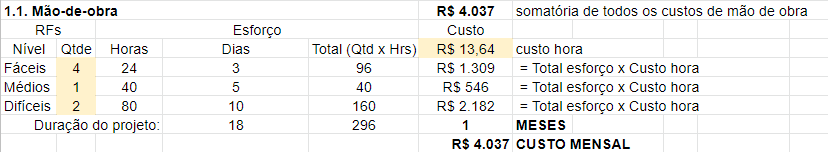
\includegraphics[width=1\textwidth]{images/Mao-de-obra.png}
                
                \label{fig:maodeobra}
                \centering
                \footnotesize Fonte: Elaborado pelos autores.
            \end{figure}
   \begin{itemize}
      \item Custo-base: R\$ 8.000,00 
        \item Dias-base: 22 | Dia-hora: 8
         \item Custo-hora R\$ 45,45
   \end{itemize}
             
           

        % \subsection{Destino dos Custos}
        
        %     Considerando as funcionalidades do projeto e o número de colaboradores, foram distribuídas tarefas para contabilizar as horas do projeto.

        %     \begin{table*}[h]
        %         % \centering
                
        %         \resizebox{\columnwidth}{80}{%
        %         \begin{tabular}{|lrrr|r|}
        %             \hline
        %             \multicolumn{1}{|l|}{Funcionalidade}                & \multicolumn{1}{r|}{Dias de Trabalho}
        %                 & \multicolumn{1}{r|}{Membros Atuando}
        %                 & \multicolumn{1}{r|}{Horas Totais}
        %                 &  Custo \\ \hline
        %             \multicolumn{1}{|l|}{Módulo de autenticação}
        %                 & \multicolumn{1}{r|}{3}
        %                 & \multicolumn{1}{r|}{2}
        %                 & \multicolumn{1}{r|}{48} 
        %                 & R\$ 654,55  \\ \hline
        %             \multicolumn{1}{|l|}{Agendamento online}           & \multicolumn{1}{r|}{3}
        %                 & \multicolumn{1}{r|}{2}
        %                 & \multicolumn{1}{r|}{48} 
        %                 & R\$ 654,55  \\ \hline
        %             \multicolumn{1}{|l|}{Prontuário clínico digital}
        %                 & \multicolumn{1}{r|}{10}
        %                 & \multicolumn{1}{r|}{6}
        %                 & \multicolumn{1}{r|}{480} 
        %                 & R\$ 6.545,45  \\ \hline
        %              \multicolumn{1}{|l|}{Registro de alterações assinadas digitalmente}
        %                 & \multicolumn{1}{r|}{10}
        %                 & \multicolumn{1}{r|}{3}
        %                 & \multicolumn{1}{r|}{240} 
        %                 & R\$ 3.272,73  \\ \hline
        %             \multicolumn{1}{|l|}{Gerenciamento de medicação}
        %                 & \multicolumn{1}{r|}{5}
        %                 & \multicolumn{1}{r|}{3}
        %                 & \multicolumn{1}{r|}{120} 
        %                 & R\$ 1.636,36  \\ \hline
        %             \multicolumn{1}{|l|}{Mapeamento Genealógico}
        %                 & \multicolumn{1}{r|}{3}
        %                 & \multicolumn{1}{r|}{3}
        %                 & \multicolumn{1}{r|}{72} 
        %                 & R\$ 981,82  \\ \hline
        %             \multicolumn{1}{|l|}{Controle de vacinação}
        %                 & \multicolumn{1}{r|}{3}
        %                 & \multicolumn{1}{r|}{3}
        %                 & \multicolumn{1}{r|}{72} 
        %                 & R\$ 981,82  \\ \hline
        %             \multicolumn{3}{|l|}{Total}
        %                 & \multicolumn{1}{r|}{1080}
        %                 & R\$ 14.727,27     \\ \hline
        %         \end{tabular}%
        %         }
        %         \caption{Destinação dos custos de desenvolvimento}
        %         \label{tab:custos_func}
        %     \end{table*}

        \subsection{Custos de Operação}
        
            Após o período de desenvolvimento, os custos para manter o projeto se devem exclusivamente à mensalidade dos servidores e da remuneração do Team Member responsável. Os custos totais podem ser observado na Tabela \ref{tab:custos-maodeobra}.


            \begin{table*}[ht]
            \caption{Custos Totais Estimados}
    \resizebox{\columnwidth}{!}{%
    \begin{tabular}{|lrrrr|r|}
        \hline
        \multicolumn{1}{|l|}{Custo}                              & \multicolumn{1}{r|}{USD}   & \multicolumn{1}{r|}{Câmbio} & \multicolumn{1}{r|}{R\$}       & Quantidade & Total                            \\ \hline
        \multicolumn{1}{|l|}{Amazon CloudWatch}                  & \multicolumn{1}{r|}{1,21}  & \multicolumn{1}{r|}{5,50}   & \multicolumn{1}{r|}{6,655}     & 1          & 6,66                            \\ \hline
        \multicolumn{1}{|l|}{Amazon EC2}                         & \multicolumn{1}{r|}{13,44} & \multicolumn{1}{r|}{5,50}   & \multicolumn{1}{r|}{74,592}    & 1          & 74,59                           \\ \hline
        \multicolumn{1}{|l|}{Amazon RDS for MySQL}               & \multicolumn{1}{r|}{34,97} & \multicolumn{1}{r|}{5,50}   & \multicolumn{1}{r|}{192,335}   & 1          & 192,34                          \\ \hline
        \multicolumn{1}{|l|}{Amazon Simple Storage Service (S3)} & \multicolumn{1}{r|}{0,09}  & \multicolumn{1}{r|}{5,50}   & \multicolumn{1}{r|}{0,495}     & 1          & 0,50                            \\ \hline
        \multicolumn{1}{|l|}{Elastic Load Balancing}             & \multicolumn{1}{r|}{30,32} & \multicolumn{1}{r|}{5,50}   & \multicolumn{1}{r|}{166,76}    & 1          & 166,76                           \\ \hline
        \multicolumn{1}{|l|}{Team Member}                        & \multicolumn{1}{r|}{}      & \multicolumn{1}{r|}{}       & \multicolumn{1}{r|}{8.000,00}  & 1          & 8.000,00                        \\ \hline
        \multicolumn{5}{|l|}{Total Mensal}                                                                                                                                & 8.440,85                       \\ \hline
        \multicolumn{5}{|l|}{Total Anual}                                                                                                                                 & \multicolumn{1}{l|}{101.290,20} \\ \hline
    \end{tabular}%
    }

\label{tab:custos1}
\centering
\footnotesize Fonte: Elaborado pelos autores.
\end{table*}
    
        \subsection{Receitas}
            \begin{table}[H]
            \caption{Captação de Recursos}
                \resizebox{\columnwidth}{!}{%
                \begin{tabular}{| p{5cm}|l|l|l|}
                    \hline
                    \multicolumn{1}{|c|}{} & \multicolumn{1}{|c|}{\textbf{Plano Básico  R\$110,00/mês}}  & \multicolumn{1}{c|}{\textbf{Plano Premium  R\$ 165,00/mês}} \\ \hline
                    Agenda  &x &x \\ \hline
                    
                    Prontuário Clínico   &x &x\\ \hline
                    
                    Controle de Vacinação &x &x \\ \hline
                    
                    Gerenciador de Medicamentos &x &x \\ \hline
                    
                    Rastreio de Alterações &   &x  \\ \hline
                    
                    Histórico de Aspectos Hereditários &  &x \\ \hline
                \end{tabular}%
                }
            
            \label{tab:custos2}
            \centering
            \footnotesize Fonte: Elaborado pelos autores.
            \end{table}
            
            % \begin{figure}[H]
            %     \centering
            %     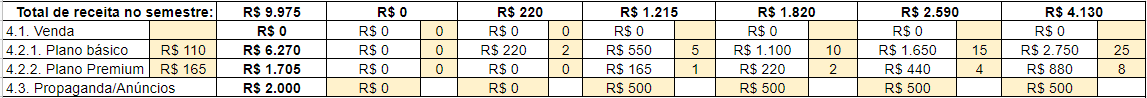
\includegraphics[width=1 \textwidth]{images/REALISTA.png}
            %     \caption{Cenário Realista}
            %     \label{fig:cenariorealista1}
            % \end{figure}
            % \begin{figure}[H]
            %     \centering
            %     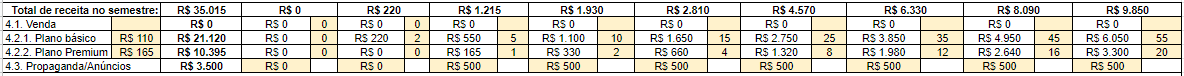
\includegraphics[width=1 \textwidth]{images/REALISA2.png}
            %     \caption{Versão Final do Cenário Realista}
            %     \label{fig:cenariorealista2}
            % \end{figure}
    
        \subsection{Gráficos dos Cenários}
        
            % Cenário Realista
            \begin{figure}[H]
                \centering
                 \caption{Primeira Versão do Cenário Realista}
                \includegraphics[width=1 \textwidth]{images/CenárioRealista.png}
               
                \label{fig:cenariorealistaGrafico1}
                \centering
            \footnotesize Fonte: Elaborado pelos autores.
            \end{figure}
            
            \begin{figure}[H]
                \centering
                \caption{Segunda Versão do Cenário Realista}
                \includegraphics[width=1 \textwidth]{images/CenárioRealista2.png}
                
                \label{fig:cenariorealistaGrafico2}
                \centering
            \footnotesize Fonte: Elaborado pelos autores.
            \end{figure}
            
            \begin{figure}[H]
                \centering
                \caption{Versão Final do Cenário Realista}
                \includegraphics[width=1 \textwidth]{images/CenárioRealista3.png}
                
                \label{fig:cenariorealistaGrafico3}
                \centering
            \footnotesize Fonte: Elaborado pelos autores.
            \end{figure}
            
            
            % Cenário Pessimista
            \begin{figure}[H]
                \centering
                \caption{Primeira Versão do Cenário Pessimista}
                \includegraphics[width=1 \textwidth]{images/CenárioPessimista.png}
                
                \label{fig:cenarioPessimistaGrafico}
                \centering
            \footnotesize Fonte: Elaborado pelos autores.
            \end{figure}
            
            \begin{figure}[H]
                \centering
                \caption{Versão Final do Cenário Pessimista}
                \includegraphics[width=1 \textwidth]{images/CenárioPessimista2.png}
                
                \label{fig:cenarioPessimistaGrafico1}
                \centering
            \footnotesize Fonte: Elaborado pelos autores.
            \end{figure}
            
            % Cenário Otimista
            \begin{figure}[H]
                \centering
                \caption{Primeira Versão do Cenário Otimista}
                \includegraphics[width=1 \textwidth]{images/CenárioOtimista.png}
                
                \label{fig:cenarioOtimistaGrafico}
                \centering
            \footnotesize Fonte: Elaborado pelos autores.
            \end{figure}
            
            
            \begin{figure}[H]
                \centering
                 \caption{Versão Final do Cenário Otimista}
                \includegraphics[width=1 \textwidth]{images/CenárioOtimista2.png}
               
                \label{fig:cenarioOtimistaGrafico2}
                \centering
            \footnotesize Fonte: Elaborado pelos autores.
            \end{figure}

    \section{Fases de entrega}
    
        O desenvolvimento do projeto foi dividido em três fases de entregas recorrentes, de forma que atendesse à demanda recebida por parte dos clientes. A primeira delas consiste na POC, a segunda a apresentação do MVP e, para finalizar, a Entrega Final. O Quadro \ref{tab:escopo} relaciona as principais funcionalidades da CertVet com a fase em que a sua implementação é esperada.
    
            \begin{quadro}[H]
                \centering
                \caption{Escopo do Projeto}
                \resizebox{\columnwidth}{!}{%
                \begin{tabular}{|lrrrr|r|}
                    \hline
                    \multicolumn{1}{|l|}{Funcionalidades}                              & \multicolumn{1}{r|}{POC}   & \multicolumn{1}{r|}{MVP} & \multicolumn{1}{r|}{Produto Final}                                   \\ \hline\multicolumn{1}{|l|}{Processo de login}                  & \multicolumn{1}{c|}{X}  & \multicolumn{1}{c|}{X}   & \multicolumn{1}{c|}{X}                                 \\ \hline
                    \multicolumn{1}{|l|}{Módulo de autenticação}                  & \multicolumn{1}{c|}{}  & \multicolumn{1}{c|}{X}   & \multicolumn{1}{c|}{X}                                 \\ \hline
                    \multicolumn{1}{|l|}{Agendamento online}                         & \multicolumn{1}{c|}{} & \multicolumn{1}{c|}{X}   & \multicolumn{1}{c|}{X}                               \\ \hline
                    \multicolumn{1}{|l|}{Prontuário clínico digital}               & \multicolumn{1}{r|}{} & \multicolumn{1}{c|}{X}   & \multicolumn{1}{c|}{X}                             \\ \hline
                    \multicolumn{1}{|l|}{Registro de alterações assinados digitalmente} & \multicolumn{1}{r|}{}  & \multicolumn{1}{r|}{}   & \multicolumn{1}{c|}{X}                                 \\ \hline
                    \multicolumn{1}{|l|}{Gerenciamento de medicação}             & \multicolumn{1}{r|}{} & \multicolumn{1}{r|}{}   & \multicolumn{1}{c|}{X}                               \\ \hline
                    \multicolumn{1}{|l|}{Histórico de aspectos hereditários}                      & \multicolumn{1}{r|}{}      & \multicolumn{1}{r|}{}       & \multicolumn{1}{c|}{X}                           \\ \hline
                    \multicolumn{1}{|l|}{Controle de vacinação}                       & \multicolumn{1}{r|}{}      & \multicolumn{1}{r|}{}       & \multicolumn{1}{c|}{X}                           \\ \hline                  
                \end{tabular}%
                }
            
            \label{tab:escopo}
            \centering
            \footnotesize Fonte: Elaborado pelos autores.
            \end{quadro}
        
        \subsubsection{Prova de Conceito}
        
            A Prova de Conceito, POC, consiste na comprovação de viabilidade técnica da arquitetura proposta, sem considerar implementação de lógica de negócios. Oferece ao cliente uma demonstração de que o produto pode ser desenvolvido, visualizando uma a ideia abstrata de como a aplicação se comporta. 

            Para a POC da CertVet, a equipe apresentou o desenho da arquitetura com as especificações propostas sendo um processo de cadastro de usuário e \emph{login} e regras de negócio simples implementadas no \emph{back-end}. Este processo teve a finalidade de demonstrar o trânsito dos dados através de chamadas com sucesso à API implementada no servidor com respostas previamente esperadas, demonstrando a comunicação entre as camadas foi realizada com sucesso.
    
        \subsubsection{Produto Mínimo Viável}
        
            O MVP entregue na segunda fase consiste em uma primeira versão da aplicação com as funcionalidades essenciais identificadas pela análise do grupo junto à profissional devidamente habilitada e praticante.
            
            Após a liberação do MVP, será possível adicionar novas funcionalidades a partir do \emph{feedbacks} dos usuários e implementação de funcionalidades previamente planejadas.
            
            A CertVet contempla em seu MVP, além dos processos de cadastro e login, a melhoria do módulo de autenticação do usuário, o serviço de agendamento \emph{on-line} e a criação e manutenção de prontuário clínico digital.
        
        \subsubsection{Produto Final}
        
            A partir da finalização do MVP, torna-se possível adicionar as funcionalidades de registro de alterações assinados digitalmente pelo veterinário, gerenciamento de medicação controlada, permitir consultar aspectos hereditários dos animais, controle de vacinação e validação de autenticidade de documento do veterinário junto ao órgão de classe.



\section{Escolhas e Descartes}
Desde o início do curso, os alunos são, gradativamente, colocados de forma mais imersiva em situações que simulam os desafios de desenvolver um projeto real. Partindo dos conhecimentos adquiridos com o decorrer dos semestres, ainda na fase inicial do planejamento do projeto, desde a análise e definição do escopo do mesmo, a equipe sabia que seria necessário ter a capacidade de identificar quando mudanças no escopo do projeto se fizessem necessárias, a fim de minimizar retrabalhos e, consequentemente, evitar possíveis atrasos, considerando-se a ampla quantidade de informações a serem levantadas e as tecnologias e ferramentas a serem selecionadas para o desenvolvimento. No entanto, problemas no escopo são quase inevitáveis, portanto, abaixo são discorridas as alterações que se fizeram necessárias durante o desenvolvimento da CertVet.

A CertVet foi apresentada anteriormente como Sidekick, tal nome surgiu pelo seu significado na língua portuguesa, parceiro de um super-herói, criando uma metáfora sobre a aplicação servir de parceiro para o profissional veterinário. No entanto, em uma das apresentações aos nossos clientes, houve o questionamento sobre o nome não deixar transparente o escopo ao qual pretende cobrir, tendo em vista que a maioria das soluções disponíveis no mercado hoje, possuem o prefixo vet de veterinário na composição de seu nome, como pode ser observado na tabela de Análise Comparativa \ref{tab:comparativa}. Portanto, por estratégia de mercado, a equipe optou por renomear a aplicação para CertVet, somando o prefixo Cert de certificado, considerando sua funcionalidade única dentre as disponíveis de agregar caráter legal às documentações com alterações rastreáveis para verificação do CFMV e CRMV, com o prefixo Vet de veterinário.

Já no que se refere à infraestrutura, a equipe decidiu retornar à configuração de um \emph{container} por máquina, tendo em vista que a tentativa de utilizar uma máquina comum a dois \emph{containers}, um para o \emph{front-end} e outro para o \emph{back-end}, gerou alguns erros na integração entre ambas as partes, como a desorganização sobre o destino ao qual uma requisição deveria ser repassada. A solução ideal encontrada é a de implementar via serviços Amazon ECS \citeonline{ecs}, que permite execução e manutenção simultânea do número especificado de instâncias, no entanto, a equipe optou prorrogar a implementação desses serviços para o próximo semestre, tendo em vista que a mesma não possui domínio suficiente dessa tecnologia para que a implementação seja efetuada, testada e assegurada dentro do prazo de entrega do MVP, portanto, para garantir o funcionamento acurado da aplicação e cumprir com o prazo anteriormente estipulado, a configuração voltará a ser de um \emph{container} por máquina.

Por fim, duas novas integrações no \emph{Front-end} foram necessárias para que o funcionamento da aplicação alcançasse o alto nível de experiência do usuário pretendido pela equipe. A integração com a API pública dos \citeonline{correiosCWS}, desenvolvida em REST e que utiliza o protocolo HTTP, tornou possível que os dados do endereço do usuário fossem recuperados a partir do CEP informado. \citeonline{correiosAPI}. Enquanto a API do \citeonline{ibgeAPI}, também de caráter público, permite a listagem de todas as unidades federativas do território brasileiro.
O esquema após a integração com a API dos Correios e API do IBGE estão ilustrados na Figura \ref{fig:infra3}, no entanto, a versão inicial da arquitetura do sistema pode ser visto mais detalhadamente na Figura \ref{fig:infra}.

    \begin{figure}[H]
        	\centering
            \caption{Versão anterior do esquema de Infrastrutura}
            
        	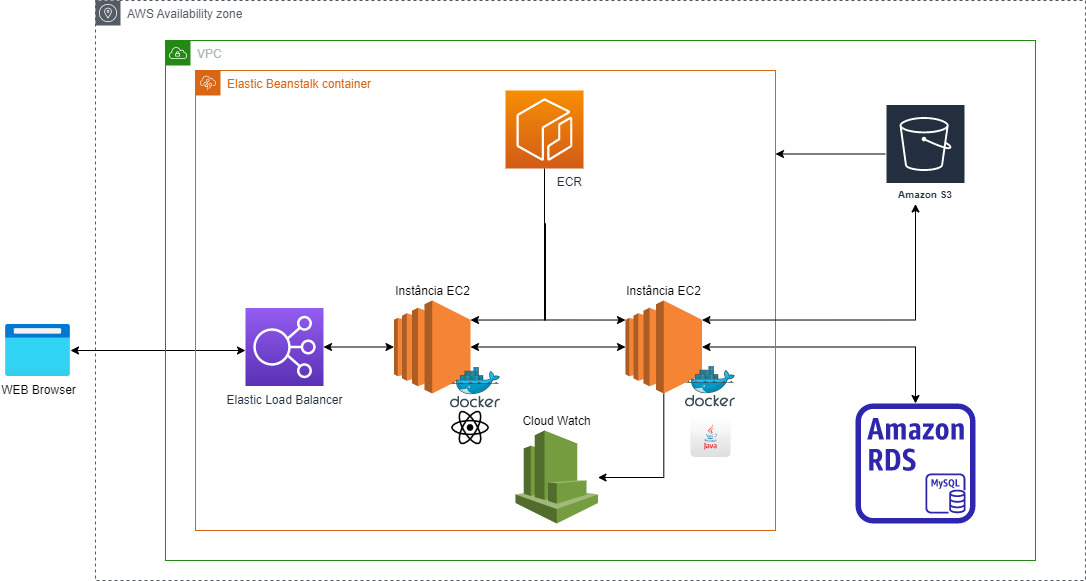
\includegraphics[width=0.9\textwidth]{ArquiteturaAplicacao.png}
        	\label{fig:infra}
        	
        	\centering
            {\footnotesize Fonte: Elaborado pelos autores.}
   \end{figure}


\section{Métricas}

    Foram geradas diferentes métricas para acompanhar o desenvolvimento do projeto, porém, devido a dificuldades enfrentadas pelos membros, as métricas não correspondem fielmente a contribuição de cada um dos envolvidos. Alguns integrantes encontraram barreiras em subir sua contribuição nos diferentes meios de controle de versionamento, como SVN e GitHub, e o trabalho foi repassado para que outro integrante fizesse o \emph{upload} do arquivo gerado.
    Tais barreiras prejudicaram a geração das métricas adequadas, e nota-se que muitos \emph{uploads} e \emph{commits} aparecem como picos após longos períodos de inatividade, porém a equipe trabalhou de forma contínua, durante as semanas que se desenvolveu o projeto. 
    
    Outro ponto de atenção é com relação ao período utilizado para gerar as métricas do GitStats, pois ele conta a partir das últimas 32 semanas, sendo que, até o momento de gerar as estatísticas, o projeto desenvolveu-se nas últimas 14 semanas.
    
    \subsection{GitStats}
    
    O Github foi o meio que a equipe encontrou de compartilhar seu progresso no projeto, por ser um serviço que todos estavam familiarizados. Apesar disso, cada integrante fazia seu upload de forma diferente, alguns fazendo o commit diretamente na interface do navegador, enquanto outros atualizavam seus commits utilizando a função pull request (principalmente na parte de desenvolver o código do sistema). Essa diferença entre formas de subir os dados na plataforma GitHub influenciou os resultados estatísticos obtidos com o GitStats. Nota-se que apesar de alguns integrantes desenvolverem muitas linhas de códigos, por serem dentro de um mesmo commit, isso reduziu a porcentagem calculada de contribuição dos integrantes em questão. 
    
    Novamente, deve-se observar que o \emph{pair programming} feito em sala de aula, onde os integrantes criavam o código juntos, porém apenas um logado no sistema e enviando as linhas produzidas, interferiu no resultado das métricas, o que omitiu a participação de todos os integrantes envolvidos.
    
    Foram geradas métricas utilizando o GitStats para 3 diferentes repositórios, que levaram em conta a divisão macro do projeto: Documentos (todos os textos feitos pelos integrantes em LaTeX, no documento compartilhado no Overleaf, assim como as propostas iniciais e apresentações), \emph{front-end} (todos os \emph{commits} de códigos referentes ao\emph{front-end} tanto da POC, como do MVP) e \emph{back-end} (todos os \emph{commits} de códigos referentes ao \emph{back-end} tanto da POC, como do MVP).
    
    
    \subsubsection{GitStats do Repositório Documentos}
    
    Neste repositório foram adicionados todo o desenvolvimento textual do projeto, assim como os slides das apresentações, propostas iniciais e foi o primeiro repositório da equipe a ser criado. 
    
    No gráfico presente na Figura \ref{fig:semanas contadas}, é possível ver que as atividades iniciam-se de acordo com o semestre corrente, contando retrospectivamente a partir da geração da métrica em 20 de Novembro de 2022, conforme observado na Figura \ref{fig:geralDoc}.
    
    \begin{figure}[H]
                \centering
                \caption{Visão Geral do Documento - GitHub.}
                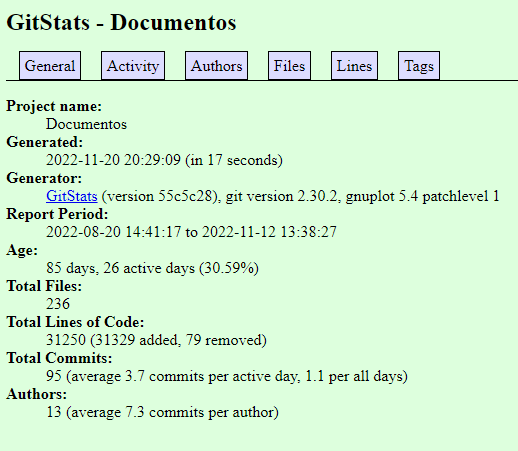
\includegraphics[width=1 \textwidth]{Gitstats/documento/geralDoc.png}
                {\footnotesize Fonte: Elaborado pelos autores.}
                \label{fig:geralDoc}
            \end{figure}
    
    
      \begin{figure}[H]
                \centering
                \caption{Gráfico das Semanas Contadas}
                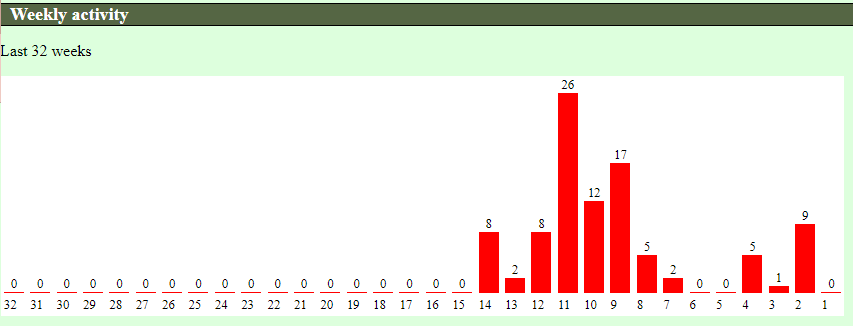
\includegraphics[width=1 \textwidth]{Gitstats/documento/semanas contadas.png}
                \label{fig:semanas contadas}
                \centering
                
            \footnotesize Fonte: Elaborado pelos autores.
            \end{figure}
    
      \begin{figure}[H]
                \centering
                \caption{Gráfico dos Dias da Semana}
                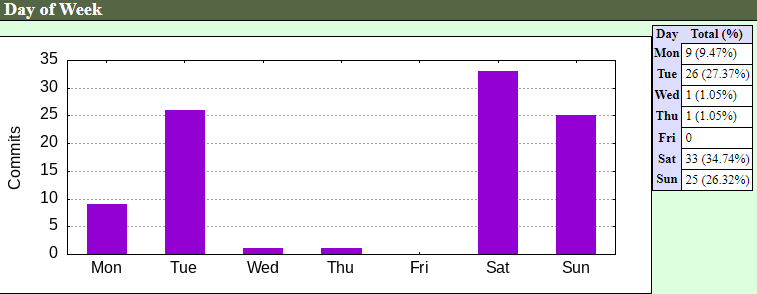
\includegraphics[width=1 \textwidth]{Gitstats/documento/dias da semana.png}
                
                \label{fig:diadasemana}
                \centering
            \footnotesize Fonte: Elaborado pelos autores.
            \end{figure}
    
    No gráfico presente na Figura \ref{fig:diadasemana} nota-se o padrão de desenvolvimento coincidindo com os dias reuniões, indo de sábado até terça. A queda nos \emph{commits} de quarta a sexta é justificada pelo fato dos integrantes cursarem outras matérias no curso, que também demandam dedicação.
    
      \begin{figure}[H]
                \centering
                \caption{Gráfico das Horas do Dia.}
                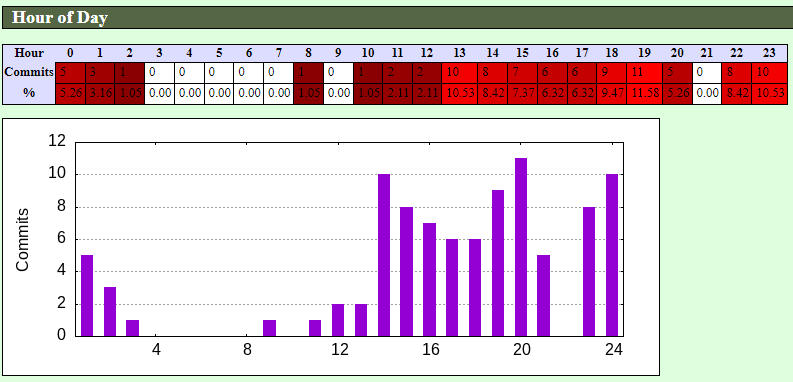
\includegraphics[width=1 \textwidth]{Gitstats/documento/horasdodia.png}
                {\footnotesize Fonte: Elaborado pelos autores.}
                \label{fig:horadodia}
            \end{figure}
            
    Com relação aos autores dos \emph{commits}, nota-se que os integrantes aparecem duplicados na Figura \ref{fig:listaautores}. Essa repetição se dá por causa da forma de envio dos dados. Na Figura \ref{fig:dominio} é possível ver os diferentes domínios utilizados pelos autores, que impactou o resultado. O gráfico de commits por autor encontra-se na Figura \ref{fig:commitautor}
    
    \begin{figure}[H]
                \centering
                \caption{Lista de Autores.}
                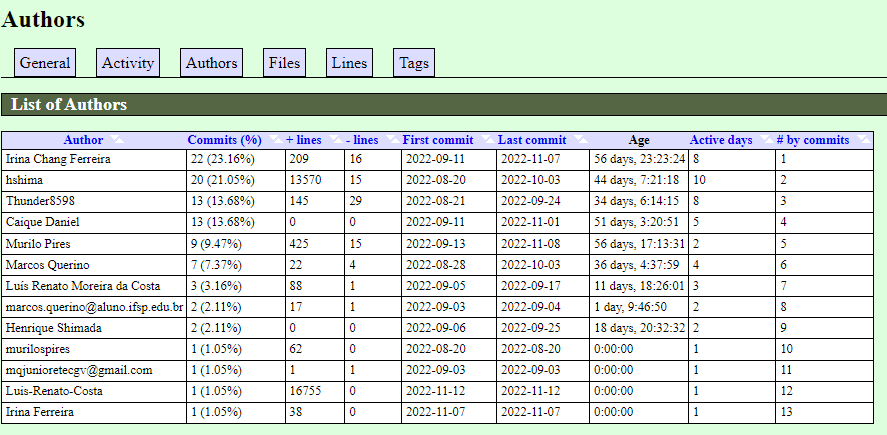
\includegraphics[width=1 \textwidth]{Gitstats/documento/lista de autores.png}
                {\footnotesize Fonte: Elaborado pelos autores.}
                \label{fig:listaautores}
            \end{figure}
            
    \begin{figure}[H]
                \centering
                \caption{Domínio Utilizado pelos Autores.}
                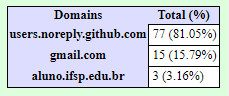
\includegraphics[scale = 1.5]{Gitstats/documento/dominios1.png}
                
                {\footnotesize Fonte: Elaborado pelos autores.}
                \label{fig:dominio}
            \end{figure} 
            
            
    \begin{figure}[H]
                \centering
                \caption{Gráfico de \emph{Commits} por Autor.}
                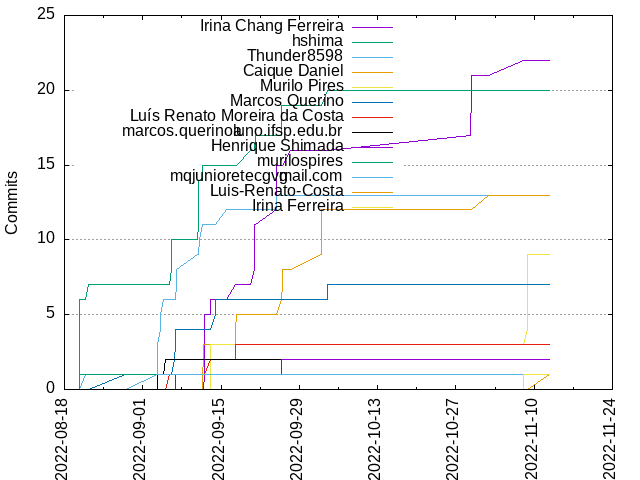
\includegraphics[width=1 \textwidth]{Gitstats/documento/commitsPorAuthor.png}
                {\footnotesize Fonte: Elaborado pelos autores.}
                \label{fig:commitautor}
            \end{figure}
            


\subsubsection{GitStats do Repositório do \emph{Front-end}}
    Nas Figuras \ref{fig:geralFront}, \ref{fig:semanasFront}, \ref{fig:diasemanaFront}, \ref{fig:horasFront}, \ref{fig:autorFront}, \ref{fig:commitFront} e \ref{fig:extensaoFront} são expostas as métricas geradas no repositório \emph{Front-end}.
    
    \begin{figure}[H]
                \centering
                \caption{Visão Geral do Front-end} - GitHub.
                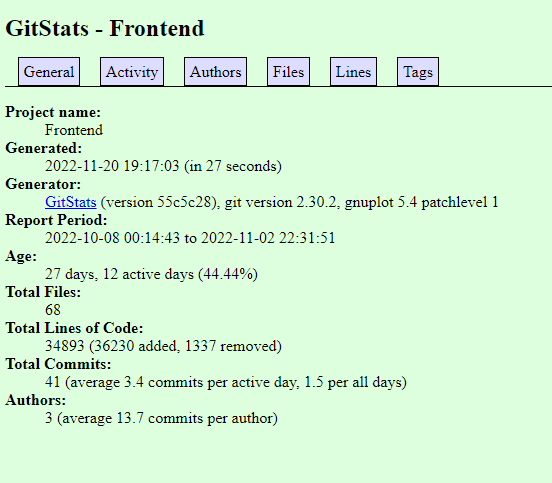
\includegraphics[width=1 \textwidth]{Gitstats/front-end/geralFront.png}
                {\footnotesize Fonte: Elaborado pelos autores.}
                \label{fig:geralFront}
            \end{figure}
    
    \begin{figure}[H]
                \centering
                \caption{Gráfico de Semanas Contadas.}
                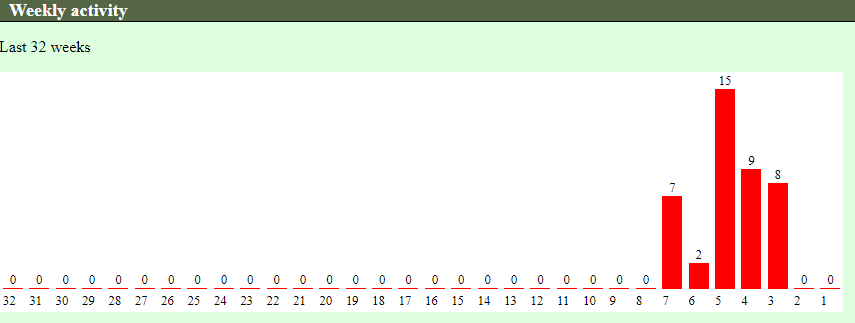
\includegraphics[width=1 \textwidth]{Gitstats/front-end/SemanasFront.png}
                {\footnotesize Fonte: Elaborado pelos autores.}
                \label{fig:semanasFront}
            \end{figure}
            
            \begin{figure}[H]
                \centering
                \caption{Gráfico de Dias da Semana do  Front-end.}
                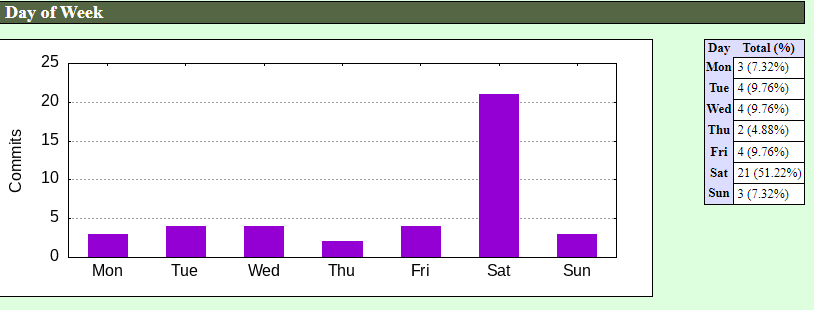
\includegraphics[width=1 \textwidth]{Gitstats/front-end/DiasdaSemana.png}
                {\footnotesize Fonte: Elaborado pelos autores.}
                \label{fig:diasemanaFront}
            \end{figure}
            
            \begin{figure}[H]
                \centering
                \caption{Gráfico de Horas por Dia do Front-end.}
                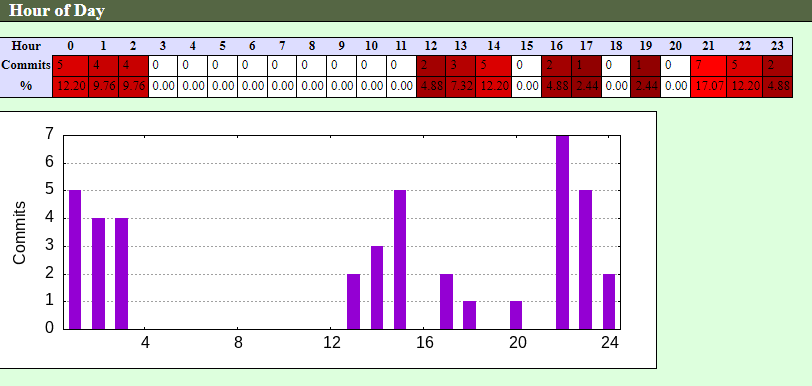
\includegraphics[width=1 \textwidth]{Gitstats/front-end/HorasdoDia.png}
                {\footnotesize Fonte: Elaborado pelos autores.}
                \label{fig:horasFront}
            \end{figure}
            
            \begin{figure}[H]
                \centering
                \caption{Lista de Autores do
                Front-end.}
                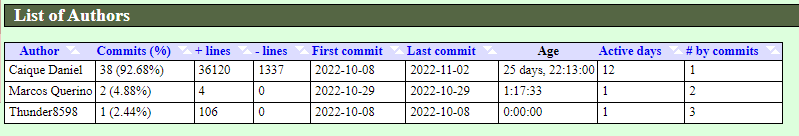
\includegraphics[width=1 \textwidth]{Gitstats/front-end/ListaAutores.png}
                {\footnotesize Fonte: Elaborado pelos autores.}
                \label{fig:autorFront}
            \end{figure}
            
            \begin{figure}[H]
                \centering
                \caption{Gráfico de Commits por Autor.}
                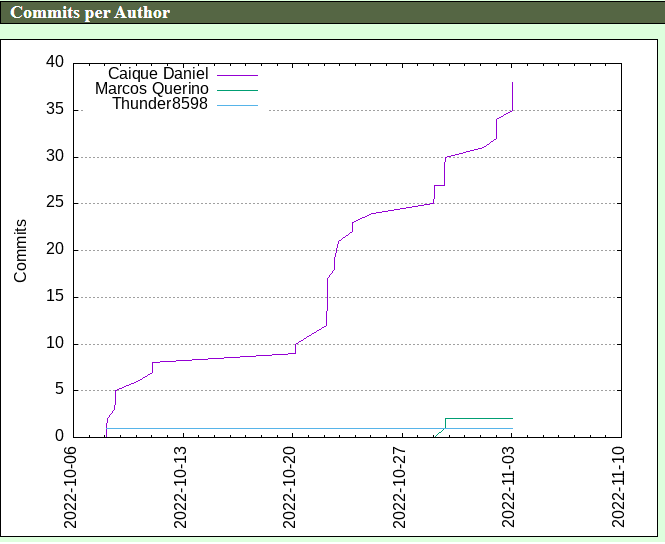
\includegraphics[width=1 \textwidth]{Gitstats/front-end/CommitsPorAutor.png}
                {\footnotesize Fonte: Elaborado pelos autores.}
                \label{fig:commitFront}
            \end{figure}
    
    \begin{figure}[H]
                \centering
                \caption{Extensões utilizadas no \emph{Front-end}.}
                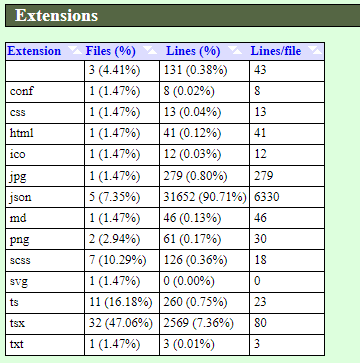
\includegraphics[scale = 1.2]{Gitstats/front-end/ListadeExtensoes.png}
                
                {\footnotesize Fonte: Elaborado pelos autores.}
                \label{fig:extensaoFront}
            \end{figure}
    
    
    
\subsubsection{GitStats do Repositório \emph{back-end}}

    Neste repositório houve alguns erros na geração de dados coerentes. Devido o repositório encontrar-se como privado, os dados não estavam sendo gerados. Após tornarmos o mesmo para público, foi possível gerar as métricas, mas elas foram contabilizadas como um único dia. Não conseguimos descobrir a causa dessa incoerência de resultados. 
    Pode-se conferir os resultados gerados na sequência de Figuras \ref{fig:geralBack}, \ref{fig:semanasBack}, \ref{fig:diasBack}, \ref{fig:HorasBack}, \ref{fig:AutorBack}, \ref{fig:commitBack} e \ref{fig:extensoesBack}.
    
    \begin{figure}[H]
                \centering
                \caption{Visão Geral do \emph{back-end} - GitHub.}
                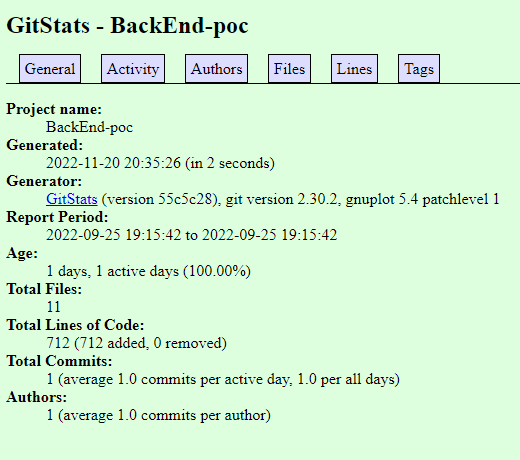
\includegraphics[width=1 \textwidth]{Gitstats/back-end/GeralBack.png}
                {\footnotesize Fonte: Elaborado pelos autores.}
                \label{fig:geralBack}
            \end{figure}
    
    
    \begin{figure}[H]
                \centering
                \caption{Gráfico de Semanas Contadas.}
                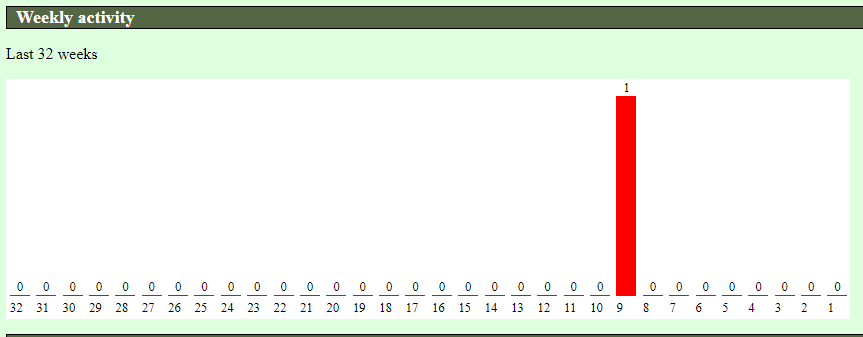
\includegraphics[width=1 \textwidth]{Gitstats/back-end/SemanasBack.png}
                {\footnotesize Fonte: Elaborado pelos autores.}
                \label{fig:semanasBack}
            \end{figure}
            
            \begin{figure}[H]
                \centering
                \caption{Gráfico de Dias da Semana do \emph{back-end}.}
                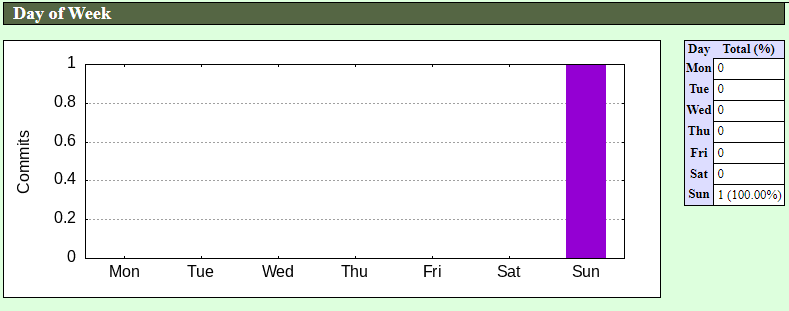
\includegraphics[width=1 \textwidth]{Gitstats/back-end/DiasBack.png}
                {\footnotesize Fonte: Elaborado pelos autores.}
                \label{fig:diasBack}
            \end{figure}
            
            \begin{figure}[H]
                \centering
                \caption{Gráfico de Horas por Dia do \emph{back-end}.}
                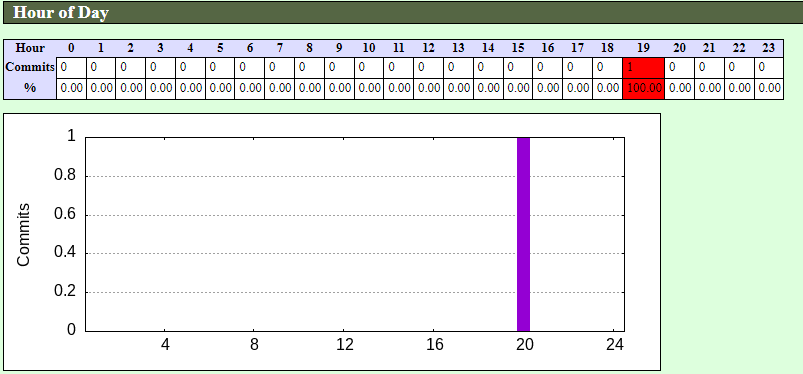
\includegraphics[width=1 \textwidth]{Gitstats/back-end/HorasBack.png}
                {\footnotesize Fonte: Elaborado pelos autores.}
                \label{fig:HorasBack}
            \end{figure}
            
            \begin{figure}[H]
                \centering
                \caption{Lista de Autores do \emph{back-end}.}
                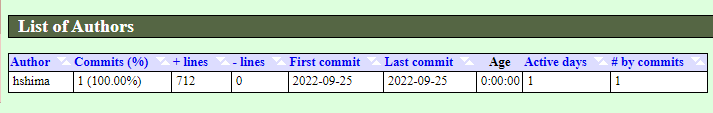
\includegraphics[width=1 \textwidth]{Gitstats/back-end/AutorBack.png}
                {\footnotesize Fonte: Elaborado pelos autores.}
                \label{fig:AutorBack}
            \end{figure}
            
            \begin{figure}[H]
                \centering
                \caption{Gráfico de Commits por Autor.}
                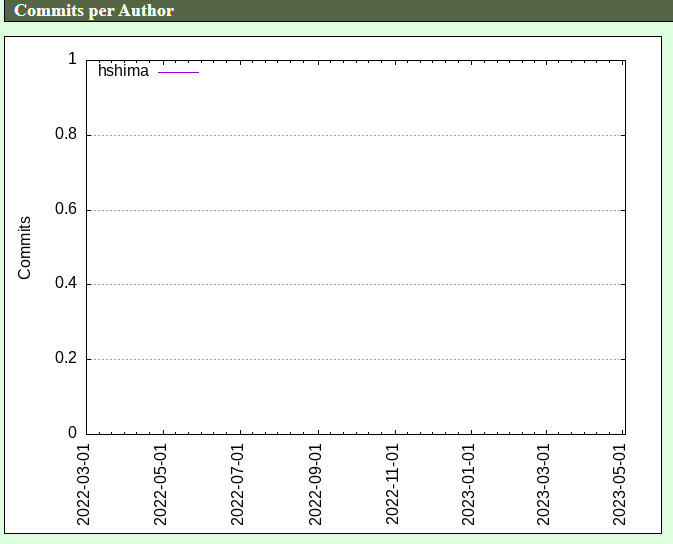
\includegraphics[width=1 \textwidth]{Gitstats/back-end/commitsAutorBack.png}
                {\footnotesize Fonte: Elaborado pelos autores.}
                \label{fig:commitBack}
            \end{figure}
            
            \begin{figure}[H]
                \centering
                \caption{Lista de Extensões Utilizadas no \emph{back-end}.}
                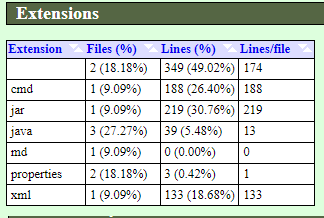
\includegraphics[scale = 1.2]{Gitstats/back-end/extensoesBack.png}
                
                {\footnotesize Fonte: Elaborado pelos autores.}
                \label{fig:extensoesBack}
            \end{figure}
    
    
\subsection{StatSVN}

    O Subversion, ou SVN foi utilizado para controlar as entregas feitas pela equipe aos professores. Ressaltamos que apenas 3 integrantes conseguiram efetivamente realizar as entregas por esse sistema, o que gerou um resultado não fidedigno da realidade, visto que todos os integrantes participaram do desenvolvimento. 
    
    Nas Figuras \ref{fig:desenvolvimentoSVN}, \ref{fig:linhaCod}, \ref{fig:diaSemana} e \ref{fig:horaDia} são expostas as métricas geradas pelo StatSVN.
    
    \begin{figure}[H]
                \centering
                \caption{Visão Geral do Desenvolvimento no SVN.}
                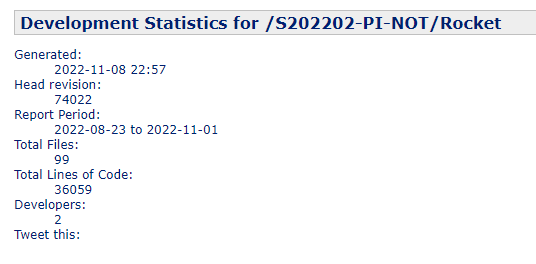
\includegraphics[width=1 \textwidth]{StatSVN/StatDesenvolvimento.png}
                {\footnotesize Fonte: Elaborado pelos autores.}
                \label{fig:desenvolvimentoSVN}
            \end{figure}
    
    \begin{figure}[H]
                \centering
                \caption{Gráfico Referentes as Linhas de Códigos.}
                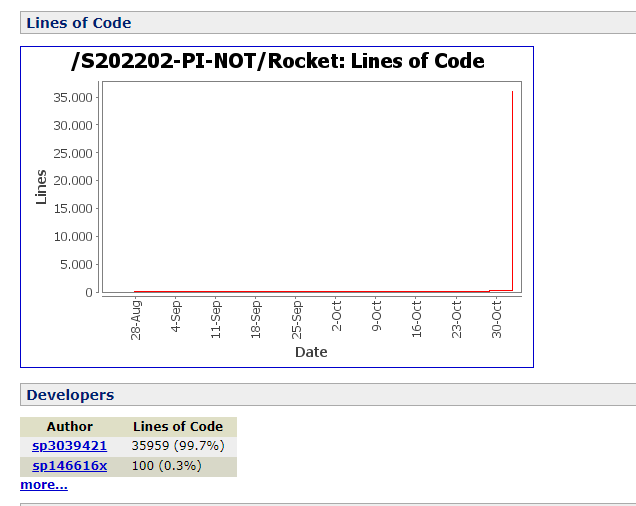
\includegraphics[width=1 \textwidth]{StatSVN/linha de codigo autor.png}
                {\footnotesize Fonte: Elaborado pelos autores.}
                \label{fig:linhaCod}
            \end{figure}
    
    \begin{figure}[H]
                \centering
                \caption{Gráfico Referente aos Dia da Semana.}
                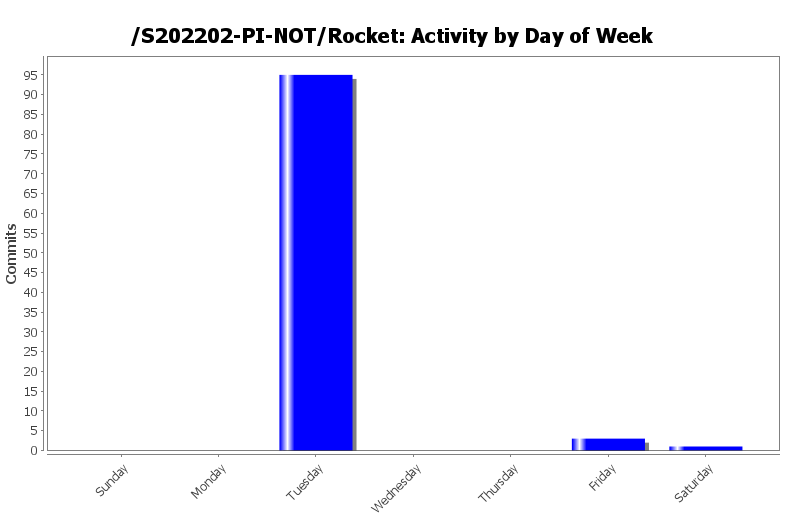
\includegraphics[width=1 \textwidth]{StatSVN/DiadaSemana.png}
                {\footnotesize Fonte: Elaborado pelos autores.}
                \label{fig:diaSemana}
            \end{figure}
    
    \begin{figure}[H]
                \centering
                \caption{Gráfico Referentes as Horas do Dia.}
                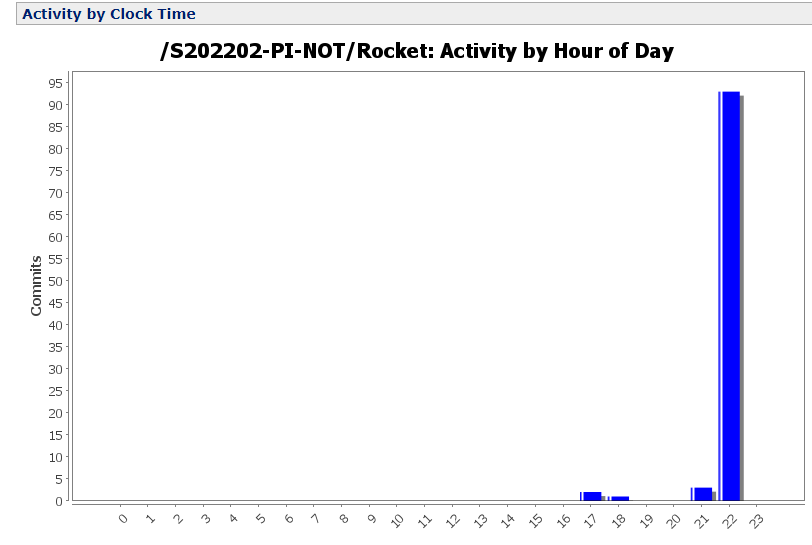
\includegraphics[width=1 \textwidth]{StatSVN/HoradoDia.png}
                {\footnotesize Fonte: Elaborado pelos autores.}
                \label{fig:horaDia}
            \end{figure}

\section{Testes de Segurança}

\subsection{Teste de Segurança dos Headers}

\begin{figure}[H]
    \centering
    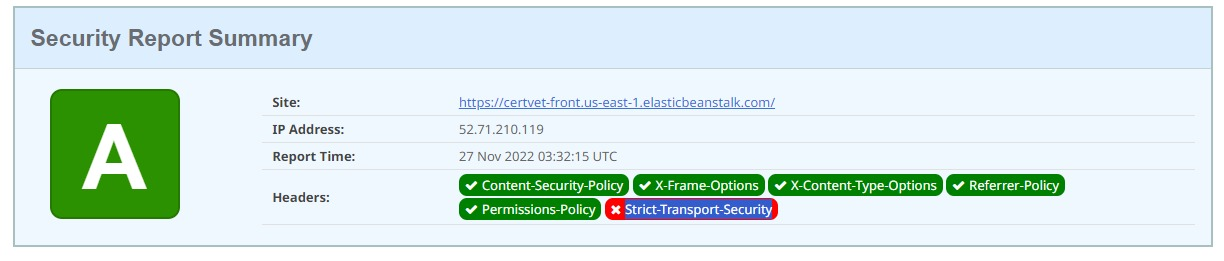
\includegraphics[width=1 \textwidth]{images/headers1.jpeg}    \caption{Resultado do Teste de Headers}
    \label{fig:header}
\end{figure}

\subsection{Teste de Segurança SSL}
    Além da implementação do TLS, foram adicionadas políticas de segurança através dos Headers das requisições, de forma a instruir o navegador sobre as ações que são permitidas no site.
    Como referência para a verificação de Headers de segurança, foi orientada a utilização do site Security Headers\citeonline{header}.
    Para a configuração dos Headers, foi utilizado como referência os site MDN Web Docs \citeonline{mdn}.

    
\subsubsection{ Teste de Segurança Inicial}

    Antes de realizar qualquer tentativa de implementação, foi realizado um teste com a aplicação no estado atual (as is). Posteriormente, para documentar a situação, foi realizada uma nova consulta adicionada ao apêndice, onde obteve-se o seguinte resultado mostrado na Figura \ref{fig:sslFront}

    \begin{figure}[H]
        \centering
        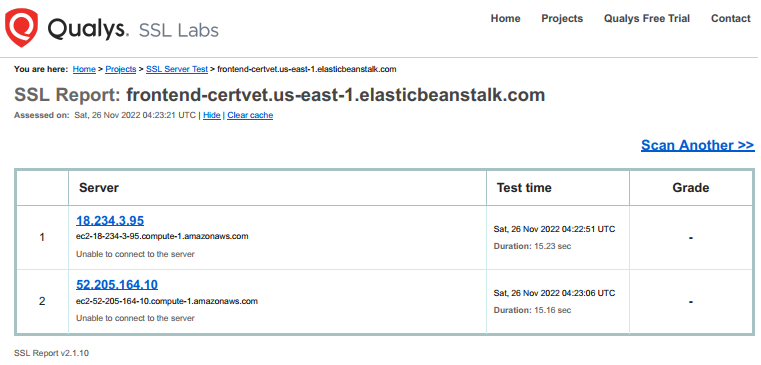
\includegraphics[width=0.9 \textwidth]{images/headerfront.png}
        \caption{Teste SSL da Aplicação}
        \label{fig:sslFront}
    \end{figure}
    
\subsubsection{Teste de Segurança Final}

Após alguns ajustes e mais estudos sobre os certificados de segurança, obteve-se o seguinte resultado mostrado na Figura \ref{fig:sslFrontfinal} e também no Apêndice \ref{apendiceE}

\begin{figure}[H]
        \centering
        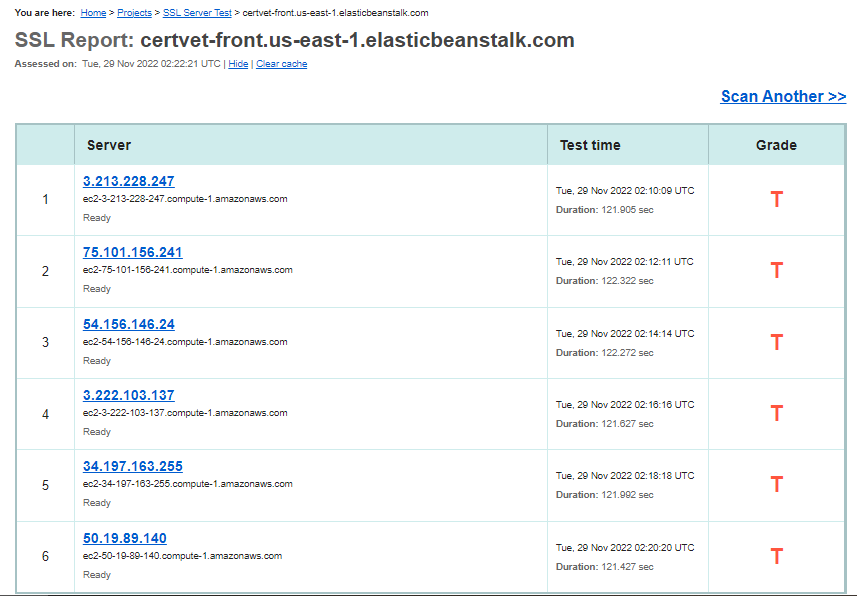
\includegraphics[width=0.9 \textwidth]{images/sslFront.png}
        \caption{Teste SSL da Aplicação Final}
        \label{fig:sslFrontfinal}
    \end{figure}
    
%%%%%%%%% TODO ajustar texto de considerações finais %%%%%%%%%%%%%%%%%%%%%%

\chapter[Conclusão]{Conclusão}

    A acessibilidade de tecnologias em nuvem e emprego de tecnologias portáveis de containerização permitem que aplicações sejam criadas e transportadas com mínimo de interferência para o mantenedor e seus clientes. Entretanto, ao utilizar soluções proprietárias, como o serviço Amazon S3, é necessário considerar o tipo de comprometimento por vendor lock in que corre-se o risco de expor a aplicação.

    Em suma, as utilização e aproveitamento de recursos computacionais, principalmente em nuvem, na área de medicina veterinária faz-se não somente benéfica por eliminar o risco de perda de dados em mídias físicas e aumentar a velocidade de recuperação de dados importantes e sensíveis.

    As normas que regulam as atividades médico-veterinárias, em especial sobre medicação controlada, podem sofrer alterações que nem sempre são acompanhadas pelo técnico no momento em que são publicadas. Uma ferramenta de gestão focada nesta atividade reduz o risco do negócio se enquadrar em uma situação de irregularidade.

    \chapter[Links do Projeto]{Links do Projeto}
    % no momento este tópico fica como capitulo, mas na entrega final ele vai virar um tópico do capitulo de métricas
    \begin{figure} [htb!]
        \centering
        
\includegraphics[width=0.3\textwidth]{qrcode/qrcode_GIT.png}
        \caption{Link Repositório no GitHub}
        {\footnotesize \url{ https://github.com/orgs/EquipeRocketIFSP/repositories}}
        \label{fig:qrcode_GIT}
    \end{figure}

    \begin{figure}[htb!]
        \centering
        
\includegraphics [width=0.3\textwidth]{qrcode/qrcode_YT.png}
        \caption{Link Página no YouTube}
        {\footnotesize \url{https://youtube.com/@equiperocket6085}}
        \label{fig:qrcode_YT}
    \end{figure}
    
    \begin{figure}[htb!]
        \centering
        
\includegraphics[width=0.3\textwidth]{qrcode/qrcode_BLOG.png}
        \caption{Link Página do Blog}
        {\footnotesize \url{https://equipe-rocket-ifsp.blogspot.com}}
        \label{fig:qrcode_BLOG}
    \end{figure}
    
    \begin{figure}[htb!]
        \centering
        
\includegraphics[width=0.3\textwidth]{qrcode/svn.png}
        \caption{Link Repositório da Equipe no SVN}
        {\footnotesize \url{https://svn.spo.ifsp.edu.br/svn/a6pgp/S202202-PI-NOT/Rocket}}
        \label{fig:svn}
    \end{figure}
    
   
    \begin{figure}[htb!]
         \centering
         \includegraphics[width=0.3\textwidth]{qrcode/qrcode_SITE.png}
         \caption{\emph{Site} CertVet}
         {\footnotesize \url{https://certvet-front.us-east-1.elasticbeanstalk.com}}
         \label{fig:linksite}
         \end{figure}

    
    \chapter[Considerações Finais]{Considerações Finais}

    A equipe encontrou diversas dificuldades ao longo do projeto, que serviram de aprendizado para a carreira na área da Tecnologia da Informação.
    A organização e distribuição das tarefas provou-se ser a habilidade mais valiosa que uma equipe deve ter, não diminuindo a capacidade intelectual de cada um dos membros. 
    
    Fatores externos também impediram que a equipe pudesse entregar o projeto idealizado nas primeiras reuniões do curso. O principal impedimento foi a recusa do orgão fiscalizador federal, CFMV, de liberar acesso á sua API, acesso que, caso fosse concedido, permitiria validar o registro do profissional que acessa o sistema, garantindo uma segurança à aplicação e àqueles que a usam. O contato, via Lei de Acesso a informação foi feito em dois emails, que podem ser vistos no Apêndice \ref{apendiceA}  e \ref{apendiceC}. Assim como a resposta do CFMV dada ao primeiro contato, vista no Apêndice \ref{apendiceB}.
    
    Outro fator externo se deu com relação aos testes de segurança, visto que o serviço de servidor escolhido através da AWS não estava configurado para atender todos os requisitos necessário para atingir a nota mínima exigida pelos professores. Com isso mudamos a entrega desse requisito para a entrega final do documento.
    

%---
% pós-textual
% ---


\postextual

% quando não esta utilizando biblatex tem que carregar as referencias aqui
\IfPackageLoaded{biblatex}{%
\printbibliography

\ifthenelse{\boolean{utilizarREFINDENT}}{%
}

}{%
\bibliography{referencias,exemplos/abntex2-doc-abnt-6023}
}

%% ----------------------------------------------------------
% Glossário
% ----------------------------------------------------------
%
%
\ifdef{\printnoidxglossary}{
    \addcontentsline{toc}{chapter}{GLOSSÁRIO}
    \printnoidxglossary[style=glossario]
    %\printglossaries
}{}

% ----------------------------------------------------------
% Apêndices
% Documentos gerados pelo próprio autor
% ----------------------------------------------------------

% ---
% Inicia os apêndices
% ---
\begin{apendicesenv}

% Imprime uma página indicando o início dos apêndices
\partapendices

% ----------------------------------------------------------
%\chapter{Quisque libero justo}
% ----------------------------------------------------------

%\preencheComTexto

\begin {appendices}
\chapter{Email de Contato Inicial}



\includegraphics[page=1, width=1\linewidth,height=0.8\textheight]{Apêndices/email1.PNG}

\newpage
\label{apendiceA}
\end{appendices}

\begin {appendices}
\chapter{Email de Resposta CFMV}
\includegraphics[page=1, width=1\linewidth,height=0.8\textheight]{Apêndices/emailresposta.png}

\newpage
\label{apendiceB}
\end{appendices}
\newpage

\begin {appendices}
\chapter{Novo Contato ao CFMV}


\includegraphics[page=1, width=1\linewidth,height=0.8\textheight]{Apêndices/email2.png}

\label{apendiceC}
\end{appendices}

\begin {appendices}
\chapter{Teste de Headers}
\includegraphics[page=1, width=1\linewidth,height=0.8\textheight]{Apêndices/headersfinal.pdf}
\label{apendiceD}
\end{appendices}

\begin {appendices}
\chapter{Teste de SSL}
\includegraphics[page=1, width=1\linewidth,height=0.8\textheight]{Apêndices/sslFront.pdf}
\label{apendiceE}
\end{appendices}

\begin {appendices}
\chapter{Blog da Equipe}
\includegraphics[page=1, width=1\linewidth,height=0.8\textheight]{Apêndices/EquipeRocketBlog.pdf}

\includepdf[pages={2-},scale=0.80,pagecommand={}]{Apêndices/EquipeRocketBlog.pdf}

\end{appendices}








%\newpage
%\chapter{Email de Contato Inicial}
%\begin{figure}
  %%   \includegraphics[width=1\textwidth]{Apêndices/email1.PNG}
 %  \caption{Email de contato inicial.}
 %   \label{email1}
%\end{figure}





%\chapter{Email de Resposta do CFMV}
%\begin{figure}
 %   \centering
  %  \includegraphics[width=1\textwidth]{Apêndices%/emailresposta.png}
   % \caption{Resposta enviada pelo CFMV}
    %\label{resposta}
%\end{figure}



%\chapter{Novo Contato ao CFMV}

%\begin{figure}
 %   \centering
  %  \includegraphics[width=1\textwidth]{Apêndices/email2.png}
   % \caption{Email de contato com as leis}
%    \label{email2}
%\end{figure}
% ----------------------------------------------------------
%\chapter{Nullam elementum urna vel imperdiet sodales elit ipsum pharetra ligula
%ac pretium ante justo a nulla curabitur tristique arcu eu metus}
% ----------------------------------------------------------
%\preencheComTexto
\
%\begin{figure}
  %  \centering
  %  \includegraphics{Apêndices/EquipeRocketBlog.pdf}
   % \caption{Caption}
    %\label{fig:my_label}
%\end{figure}

\end{apendicesenv}
% ---




% ----------------------------------------------------------
% Anexos
% Documentos gerados por outros autores
% ----------------------------------------------------------

% ---
% Inicia os anexos
% ---
\begin{anexosenv}
\anexos
% Imprime uma página indicando o início dos anexos
\partanexos

% ---
\chapter{Manual todonotes(parcial)}
\label{manual-todonotes}
% ---
\index{pdf}
% se pages = "-"  fica com arquivo completo
\includepdf[pages=1-3,scale=0.8,frame=true,pagecommand={}]{anexos/todonotes.pdf}

% ---
% Para incluir sem gerar a quebra de página inicial no anexo
\includepdf[pages=1,scale=0.7,frame=true,pagecommand=\chapter{Manual pdfpages(parcial)}\label{manual-pdfpages}]{anexos/pdfpages.pdf}
\includepdf[pages=2-3,scale=0.8,frame=true,pagecommand={}]{anexos/pdfpages.pdf}

% ---
\chapter{Manual acronym(parcial)}
\index{pdf}
% somente algumas páginas para exemplo sem borda
\includepdf[pages=1-3,frame=false,pagecommand={}]{anexos/acronym.pdf}



\includepdf[frame=true,scale=0.7,pagecommand=\chapter{Referência Rápida pifont}\label{pifont-quickref}]{anexos/pifont.pdf}


\end{anexosenv}





\end{document}


%
% ----------------------------------------------------------
% Introdução
% ----------------------------------------------------------

\chapter[Introdução]{Introdução}
    Os estabelecimentos veterinários estão sujeitos a rigorosas leis e fiscalização por parte dos órgãos de classe (\acs{crmvs} e \acs{cfmv}). São exigidos documentos comprobatórios dos atendimentos, procedimentos e medicações utilizadas, que devem ser guardados por um prazo de 2 a 20 anos. Tais documentos são usados tanto para fins de fiscalização, como para fins jurídicos, em caso de processos, assim como devem estar disponíveis para o tutor do animal.
    
    Prontuários veterinários em formato digital são oferecidos por diversos sistemas de gerenciamento de clínicas veterinárias, e são amplamente usados como forma de garantir um backup dos prontuários de forma simples, segura e efetiva.
    Apesar disso, as versões digitais não podem ser utilizadas como documentos oficiais em caso de provas judiciais. 
    
    A gestão de medicamentos controlados (de uso restrito e com retenção de receitas, de acordo com as leis vigentes da INSTRUÇÃO NORMATIVA Nº 35, DE 11 DE SETEMBRO DE 2017, Capítulo I, art 2º, § IV, Capitulo IV, § 11  \cite{normativa} é feita utilizando um caderno, de capa dura, no formato brochura, onde o médico veterinário responsável técnico (RT) anota as datas de entrada dos medicamentos no estoque e quanto desse medicamento foi utilizado no dia, para cada procedimento. Este caderno é denominado Livro-Registro.


\section{Análise da situação atual}
    
\section{Problema}
    Assumindo as seguintes premissas:

    \begin{itemize}
        \item 
        Os sistemas de prontuários digitais existentes no mercado permitem a edição e alteração dos dados inseridos, sem garantir um histórico dessas alterações, ou meios de rastrear as alterações, em caso de fiscalização por órgão públicos ou perícias judiciais.
        
        \item
        Os arquivos são armazenados de forma física (utilizando pastas-fichários) e são carimbados e assinados pelo médico veterinário.
        
        \item
        O gerenciamento dos medicamentos controlados feitos em livro-registro demandam um tempo extra, gasto pelo profissional, que deve fazer as contas manualmente para cada valor, muitas vezes tendo que anotar em diversos documentos os mesmos dados.
        
        \item
        O armazenamento desses arquivos ocupa espaço e estão sujeitos a danos e perdas por mau armazenamento (umidade, fogo, roubo, etc).
        
        \item
        O preenchimento desses dados em versões físicas e depois transpostos para versões digitais é demorado e sujeito a falhas, demandando um tempo que poderia ser melhor empregado para os envolvidos.
        
        \item
        A consulta a esses documentos pode ser prejudicada caso não haja uma boa organização por parte dos responsáveis pelo estabelecimento.
    \end{itemize}


    Partindo dos fatos relacionados, como armazenar informações de dados documentais virtuais em clínicas veterinárias que possam ser aceitas como documentos oficiais pelo órgão de classe?

\section{Objetivos}
    \explicacao{Em muitos casos uma seção única de objetivos é suficiente}
    \preencheComTexto
    
    \subsection{Objetivo Principal}
    \preencheComTexto
    
    \subsection{Objetivos Secundários}
    \preencheComTexto
    
    \section{Justificativa}
    \preencheComTexto
    
    \section{Estrutura do Estudo}
    \preencheComTexto


%% ---
% Capitulo de revisão de literatura
% ---
\chapter{Revisão da Literatura}

\explicacao{Todos trabalhos devem possuir a revisão de literatura onde são abordados os estudos feitos com base da literatura (livros, artigos acadêmicos, publicações em periódicos), todos elementos devem ser referenciados por citações.}

\explicacao{Diversas referencias utilizadas nesse modelo não deveriam ser utilizadas diretamente em um trabalho acadêmico, mas estão aqui para demonstrar de forma mais clara alguns pontos importantes sobre desenvolvimento de projetos.}

\explicacao{Cada parágrafo da revisão de literatura deve apresentar uma ideia com base em uma referencia.}

\explicacao{Copiar e colar é plágio. Exceto em casos muito específicos onde utilizamos a citação direta você deve escrever com suas palavras (seu entendimento, parafrasear) o que os autores escreveram na publicação original.}

\explicacao{Não são abordados aqui itens técnicos que normalmente são vistos em disciplinas anteriores do curso (UML, banco de dados, metodologias de gerenciamento de projeto etc...), esses elementos podem receber citações nos outros capítulos do trabalho. Essa regra não se aplica aos trabalhos de pós graduação quando o tema estiver relacionado a conceitos técnicos.}


\preencheComTexto
% ---

% ---
\section{Assunto 1}
\preencheComTexto

\section{Assunto 2}
\preencheComTexto

\section{Assunto 3}
\preencheComTexto

\section{Assunto X}
\preencheComTexto
% ---


% Para facilitar a manutenção é sempre melhore criar um arquivo por capitulo, para exemplo isso não é necessário 
%% Para facilitar a manutenção é sempre melhore criar um arquivo por capitulo, para exemplo isso não é necessário 

%---------------------------------------------------------------------------------------
\chapter{Modelo Teórico e Pressupostos (ou Hipóteses) da Pesquisa}
\explicacao{Para trabalho da Pós Graduação}
\preencheComTexto




%---------------------------------------------------------------------------------------
\chapter{Métodos de Pesquisa}
\explicacao{Para trabalho da Pós Graduação}
\preencheComTexto

\section{Tipo de Pesquisa}
\preencheComTexto

\section{Plano Amostral (se Pesquisa Quantitativa)}
\preencheComTexto

\section{Instrumento de Pesquisa e Escalas Utilizadas (Escalas se Pesquisa Quantitativa)}
\preencheComTexto

\section{Coleta de Dados}
\preencheComTexto

\section{Análise de Dados}
\preencheComTexto


%---------------------------------------------------------------------------------------
\chapter{Resultados da Pesquisa}
\explicacao{Para trabalho da Pós Graduação}
\preencheComTexto

\section{Assunto 1}
\preencheComTexto

\section{Assunto 2}
\preencheComTexto

\section{Assunto 3}
\preencheComTexto

\section{Discussão dos Resultados Observados}
\preencheComTexto

%---------------------------------------------------------------------------------------







% exemplos de escrita LaTeX e erros comuns
%\chapter{Exemplos \LaTeX}
\label{cap-exemplos}

\explicacao{ATENÇÃO : Este capítulo e os seguintes demonstram como fazer no {\LaTeX} portanto devem ser lidos em conjunto com o código fonte desse documento}

% exemplo de como inserir uma referencia adicional no sumario (normalmente não utilizado em um trabalho acadêmico)
\addcontentsline{toc}{chapter}{Exemplos que devem ser lidos (mas esse tipo de indicação não vai em um trabalho acadêmico) :-)}

Esse capítulo tem exemplos de escrita utilizando o {\LaTeX}  utilizando \abnTeX, é muito simples escrever em \textbf{negrito}, \textit{itálico} \footnote{apesar de que nesse documento \mostraComandoLaTeX{textit} \mostraComandoLaTeX{emph} tem comportamento parecido é recomendável utilizar \mostraComandoLaTeX{textit} de forma genérica para itálico}, ....


Existem diversos tutoriais para uso de \LaTeX, se você está utilizando esse modelo não precisará se preocupar com muitos dos detalhes técnicos do \LaTeX \space e cuidar somente do seu texto.

Escolha seu editor : \url{https://en.wikipedia.org/wiki/Comparison\_of\_TeX\_editors}, apesar do overleaf sem bem prático, nem todas as funções estão disponíveis na versão gratuita e você pode instalar gratuitamente em seu computador um compilador \LaTeX \space e utilizar um sistema de controle de versão para gerenciar seu documento.


\section{Normas ABNT}

Esse documento modelo já resolve boa parte da padronização NBR 14.724:2011 \cite{NBR14724:2011} que deve ser seguida e inclusive alguns pontos que não são claros pelo modelo de padronização do \ac{ifsp}.

Leia os documentos do {\abnTeX} e do \ac{ifsp}:
\begin{itemize}
    \item \url{https://www.abntex.net.br/}
    
    \item \acs{faq} : \url{https://github.com/abntex/abntex2/wiki/FAQ}
    
    \item \url{http://mirror.unl.edu/ctan/macros/latex/contrib/abntex2/doc/abntex2.pdf}
    
    \item \waUrl{https://spo.ifsp.edu.br/biblioteca?id=184}
\end{itemize}

No \ac{ifsp} você pode acessar todas as normas \ac{abnt} sem custo, as informações estão disponíveis no endereço \waUrl{https://www.ifsp.edu.br/index.php/outras-noticias/52-reitoria/2329-alunos-e-servidores-do-ifsp-podem-acessar-abnt-via-web.html}.

Apesar de alguns elementos serem opcionais na \ac{abnt} eles foram definidos como obrigatórios (folha de rosto, resumo, lista de siglas, lista de ilustrações, glossário etc), nos trabalhos completos de projetos de informática do \ac{ifsp} campus São Paulo. Documentos menores como propostas de projeto, documento de \ac{poc} não necessitam desses elementos, mas alguns podem ser uteis para ajudar no estudo do {\LaTeX} em preparação para o documento final.

\begin{itemize}
    \item Logotipo da instituição, não é citado na \ac{abnt} nem no manual de normalização do \ac{ifsp}, mas aparece em uma imagem do documento de normalização, foi definido que não deve ser incluído na capa;
    
    \item Nome da instituição que é opcional na capa, deve ser utilizado;
    
\end{itemize}



\section{Detalhes textuais}

O documento é dividido em capítulos, e cada capítulo dividido em seções utilizando o \abnTeX \space você pode dividir seus documentos nos níveis de acordo com os comandos:

\begin{itemize}
    \item \mostraComandoLaTeX{chapter}  (1);
    
    \item \mostraComandoLaTeX{section} (1.1);
    
    \item \mostraComandoLaTeX{subsection} (1.1.1);
    
    \item \mostraComandoLaTeX{subsubsection} (1.1.1.1);
    
    \item \mostraComandoLaTeX{subsubsubsection} (1.1.1.1.1).
    
\end{itemize}

Tenha em mente que normalmente se utiliza no máximo o nível \mostraComandoLaTeX{subsection}.
Ao definir as divisões do seu trabalho utilizando as diretivas do \LaTeX, elas são automaticamente inseridas no sumário do documento.


\subsection{Caracteres Reservados e auxiliares}



Alguns caracteres são reservados no \LaTeX \space e por isso para utilizar esses caracteres é necessário utilizar uma forma diferenciada de escrita. É possível utilizar a macro \mostraComandoLaTeX{symbol} com o código \ac{ascii} do caracter desejado, veja no código fonte desse texto como utilizar corretamente esses itens.


\begin{itemize}
\item barra invertida : \textbackslash   \symbol{92}    $\backslash$;
\item til  :  \symbol{126} ;
\item cifrão : \$;
\item sublinhado, \textit{underscore}, \textit{underline} : \_;
\item \enquote{aspas} as macros \mostraComandoLaTeX{enquote} / \mostraComandoLaTeX{textquote} garantem o espaçamento correto, se utilizar diretamente as ASPAS o espaçamento é perdido;
% https://tex.stackexchange.com/questions/80395/no-space-after-closing-double-quote
\item marcadores : \cmark\ \xmark\ \circlemark\ \ding{100} \ - ver mais no \refanexo{pifont-quickref};
\item chaves : \} \{.
\end{itemize}

\subsection{Listas}

Em uma lista de itens cada item deve ser terminado por ponto e virgula, exceto o ultimo item que deve ter um ponto final.

\begin{itemize}
\item item 1;
\item item 2;
\item item ..;
\item item final.
\end{itemize}


\subsection{Citações / Referências}
\label{referencias}

Em um trabalho acadêmico você deve buscar referencias que servem de base para seus estudos, essas referencias devem ser confiáveis, normalmente artigos e livros são confiáveis pois passam por um processo de revisão por especialistas na área. É importante buscar as referencias primárias e não utilizar a informação escrita por outra pessoa (referencia secundária). As citações são definidas pela \citetitle{NBR10520:2002} e as referencias pela \citetitle{NBR6023:2018}, sendo interessante observar que a \citeonline{NBR6023:2018_alteracoes} fez uma resumo com algumas das mudanças ocorridas em 2018.


A \ac{abnt} define a citação da citação (\textit{apud}), mas sua utilização não deve ser feita exceto em casos onde o documento original não possa ser acessado de nenhuma forma. Atualmente a maioria dos documentos se encontra disponível de forma digital o que permite a busca das informações em suas fontes primárias de forma que o \textit{apud} não é bem visto. 

Não é indicada a utilização de sites como Wikipedia como fonte de informações pois a Wikipedia é uma referencia secundária, já que exige que seus artigos tenham referencias da informação, e com isso a utilização da Wikipedia cai no mesmo caso da utilização de \textit{apud} indicada anteriormente, já que é possível buscar a informação diretamente na fonte primária.

Quando for necessário citar sites deve ser utilizada a ferramenta \url{https://web.archive.org}, caso não exista uma referencia salva anteriormente basta salvar e utilizar. O uso dessa ferramenta muitas vezes ajuda também a determinar a data estimada de publicação de informação quando o site já foi salvo anteriormente e não possui data de publicação disponível.



Existem diversas formas de citação que devem ser escolhidas de acordo com o contexto do texto onde são utilizadas, observe os exemplos :

\begin{itemize}
    \item \mostraComandoLaTeX{cite} - utilizada normalmente em final de paragrafo: \newline
    \cite{UML:JACOBSON} | \cite{POWELL:2006} \\ 
        \cite{SCRUMGUIDE:2013} | \cite{urani1994} |\\
        \cite{ETAL5} | \cite{ETAL4}; 
    
    \explicacao{Se as duas ultimas referencias aparecem somente com um autor, você está compilando o documento com uma versão antiga do \mostraPacoteLaTeX{abntexcite}, o overleaf em 2021-07-06 estava desatualizado}
    \explicacao{ABNT 6023:2018 8.1.1.2 recomenda para utilizar TODOS autores sempre, mas permite utilizar et al, dependendo da versão do \mostraPacoteLaTeX{abntexcite} isso não está acontecendo corretamente}

    \item \mostraComandoLaTeX{citeonline}  - utilizada normalmente em textos como \enquote{(segundo|de acordo| com) ...}: \newline
    \citeonline{UML:JACOBSON} | \citeonline{POWELL:2006} \\
        \citeonline{SCRUMGUIDE:2013} | \citeonline{urani1994} \\
        \citeonline{ETAL5} | \citeonline{ETAL4};

    \item \mostraComandoLaTeX{citeauthoronline} - raramente utilizado, quando se deseja citar somente o autor (não está implementado no \textbf{biblatex}): \newline
    \citeauthoronline{UML:JACOBSON}| \citeauthoronline{POWELL:2006} \\
        \citeauthoronline{SCRUMGUIDE:2013} | \citeauthoronline{urani1994} \\
        \citeauthoronline{ETAL5} | \citeauthoronline{ETAL4};

    \item \mostraComandoLaTeX{citeauthor} - muito pouco utilizado: \newline \citeauthor{UML:JACOBSON}| \citeauthor{POWELL:2006} \\
        \citeauthor{SCRUMGUIDE:2013}| \citeauthor{urani1994} \\
        \citeauthor{ETAL5} | \citeauthor{ETAL4};
    
    \explicacao{Se as duas ultimas referencias aparecem somente com um autor, você está compilando o documento com uma versão antiga do \mostraPacoteLaTeX{abntexcite}, o overleaf em 2021-07-06 estava desatualizado}

    \item \mostraComandoLaTeX{citetitle} - muito pouco utilizado: \newline
    \citetitle{UML:JACOBSON}|\citetitle{POWELL:2006} \\
        \citetitle{SCRUMGUIDE:2013}| \citetitle{urani1994} 
        
    \explicacao{O comando \mostraComandoLaTeX{citetitle} está disponível utilizando a biblioteca \mostraPacoteLaTeX{biblatex}}

\end{itemize}

A documentação do abntex2cite possui muitos exemplos de como utilizar corretamente cada formato de citação : \url{https://mirrors.ibiblio.org/CTAN/macros/latex/contrib/abntex2/doc/abntex2cite-alf.pdf}.

Cada formato de citação deve ser utilizado em um contexto especifico :
\begin{itemize}
    \item De acordo com \citeonline{SCRUMGUIDE:2013} .....;
    
    \item Fonte: \citeonline{SCRUMGUIDE:2013};
    
    \item sua explicação de um assunto baseado em uma referência \cite{SCRUMGUIDE:2013}.
    
\end{itemize}

ATENÇÃO : Alguns parâmetros de formatação foram alterados em 2018, mas não foram corrigidos ainda nos pacotes do \ac{abntex}, devem ser alterados manualmente ou utilizar as versões de desenvolvimento
\begin{itemize}
    \item \url{https://github.com/abntex/abntex2/issues/210}
    
    \item \url{https://github.com/abntex/biblatex-abnt/issues/42}
\end{itemize}

Os dados devem ser definidos corretamente nos arquivos \textquote{.bib} para a correta formatação no texto e na lista de referências.

Para autor com diversas publicações no mesmo ano : são geradas letras automaticamente pelo compilador de acordo com a ordem que são apresentadas na bibliografia, a letra não aparece na lista de referencias. \footnote{\url{https://github.com/abntex/biblatex-abnt/issues/20}}




\subsection{Abreviaturas / Siglas / Glossário}
\label{siglas-glossario}

Palavras que devem ser apresentadas no glossário devem ser citadas especificamente no texto utilizando os comandos de glossário como : \gls{tag}. Nesse modelo as definições de glossário devem ser feitas no arquivo \textbf{defs-glossario.tex}.

As abreviaturas nesse modelo devem ser feitas no arquivo \textbf{defs-siglas.tex}, tomando o cuidado de definir corretamente as siglas de outras línguas e as da língua portuguesa. Abreviaturas normalmente são referenciadas utilizando \mostraComandoLaTeX{ac}, mas podem ser referenciadas diretamente na versão reduzida \textquote{\acs{ifsp}} (\mostraComandoLaTeX{acs}) \space  
ou longa \textquote{\acl{ifsp}} (\mostraComandoLaTeX{acl}).

Na primeira vez que a sigla aparecer no texto o compilador {\LaTeX} mostra por extenso e a partir dai mostra somente a sigla:

\begin{itemize}
    \item \ac{se}
    
    \item \ac{se}
    
\end{itemize}

Quando uma sigla é utilizada em titulo de figura ela não deve aparecer por extenso. A maneira correta para que isso aconteça é utilizar a sigla com \mostraComandoLaTeX{acs} no titulo da figura como apresentado na \autoref{fig_sge1} pela sigla \ac{sge1}.

\begin{figure}[hb]
    \centering
	\caption{\label{fig_sge1}Exemplo de sigla em titulo de ilustração \acs{sge1}}
    \missingfigure[figwidth=6cm]{Exemplo para uso de sigla em titulo \ldots}	
	\fonte{Os autores.}
\end{figure}



Lembre que o {\LaTeX} tem vários passos de compilação, sempre que alterar as chamadas de siglas / referencias é recomendável uma compilação completa do documento.








\subsection{Elementos não textuais / Ilustrações}
\label{elementos-nao-textuais}

Elementos não textuais são aqueles que auxiliam o entendimento, não podem ficar \enquote{jogados} no texto, devem ser citados, cada elemento deve ser identificado por um \mostraComandoLaTeX{label} único que permite a sua referencia, no texto utilizando \mostraComandoLaTeX{ref} ou \mostraComandoLaTeX{autoref}, esses elementos quando definidos corretamente também são inseridos nas listas presentes antes do sumário.

Cuidado com o artigo \textbf{O/A} antes da Figura, Tabela ou Quadro referenciado, deve ser compatível com o tipo da ilustração.

Lembre que o \LaTeX \  vai posicionar os elementos  da melhor maneira possível dentro do documento, sempre faça as referencias utilizando os comandos específicos, nunca utiliza \enquote{acima}, \enquote{"baixo}, \enquote{a seguir}, etc... 

O posicionamento desses elementos é feito pelas rotinas do pacote float, leia a documentação em  \url{http://linorg.usp.br/CTAN/macros/latex/contrib/float/float.pdf}. É recomendável utilizar as opções de posicionamento \textbf{htb}, a opção \textbf{H} deverá ser utilizada somente como ultima alternativa de posicionamento e em alguns casos a utilização de \mostraComandoLaTeX{FloatBarrier} pode também melhorar o resultado se utilizada com cuidado.

Lembre que se houver uma grande distancia entre a ilustração no documento \ac{pdf} e sua definição original no documento isso significa que existe muito pouco texto em seu documento e isso não oferece muitas opções para o {\LaTeX} organizar as ilustrações. Você precisa nesse caso melhorar a descrição textual das ilustrações.


Para casos onde existe uma grande distancia entre a ilustração e o ponto de referencia no texto esse modelo possui macros \mostraComandoLaTeX{autorefwithpage} e \mostraComandoLaTeX{autorefwithpagedistance} a primeira sempre indica página onde a ilustração foi colocada e a segunda somente se a ilustração estiver mais distante que o número de páginas indicado como parâmetro, Ex. \autorefwithpage{fig_logo_A3}. Isso deve ser utilizado somente quando existe mais de uma referencia para mesma ilustração e não para deixar a ilustração distante de uma única referencia.

O titulo da ilustração deve ser apresentado sempre no topo (conforme \citetitle{NBR14724:2011}, era na parte inferior na  \citetitle{NBR14724:2005}), e a fonte deve ficar na parte inferior \cite{NBR14724:2011}. A norma não possui um exemplo direto do uso das fontes e é possível encontrar exemplos com e sem ponto final nas fontes das ilustrações. Considerando a utilização de ponto no manual do \ac{ibge} nesse modelo foi escolhido utilizar o ponto final na fonte das ilustrações.





% ---
\subsection{Utilizando QR-Codes}
% ---
\index{qr-code}
\explicacao{Entendam que pode até fazer sentido colocar aqui nesse MODELO uma seção chamada \enquote{QR-Code} pois está sendo explicada a forma de utilização (mas mesmo assim utilizamos um nome diferente para a seção), mas em um documento normal onde o QR-Code é utilizado para apresentar uma URL não faz sentido, já que ele é somente uma ferramenta como um gráfico de pizza, da mesma fora não faz sentido que o titulo de uma figura seja \enquote{QR-Code ....}}


A utilização de códigos \ac{qr} facilita o acesso de endereços da internet a partir de dispositivos móveis com câmera.
As Figuras \ref{qr-url-1} e \ref{qr-url-2} demonstram dois exemplos de endereços apresentados com essa tecnologia.


Para facilitar a utilização dos códigos \ac{qr}, deve-se tomar cuidado para não deixa-los alinhados na vertical se houverem vários seguidos, pois dificulta a seleção a partir da câmera no dispositivo móvel.

Os endereços também devem ter seu \ac{url} apresentada de forma que mesmo um usuário que esteja fazendo a leitura do documento eletrônico também vai conseguir acessar o endereço indicado. Observe que as figuras de demonstração possuem tanto o código \ac{qr} como o \ac{url}.

Um exemplo para utilização de mais códigos de barra pode ser visto em : \urlmodelo.

Atenção, existem duas opções de criação de QR-Codes, esse modelo utilizava a biblioteca \textbf{pstricks} que precisa de compilação com  \enquote{XeLatex}, ele é mais lento que outras opções. Em 2022 esse modelo foi alterado para utilizar a biblioteca \textbf{pstricks} que não necessita do \enquote{XeLatex} para compilação.


\begin{figure}[htb]
\caption{\label{qr-url-1}URL para acesso ao documento exemplo}

% Código original utilizando pstricks para exemplo
%\begin{pspicture}(25mm,25mm)
%\psbarcode{\urlmodelosimples}{eclevel=H width=1.0 height=1.0}{qrcode}
%\end{pspicture}

\qrcode{\urlmodelosimples}
\legend{\urlmodelo}
\fonte{Os Autores.}
\end{figure}


\explicacao{o repositório indicado pela \autoref{qr-url-2} não está sendo atualizado, utilize a versão disponível no overleaf}

% colocando figura qrcode na direita para facilitar o uso da camera deixando cada qrcode em um alinhamento diferente
% se deixar os dois qrcodes um em cima do outro dificulta acessar o desejado
\begin{figure}[htb]
\caption{\label{qr-url-2}URL do repositório original de classes IFSP \LaTeX}
\begin{flushright}
\qrcode{https://github.com/ivanfmartinez/latexlib/tree/master/ifsp}
\legend{\url{https://github.com/ivanfmartinez/latexlib/tree/master/ifsp}}
\fonte{Os Autores.}
\end{flushright}

\end{figure}


\subsection{Organizando pendências}

Durante o desenvolvimento de um trabalho escrito é normal que alguns elementos sejam gerados posteriormente, mas é importante se organizar para não esquecer de fazer os ajustes necessários. Para isso recomendo a utilização do pacote \textbf{todonotes} que oferece diversos recursos para gerar lembretes das pendencias. O manual do \textbf{todonotes} está disponível no \autoref{manual-todonotes}\footnote{observe que existe um erro nesse documento (e foi mantido para exemplificar um erro comum), já que a referencia deveria ser Anexo e aparece como Apêndice,  existe um \textit{bug} no abntex2 ao referenciar anexos, para fazer corretamente veja \url{https://github.com/abntex/abntex2/issues/76} e utilize \mostraComandoLaTeX{refanexo} que está disponível nesse modelo.}.

É possível fazer anotações de pendencias inclusive indicando as pessoas responsáveis por elas, % nao mover o todo pois foi feito no meio do paragrafo exatamente para demonstrar um possível problema de formato
\todo[inline,author=Pessoa1]{fazer revisão das imagens do texto} e para facilitar a visualização criar imagens que funcionam como marcadores para figuras que serão incluídas posteriormente.

Cuidado ao utilizar as anotações \textit{inline} pois o texto ficara quebrado, como no paragrafo anterior.


\begin{figure}[htb]
    \centering
	\caption{\label{fig_todo1}Imagem que ainda não foi gerada}
	\missingfigure[figwidth=10cm]{você está atrasado pois ainda não criou esta figura}
	\fonte{dados do Projeto.}
\end{figure}



\subsection{Tabelas e Quadros}
\label{tabelas-e-quadros}
Quadros e Tabelas são informações tabulares, mas Tabelas tem como objetivo apresentar números. A ‘norma’ 14724 \cite[3.32]{NBR14724:2011} define a Tabela como sendo uma \enquote{forma não discursiva de apresentar informações das quais o dado numérico se destaca como informação central} e que devem seguir padronização do \ac{ibge}  \cite[5.9]{NBR14724:2011}. O \ac{ibge} padronizou a apresentações de dados tabulares em 1993 \cite{tabular-ibge}.

Informações adicionais sobre o de tabelas no {\LaTeX} podem ser obtidas em  \url{https://en.wikibooks.org/wiki/LaTeX/Tables}.

Antes de utilizar \index{longtable}\textbf{longtable} procure reorganizar o seu layout ou quebrar manualmente em múltiplos quadros / tabelas, pois isso ainda facilita a compreensão pelo leitor.

% https://biblioteca.ibge.gov.br/visualizacao/livros/liv23907.pdf

\index{quadros}O \autoref{quadro-exemplo} é um exemplo de dados tabulares gerados em 
\LaTeX.



\begin{quadro}[htb]
\centering
\ABNTEXfontereduzida
\caption[Níveis de investigação]{Níveis de investigação}
\label{quadro-exemplo}
\begin{tabular}{|p{2.6cm}|p{6.0cm}|p{2.25cm}|p{3.40cm}|}
  \hline
   \thead{Nível de\\Investigação} & \thead{Insumos}  & \thead{Sistemas de\\ Investigação}  & \thead{Produtos}  \\
    \hline
    Meta-nível & Filosofia\index{filosofia} da Ciência  & Epistemologia &
    Paradigma  \\
    \hline
    Nível do objeto & Paradigmas do metanível e evidências do nível inferior &
    Ciência  & Teorias e modelos \\
    \hline
    Nível inferior & Modelos e métodos do nível do objeto e problemas do nível inferior & Prática & Solução de problemas  \\
   \hline
\end{tabular}
\fonte{O Autor.}
\end{quadro}



\index{tabelas}Já a \autoref{tab-exemplo} foi criada conforme o padrão \citeonline{tabular-ibge} requerido pelas normas da \ac{abnt} para documentos técnicos e acadêmicos. Observe que não existem bordas laterais e nem linhas separadoras em uma Tabela e as colunas numéricas tem alinhamento à direita. 

\begin{table}[htb]
\centering
\caption{Métricas de desenvolvimento}
\label{tab-exemplo}
\begin{tabular}{p{2.6cm}rrr}
    \hline
   \thead{Item} & \thead{Janeiro}  & \thead{Fevereiro}  & \thead{Março}  \\
    \hline
    Classes & 2  & 10 & 20  \\
    Linhas & 100  & 250 & 543 \\
    \hline
\end{tabular}
\fonte{Os autores.}
\end{table}

\def\equationautorefname~#1\null{%
  Equação~(#1)\null
}


Para facilitar a criação de tabelas e quadros existem algumas ferramentas como o Tables Generator \url{http://www.tablesgenerator.com/latex_tables} que permite a criação de forma visual gerando o código \LaTeX\ correspondente. E o site \url{https://www.latex-tables.com/} permite converter planilhas em código \LaTeX.


\index{equação}\index{Pitágoras}A \autoref{eq-pythagoras} demonstra que também é possível escrever equações diretamente em \LaTeX

\begin{equation}\label{eq-pythagoras}
a^2+b^2=c^2\,.
\end{equation}






% ---
\subsection{Figuras}
\label{sec_figuras}
% ---

\index{figuras}Figuras podem ser criadas diretamente em \LaTeX,
como o exemplo da \autoref{fig_circulo}, ou inseridas a partir de arquivos externos como a \autoref{fig_logo}, que é o Logotipo do \ac{ifsp}. \index{logotipo}

% Aqui foi utilizada uma figura unica para demostrar a diferença de qualidade entr e vetorizado e não vetorizado pois fica mais simples, já que cada leitor pode ver esse documento em monitores com diferentes qualidades...
As figuras externas devem possuir boa qualidade e preferencialmente serem vetorizadas para se obter o melhor resultado. A \autoref{fig:nao_vetorizado_e_vetorizado} apresenta duas versões de uma mesma imagem demonstrando a variação de qualidade que pode acontecer quando não for utilizada a versão vetorizada, quando a figura possui elementos textuais pode até inviabilizar a leitura. As Figuras \ref{fig:uml_dia_nao_vetorizado_jpeg}, \ref{fig:uml_dia_vetorizado_eps} e \ref{fig:uml_dia_vetorizado_svg} foram reduzidas propositalmente no documento para demonstrar a diferença entre os formatos de arquivo. A diferença fica mais perceptível quando o documento é impresso ou quando existem textos pequenos e é necessário fazer zoom para visualização.

Procure criar suas imagens e diagramas pensando em utilizar impressão em preto-e-branco ou escala de cinza. Isto é importante, principalmente quando se pretende publicar o trabalho, uma vez que a maioria das publicações são somente em preto-e-branco. Outro benefício é o custo de impressão, normalmente menor para páginas preto-e-branco em relação a páginas coloridas.

Para diagramas em \ac{uml} o PlantUML pode ser utilizado para gerar código {\LaTeX} como exemplo na  \autoref{diagramauml}.


Se não houver a possibilidade de utilização de uma imagem vetorizada e existem diversos detalhes utilize \ac{png} em vez de \gls{jpg} ou outros formatos de menor qualidade, observe as diferenças nos exemplos apresentados em :  \waUrlTitle{https://tex.stackexchange.com/questions/136087/selecting-best-file-extension-for-graphics-figures-pictures}{Selecting best file extension for graphics figures pictures}.


\begin{figure}[htb]
	\caption{\label{fig_circulo}A delimitação do espaço}
	\begin{center}
	    \setlength{\unitlength}{5cm}
		\begin{picture}(1,1)
		\put(0,0){\line(0,1){1}}
		\put(0,0){\line(1,0){1}}
		\put(0,0){\line(1,1){1}}
		\put(0,0){\line(1,2){.5}}
		\put(0,0){\line(1,3){.3333}}
		\put(0,0){\line(1,4){.25}}
		\put(0,0){\line(1,5){.2}}
		\put(0,0){\line(1,6){.1667}}
		\put(0,0){\line(2,1){1}}
		\put(0,0){\line(2,3){.6667}}
		\put(0,0){\line(2,5){.4}}
		\put(0,0){\line(3,1){1}}
		\put(0,0){\line(3,2){1}}
		\put(0,0){\line(3,4){.75}}
		\put(0,0){\line(3,5){.6}}
		\put(0,0){\line(4,1){1}}
		\put(0,0){\line(4,3){1}}
		\put(0,0){\line(4,5){.8}}
		\put(0,0){\line(5,1){1}}
		\put(0,0){\line(5,2){1}}
		\put(0,0){\line(5,3){1}}
		\put(0,0){\line(5,4){1}}
		\put(0,0){\line(5,6){.8333}}
		\put(0,0){\line(6,1){1}}
		\put(0,0){\line(6,5){1}}
		\end{picture}
	\end{center}
	\fonte{Modelo Canônico ABNTeX2.}
\end{figure}


\begin{figure}[htb]
    \centering
	\caption{\label{fig_logo}Logotipo \ac{ifsp}}
	\includegraphics{\ifspprefixo/logo-02.jpg}
	\fonte{\ac{ifsp}.}
\end{figure}

\begin{figure}
    \centering
    \caption{Exemplo de imagem não vetorizada e vetorizada}
    \label{fig:nao_vetorizado_e_vetorizado}
	\includegraphics[width=0.95\textwidth]{erros/exemploVetorizacao.png}
    \fonte{\citeonline{vetorizacao}.}
\end{figure}
    

% Essas imagens foram reduzidas na apresentação para demonstrar o efeito da alteração de escala em imagens não vetorizadas
\begin{figure}
    \centering
    \caption{Exemplo de diagrama - salvo em imagem não vetorizada - JPEG}
    \label{fig:uml_dia_nao_vetorizado_jpeg}
	\includegraphics[width=0.6\textwidth]{exemplos/diagramas/ER.jpeg}
    \fonte{Indicar autor original.}
\end{figure}


\begin{figure}
    \centering
    \caption{Exemplo de diagrama - salvo imagem vetorizada - EPS}
    \label{fig:uml_dia_vetorizado_eps}
	\includegraphics[width=0.6\textwidth]{exemplos/diagramas/ER.eps}
    \fonte{Indicar autor original.}
\end{figure}

\begin{figure}
    \centering
    \caption{Exemplo de diagrama - salvo imagem vetorizada - SVG}
    \label{fig:uml_dia_vetorizado_svg}
    \includesvg[inkscapelatex=false,width=0.6\textwidth]{exemplos/diagramas/ER.svg}
    \fonte{Indicar autor original.}
\end{figure}



% generated by Plantuml 7997beta
\definecolor{plantucolor0000}{RGB}{254,254,206}
\definecolor{plantucolor0001}{RGB}{168,0,54}
\definecolor{plantucolor0002}{RGB}{173,209,178}
\definecolor{plantucolor0003}{RGB}{0,0,0}
\definecolor{plantucolor0004}{RGB}{0,0,255}

\begin{figure}[htb]
    \centering
    \caption{\label{diagramauml}Exemplo de Diagrama UML gerado a partir do PlantUML}
\begin{tikzpicture}[yscale=-1]
\draw[color=plantucolor0001,fill=plantucolor0000,line width=1.5pt] (131pt,29pt) rectangle (223pt,90.8359pt);
\draw[color=plantucolor0001,fill=plantucolor0002,line width=1.0pt] (146pt,45pt) ellipse (11pt and 11pt);
\draw[color=black,fill=black] (148.7656pt,40.875pt) ..controls (148.9219pt,40.6563pt) .. (149.1094pt,40.5469pt) ..controls (149.2969pt,40.4375pt) .. (149.5156pt,40.4375pt) ..controls (149.8906pt,40.4375pt) .. (150.125pt,40.6953pt) ..controls (150.3594pt,40.9531pt) .. (150.3594pt,41.5625pt) -- (150.3594pt,43.0156pt) ..controls (150.3594pt,43.625pt) .. (150.125pt,43.8906pt) ..controls (149.8906pt,44.1563pt) .. (149.5156pt,44.1563pt) ..controls (149.1719pt,44.1563pt) .. (148.9688pt,43.9531pt) ..controls (148.7656pt,43.7656pt) .. (148.6563pt,43.25pt) ..controls (148.6094pt,42.8906pt) .. (148.4219pt,42.7031pt) ..controls (148.0938pt,42.3281pt) .. (147.4844pt,42.1094pt) ..controls (146.875pt,41.8906pt) .. (146.25pt,41.8906pt) ..controls (145.4844pt,41.8906pt) .. (144.8516pt,42.2188pt) ..controls (144.2188pt,42.5469pt) .. (143.7266pt,43.2969pt) ..controls (143.2344pt,44.0469pt) .. (143.2344pt,45.0781pt) -- (143.2344pt,46.1719pt) ..controls (143.2344pt,47.4063pt) .. (144.125pt,48.2266pt) ..controls (145.0156pt,49.0469pt) .. (146.6094pt,49.0469pt) ..controls (147.5469pt,49.0469pt) .. (148.2031pt,48.7969pt) ..controls (148.5938pt,48.6406pt) .. (149.0156pt,48.2031pt) ..controls (149.2813pt,47.9375pt) .. (149.4297pt,47.8594pt) ..controls (149.5781pt,47.7813pt) .. (149.7813pt,47.7813pt) ..controls (150.1094pt,47.7813pt) .. (150.3672pt,48.0391pt) ..controls (150.625pt,48.2969pt) .. (150.625pt,48.6406pt) ..controls (150.625pt,48.9844pt) .. (150.2813pt,49.3906pt) ..controls (149.7813pt,49.9688pt) .. (148.9844pt,50.2969pt) ..controls (147.9063pt,50.75pt) .. (146.6094pt,50.75pt) ..controls (145.0938pt,50.75pt) .. (143.8906pt,50.125pt) ..controls (142.9063pt,49.625pt) .. (142.2188pt,48.5547pt) ..controls (141.5313pt,47.4844pt) .. (141.5313pt,46.2031pt) -- (141.5313pt,45.0469pt) ..controls (141.5313pt,43.7188pt) .. (142.1484pt,42.5703pt) ..controls (142.7656pt,41.4219pt) .. (143.8594pt,40.8047pt) ..controls (144.9531pt,40.1875pt) .. (146.1875pt,40.1875pt) ..controls (146.9219pt,40.1875pt) .. (147.5703pt,40.3516pt) ..controls (148.2188pt,40.5156pt) .. (148.7656pt,40.875pt);
\node at (160pt,37.4531pt)[below right]{Subscriber};
\draw[color=plantucolor0001,line width=1.5pt] (132pt,61pt) -- (222pt,61pt);
\node at (137pt,65pt)[below right]{subscriberId};
\draw[color=plantucolor0001,line width=1.5pt] (132pt,82.8359pt) -- (222pt,82.8359pt);
\draw[color=plantucolor0001,fill=plantucolor0000,line width=1.5pt] (31pt,212pt) rectangle (137pt,273.8359pt);
\draw[color=plantucolor0001,fill=plantucolor0002,line width=1.0pt] (46pt,228pt) ellipse (11pt and 11pt);
\draw[color=black,fill=black] (48.7656pt,223.875pt) ..controls (48.9219pt,223.6563pt) .. (49.1094pt,223.5469pt) ..controls (49.2969pt,223.4375pt) .. (49.5156pt,223.4375pt) ..controls (49.8906pt,223.4375pt) .. (50.125pt,223.6953pt) ..controls (50.3594pt,223.9531pt) .. (50.3594pt,224.5625pt) -- (50.3594pt,226.0156pt) ..controls (50.3594pt,226.625pt) .. (50.125pt,226.8906pt) ..controls (49.8906pt,227.1563pt) .. (49.5156pt,227.1563pt) ..controls (49.1719pt,227.1563pt) .. (48.9688pt,226.9531pt) ..controls (48.7656pt,226.7656pt) .. (48.6563pt,226.25pt) ..controls (48.6094pt,225.8906pt) .. (48.4219pt,225.7031pt) ..controls (48.0938pt,225.3281pt) .. (47.4844pt,225.1094pt) ..controls (46.875pt,224.8906pt) .. (46.25pt,224.8906pt) ..controls (45.4844pt,224.8906pt) .. (44.8516pt,225.2188pt) ..controls (44.2188pt,225.5469pt) .. (43.7266pt,226.2969pt) ..controls (43.2344pt,227.0469pt) .. (43.2344pt,228.0781pt) -- (43.2344pt,229.1719pt) ..controls (43.2344pt,230.4063pt) .. (44.125pt,231.2266pt) ..controls (45.0156pt,232.0469pt) .. (46.6094pt,232.0469pt) ..controls (47.5469pt,232.0469pt) .. (48.2031pt,231.7969pt) ..controls (48.5938pt,231.6406pt) .. (49.0156pt,231.2031pt) ..controls (49.2813pt,230.9375pt) .. (49.4297pt,230.8594pt) ..controls (49.5781pt,230.7813pt) .. (49.7813pt,230.7813pt) ..controls (50.1094pt,230.7813pt) .. (50.3672pt,231.0391pt) ..controls (50.625pt,231.2969pt) .. (50.625pt,231.6406pt) ..controls (50.625pt,231.9844pt) .. (50.2813pt,232.3906pt) ..controls (49.7813pt,232.9688pt) .. (48.9844pt,233.2969pt) ..controls (47.9063pt,233.75pt) .. (46.6094pt,233.75pt) ..controls (45.0938pt,233.75pt) .. (43.8906pt,233.125pt) ..controls (42.9063pt,232.625pt) .. (42.2188pt,231.5547pt) ..controls (41.5313pt,230.4844pt) .. (41.5313pt,229.2031pt) -- (41.5313pt,228.0469pt) ..controls (41.5313pt,226.7188pt) .. (42.1484pt,225.5703pt) ..controls (42.7656pt,224.4219pt) .. (43.8594pt,223.8047pt) ..controls (44.9531pt,223.1875pt) .. (46.1875pt,223.1875pt) ..controls (46.9219pt,223.1875pt) .. (47.5703pt,223.3516pt) ..controls (48.2188pt,223.5156pt) .. (48.7656pt,223.875pt);
\node at (60pt,220.4531pt)[below right]{AccumUsage};
\draw[color=plantucolor0001,line width=1.5pt] (32pt,244pt) -- (136pt,244pt);
\node at (37pt,248pt)[below right]{subscriberId};
\draw[color=plantucolor0001,line width=1.5pt] (32pt,265.8359pt) -- (136pt,265.8359pt);
\draw[color=plantucolor0001,fill=plantucolor0000,line width=1.5pt] (221pt,191pt) rectangle (318pt,294.3438pt);
\draw[color=plantucolor0001,fill=plantucolor0002,line width=1.0pt] (240.05pt,207pt) ellipse (11pt and 11pt);
\draw[color=black,fill=black] (242.8156pt,202.875pt) ..controls (242.9719pt,202.6563pt) .. (243.1594pt,202.5469pt) ..controls (243.3469pt,202.4375pt) .. (243.5656pt,202.4375pt) ..controls (243.9406pt,202.4375pt) .. (244.175pt,202.6953pt) ..controls (244.4094pt,202.9531pt) .. (244.4094pt,203.5625pt) -- (244.4094pt,205.0156pt) ..controls (244.4094pt,205.625pt) .. (244.175pt,205.8906pt) ..controls (243.9406pt,206.1563pt) .. (243.5656pt,206.1563pt) ..controls (243.2219pt,206.1563pt) .. (243.0188pt,205.9531pt) ..controls (242.8156pt,205.7656pt) .. (242.7063pt,205.25pt) ..controls (242.6594pt,204.8906pt) .. (242.4719pt,204.7031pt) ..controls (242.1438pt,204.3281pt) .. (241.5344pt,204.1094pt) ..controls (240.925pt,203.8906pt) .. (240.3pt,203.8906pt) ..controls (239.5344pt,203.8906pt) .. (238.9016pt,204.2188pt) ..controls (238.2688pt,204.5469pt) .. (237.7766pt,205.2969pt) ..controls (237.2844pt,206.0469pt) .. (237.2844pt,207.0781pt) -- (237.2844pt,208.1719pt) ..controls (237.2844pt,209.4063pt) .. (238.175pt,210.2266pt) ..controls (239.0656pt,211.0469pt) .. (240.6594pt,211.0469pt) ..controls (241.5969pt,211.0469pt) .. (242.2531pt,210.7969pt) ..controls (242.6438pt,210.6406pt) .. (243.0656pt,210.2031pt) ..controls (243.3313pt,209.9375pt) .. (243.4797pt,209.8594pt) ..controls (243.6281pt,209.7813pt) .. (243.8313pt,209.7813pt) ..controls (244.1594pt,209.7813pt) .. (244.4172pt,210.0391pt) ..controls (244.675pt,210.2969pt) .. (244.675pt,210.6406pt) ..controls (244.675pt,210.9844pt) .. (244.3313pt,211.3906pt) ..controls (243.8313pt,211.9688pt) .. (243.0344pt,212.2969pt) ..controls (241.9563pt,212.75pt) .. (240.6594pt,212.75pt) ..controls (239.1438pt,212.75pt) .. (237.9406pt,212.125pt) ..controls (236.9563pt,211.625pt) .. (236.2688pt,210.5547pt) ..controls (235.5813pt,209.4844pt) .. (235.5813pt,208.2031pt) -- (235.5813pt,207.0469pt) ..controls (235.5813pt,205.7188pt) .. (236.1984pt,204.5703pt) ..controls (236.8156pt,203.4219pt) .. (237.9094pt,202.8047pt) ..controls (239.0031pt,202.1875pt) .. (240.2375pt,202.1875pt) ..controls (240.9719pt,202.1875pt) .. (241.6203pt,202.3516pt) ..controls (242.2688pt,202.5156pt) .. (242.8156pt,202.875pt);
\node at (254.95pt,199.4531pt)[below right]{IpSession};
\draw[color=plantucolor0001,line width=1.5pt] (222pt,223pt) -- (317pt,223pt);
\node at (227pt,227pt)[below right]{ipAddress};
\node at (227pt,240.8359pt)[below right]{specificData};
\node at (227pt,254.6719pt)[below right]{sapcOriginStateId};
\node at (227pt,268.5078pt)[below right]{apnId};
\draw[color=plantucolor0001,line width=1.5pt] (222pt,286.3438pt) -- (317pt,286.3438pt);
\draw[color=plantucolor0004] (191.942pt,90.081pt) ..controls (205.204pt,115.893pt) and (224.952pt,154.325pt) .. (241.265pt,186.076pt);
\draw[color=plantucolor0004,fill=plantucolor0004] (243.646pt,190.709pt) -- (243.0894pt,180.8759pt) -- (241.3604pt,186.262pt) -- (235.9742pt,184.5329pt) -- (243.646pt,190.709pt) -- cycle;
\node at (191.0584pt,98.9168pt)[below right]{1};
\node at (230.3817pt,166.6703pt)[below right]{1..*};
\draw[color=plantucolor0001] (162.058pt,90.081pt) ..controls (145.645pt,122.023pt) and (119.302pt,173.295pt) .. (101.824pt,207.31pt);
\draw[color=plantucolor0001,fill=plantucolor0001] (99.5252pt,211.784pt) -- (107.1969pt,205.6078pt) -- (101.8108pt,207.337pt) -- (100.0816pt,201.9509pt) -- (99.5252pt,211.784pt) -- cycle;
\node at (143.0082pt,98.7264pt)[below right]{1};
\node at (101.801pt,187.522pt)[below right]{0..1};
\end{tikzpicture}
	\legend{Fonte: Exemplos PlantUML.}
\end{figure}

A \autoref{fig_diag_virado} exemplifica como utilizar uma imagem em formato paisagem (página inteira). Obs: Utilizamos propositalmente uma imagem não vetorizada de forma a ilustrar o procedimento e também para apresentar que a qualidade não fica boa o suficiente para leitura. Uma versão vetorizada dessa figura teria qualidade melhor.


% observe que a imagem a seguir teve que ser ajustada para caber corretamente na página
% por não ser uma imagem vetorizada a qualidade não é a melhor possivel
\begin{sidewaysfigure}[htb]
    \centering
	\caption{\label{fig_diag_virado}Diagrama Virado - Exemplo}
	\includegraphics[width=0.9\textwidth]{exemplos/exemplo_diag_horizontal.png}
	\fonte{\citeonline{openehrCompositionEntry}.}
\end{sidewaysfigure}


\subsection{Impressão em folhas formato A3}

A página seguinte em A3 permite a impressão de diagramas grandes que não podem ser visualizados facilmente em folha padrão A4. Lembre que algumas impressoras podem ter problemas com isso, então selecione somente as páginas A4 ao imprimir e depois imprima separadamente a página A3.

A \autoref{fig_logo_A3} utiliza a mesma imagem da \autoref{fig_logo} e foi ampliada para demonstrar a essa possibilidade de impressão de grandes imagens em A3.

Observe que o código de exemplo vai gerar uma quebra de página no local onde for definida a página A3, por isso não deve ser utilizado entre textos para evitar grandes espaços em branco.

Folhas impressas em A3 ou tamanhos maiores devem ser dobradas seguindo o padrão definido pela \ac{abnt}. 


Cuidado ao utilizar folhas A3 em um documento impresso em frente e verso pois a numeração das páginas seguintes pode ser impressa de forma incorreta (posição do número na página). Uma alternativa para esta situação é manter todas páginas impressas em A3 no último apêndice, fazendo as referencias corretas durante o texto.



 \afterpage{%
 \begin{PAGINA-A3}

 \begin{figure}[p]
     \centering%
 	\caption{\label{fig_logo_A3}Logotipo \acs{ifsp} em página A3}
     \fcolorbox{red}{yellow}{ \includegraphics[height=\textheight,width=\textwidth,keepaspectratio]{\ifspprefixo/logo-02.jpg}}%
 	\legend{Com borda para demonstrar os limites}
   \fonte{citar o autor da Figura(xxx).}
 \end{figure}

 \end{PAGINA-A3}
 }


%%
% Macros para simplificar a demonstração dos erros
%

\newcommand{\errado}[1]{\textbf{\textcolor{red}{#1}}}
\newcommand{\certo}[1]{\textbf{\textcolor{ForestGreen}{#1}}}
% Para não confundir com os exemplos de certo e errado não são colocados os pontos e ponto e virgula dos itens
\newcommand{\erradocerto}[3]{\item #1:\begin{itemize}
    \item \errado{#2}
    \item \certo{#3}
\end{itemize}}
\newcommand{\erradoerradocerto}[4]{\item #1:\begin{itemize}
    \item \errado{#2}
    \item \errado{#3}
    \item \certo{#4}
\end{itemize}}
\newcommand{\erradocertocerto}[4]{\item #1:\begin{itemize}
    \item \errado{#2}
    \item \certo{#3}
    \item \certo{#4}
\end{itemize}}



% Para demonstrar o erro nome deve ser igual entre o capitulo e a seção, então fica em um comando para facilitar
\newcommand{\nomeDoCapitulo}{Erros comuns em documentos}
\chapter{\nomeDoCapitulo}
\label{erros-comuns-capitulo}

% Não colocar nada aqui pois é uma demonstração de erro comum
\explicacaoErro{Passando de capítulo para seção sem texto}
\explicacaoErro{Seção com mesmo nome do capítulo}

\section{\nomeDoCapitulo}
\label{erros-comuns}

% Não colocar nada aqui pois é uma demonstração de erro comum
\explicacaoErro{Passando de seção para subseção sem texto}

\subsection{Subseção sem texto entre o item anterior}
\label{erros-comuns-sub1}


% Tem um erro proposital aqui duplicando "seção" que é escrita também pelo autoref, esse erro é citado em um paragrafo na sequencia....
Essa seção \autoref{erros-comuns} demonstra alguns dos erros mais comuns que percebemos em trabalhos de alunos. Alguns itens errados são apresentados em \errado{vermelho} e corretos em \certo{verde}, mas devido a formatação dos links pode haver uma variação. Lembre que a utilização de cores não é recomendada no documento acadêmico, elas foram utilizadas nesse documento para facilitar a demonstração dos erros.

Além desses erros é comum encontrar a falta de correção ortográfica e utilização errada de palavras. É importante sempre utilizar a correção ortográfica e ainda fazer a revisão por diversas pessoas para evitar erros de português, a língua portuguesa tem palavras parecidas com sentidos diferente, cuidado com a utilização dos acentos e pontuação como pode ser visto claramente em  \autoref{fig_portugues_amador}.

No \autoref{revisao-de-textos} é apresentado um processo simples para revisão de documentos que detecta a maior parte dos erros descritos neste documento.

% erro proposital que esta no inicio da seção
Você percebeu que essa seção iniciou com um erro e que esse erro não está indicado em vermelho ?


\begin{figure}[htb]
    \centering
	\caption{\label{fig_portugues_amador}Português não é para amador}
	\frame{\includegraphics[width=0.9\textwidth]{erros/portugues_nao_eh_para_amador.jpg}}
	\fonte{Autor Desconhecido.}
\end{figure}


Exemplos de erros encontrados em documentos das disciplinas de projetos são apresentados nas seções seguintes. E existem dicas adicionais sobre textos disponíveis em \url{https://dicas.ivanfm.com/aulas/textos/}.


\todo[inline]{Separar esses itens em grupos mais específicos}

\subsection{Subseção com titulo que tenta ser introdução:}
\label{erros-titulo-dois-pontos}
\errado{Colocar um título de seção/seção com dois pontos no final tentando indicar uma introdução para o texto da seção.}
\explicacaoErro{Além disso essa seção tem somente um pequeno parágrafo, ver \autoref{erros-formatacao-docto}}

\subsection{Erros comuns de texto}
    
\begin{itemize}
    \erradocerto{Abreviação ou nomes incompletos dos participantes do trabalho e/ou professores na capa do documento}{Cebolácio Silva}{Cebolácio Júnior Menezes da Silva}

    \erradocerto{Falta de prontuário completo do estudante na capa do documento }{Magali Fernandes de Lima   123456}{Magali Fernandes de Lima    SP123456}

    \item cada parágrafo deve descrever uma ideia então cuidado ao escrever um parágrafo grande demais com diversas ideias envolvidas ou escrever diversos parágrafos pequenos para a mesma ideia; 
        
    \erradocerto{não utilizar palavras em português onde for possível}{o dispositivo mobile}{o dispositivo móvel}

    \erradocerto{não utilizar melhores palavras, algumas palavras chegaram a ser incorporadas a língua portuguesa mas existem palavras melhores e que podem ser utilizadas e as vezes com resultado mais claro}{postagem / deletar / customizar}{publicação / excluir / personalizar}

    \erradocerto{Utilização do tempo verbal incorreto, a escrita do documento muitas vezes inicia antes da finalização, mas o leitor recebe o documento depois do trabalho finalizado}{será desenvolvido - será apresentado}{foi desenvolvido - é apresentado}

    \erradoerradocerto{Referenciar elementos indicando posição, acima, abaixo, a seguir }{... como poder ser visto na Figura abaixo ...}{... como pode ser visto no quadro a seguir ....}{... como pode ser visto na \autoref{fig_portugues_amador} ...}

    \erradocerto{não representar as unidades de forma correta}{3,20 ghz}{3,20 GHz}

    \erradocerto{não ser consistente com os formatos e precisões}{o primeiro tem \textit{clock} de 3,20 GHz e o segundo de 1,8 GHz}{o primeiro tem \textit{clock} de 3,20 GHz e o segundo de 1,80 GHz}
        
    \erradocerto{Escrever as mesmas palavras, com o mesmo sentido de diversas formas diferentes. Um exemplo é o nome de uma empresa famosa em alguns desenhos: ACME}{ACME Corporation é uma sociedade fictícia que existe no universo dos filmes e animações \newline ... \newline A companhia acme reapareceu num desenho animado do Hortelino Troca-Letras com um kit para aprender boxe por correspondência \newline ... \newline Os produtos Acme podem ser encomendados somente pelo correio}{ACME Corporation é uma sociedade fictícia que existe no universo dos filmes e animações \newline ... \newline A companhia ACME reapareceu num desenho animado do Hortelino Troca-Letras com um kit para aprender boxe por correspondência \newline ... \newline Os produtos ACME podem ser encomendados somente pelo correio}
    
\end{itemize}

\subsection{Erros comuns relacionados a formatação do texto e do documento}
\label{erros-formatacao-docto}

\begin{itemize}
    \item \errado{passagem de um item para outro sem texto} como é possível observar entre  \autoref{erros-comuns-capitulo} e \autoref{erros-comuns} e também entre \autoref{erros-comuns} e \autoref{erros-comuns-sub1};
    
    \item \errado{itens com pouco texto} observe que as seções 
    \ref{erros-titulo-dois-pontos}, \ref{erros-comuns-sub-pequena1} e a \ref{erros-comuns-sub-pequena2} possuem pouco texto, cada item deve ter um volume de texto que justifique sua existência, caso o volume de texto seja pequeno agrupe as seções em uma única seção com mais parágrafos;
        
    \item \errado{utilizar o mesmo nome para seções / capítulos como \autoref{erros-comuns-capitulo} e \autoref{erros-comuns}};
        
    \item definições de referências incompletas, a referência \citeonline{ETAL4} está definida faltando cidade, observe que na lista de referencias aparece \errado{[S.l.]} que indica Sem Local, pois a \ac{abnt} exige a indicação de local para livros;

    \erradocerto{incluir dentro do seu texto um documento ou manual que pode ser referenciado e facilmente acessado pelo leitor, faça a citação correta referenciando o documento original}{segundo a \ac{ldb}, a educação brasileira é dividida em dois níveis: a educação básica e o ensino superior}{segundo a \ac{ldb} 9394/96 \cite{ldb}, a educação brasileira é dividida em dois níveis: a educação básica e o ensino superior}
    
    \erradocerto{citação de elementos errados}{Segundo o anexo com o manual pdfpages (\autoref{manual-todonotes}), o comando \mostraComandoLaTeX{includepdf} permite que você faça a inclusão de páginas de documentos externos no seu documento}{Segundo o anexo com o manual pdfpages (\autoref{manual-pdfpages}), o comando \mostraComandoLaTeX{includepdf} permite que você faça a inclusão de páginas de documentos externos no seu documento}
    
    \item \errado{forçar manualmente quebra de página}, o texto deve seguir utilizando todo o espaço disponível nas páginas, o {\LaTeX} faz isso automaticamente, não é necessário forçar uma quebra de página;
    
    \item \errado{não seguir as dicas de revisão} - ver \autoref{revisao-de-textos};
    
    \item \errado{não formatar corretamente tabelas} como indicado na \autoref{sub-erros-tabelas}.

    
\end{itemize}





\subsection{Erros comuns no uso do \LaTeX}

O \LaTeX\ é uma linguagem onde você define o texto e comandos e o resultado da compilação é um arquivo formatado normalmente no formato \ac{pdf}. Com isso algumas características dessa linguagem devem ser consideradas ao escrever seu texto para não cair em alguns problemas já conhecidos:

\begin{itemize}
    \erradocerto{ignorar que após uma macro pode ser necessário incluir um espaço forçado (observe pelo código fonte as diversas maneiras utilizadas para fazer corretamente)}{o \LaTeX permite...}{o \LaTeX\ permite...\newline o {\LaTeX} permite...\newline o \LaTeX \space permite...}

    \erradocertocerto{erro ao definir elementos com aspas, observe que dependendo da forma utilizada o texto fica \enquote{grudado} (observe no código fonte as diferenças)}{"entre aspas" após as aspas}{"entre aspas" \space após as aspas}{\enquote{entre aspas} após as aspas}

    \erradocerto{não utilizar o sistema de siglas / glossário para definições especificas (as definições corretas ficam como links no arquivo final \acs{pdf}), ver \autoref{siglas-glossario}}{IFSP}{\acs{ifsp}}
    
    \erradocerto{Não utilizar a definição de plural do glossário e fazer um plural manualmente}{\gls{crud}s - utilizando a sigla seguida do s para plural}{\glspl{crud} utilizando a definição de plural do glossário}
    
\end{itemize}


\subsection{Subseção com texto pequeno 1}
\label{erros-comuns-sub-pequena1}
\errado{Uma frase única indicando basicamente o que o título da seção é}.

\subsection{Subseção com texto pequeno 2}
\label{erros-comuns-sub-pequena2}
\errado{Mais um paragrafo único indicando basicamente o que o título da seção é, provavelmente isso poderia ir para o glossário, ver \autoref{siglas-glossario}}, uma regra simples para seguir é \certo{se uma seção não tiver pelo menos 3 (três) parágrafos, provavelmente essa informação não precisa de uma seção especifica e pode fazer parte de outra seção}

\subsection{Erros no uso de Ilustrações}
\label{sub-erros-ilustrações}

Ilustrações são elementos não textuais que ajudam na apresentação de informação como Figuras, Quadros e Tabelas.


\begin{itemize}

    \item \errado{utilização de páginas em formato paisagem ou em formato A3 sem necessidade}, antes de fazer isso tente reorganizar as ilustrações para caberem na página no formato padrão (ex um quadro que tem muitas colunas, pode ser alterado para que as colunas virem linhas e dessa forma caber na página em formato padrão);
    
    \erradocerto{não referenciar uma ilustração no texto, toda ilustração deve ser referenciada no texto}{(...)parecidas com sentidos diferente, cuidado com a utilização dos acentos e pontuação como pode ser visto abaixo.}{(...)parecidas com sentidos diferente, cuidado com a utilização dos acentos e pontuação como pode ser visto claramente em \autoref{fig_portugues_amador}}
    
    \erradocerto{não referenciar ilustrações da forma correta, observe que não é somente a questão de maiúscula/minúscula mas também o link que inclui o tipo de ilustração}{a tabela \ref{tabela-correta-equipamento} ...}{a \autoref{tabela-correta-equipamento} ...}
    
    \erradoerradocerto{não referenciar corretamente sequencias de ilustrações, esse caso pode até dar a impressão de inconsistência com o caso anterior}{nas \autoref{tab-exemplo} até \autoref{tabela-correta-servicos}}{nas Tabelas de  \autoref{tab-exemplo} até \autoref{tabela-correta-servicos}}{nas Tabelas de \ref{tab-exemplo} até \ref{tabela-correta-servicos} \newline a partir da \autoref{tab-exemplo} até a \autoref{tabela-correta-servicos}}

    \erradocerto{deixar referencia jogada sem fazer parte do texto}{durante o projeto foram registradas as métricas. \autoref{tabela-correta-servicos}}{a \autoref{tabela-correta-servicos} apresenta os valores das métricas levantadas durante o projeto.}

    \item \errado{\enquote{estourar} a margem do documento, como na \autoref{tabela-errada}};
    
    \erradoerradocerto{indicar a ferramenta utilizada como fonte de ilustração}{Fonte: Trello}{Fonte: Excel}{Fonte: Os Autores}
    
    \item \errado{repetir a mesma ilustração em dois locais no documento, a figura não deve ser repetida, mas referenciada novamente};

    \item \errado{não utilizar imagens vetorizadas} para obter a melhor qualidade, ver \autoref{sec_figuras};

    \item \errado{utilização de cores em um documento que vai ser impresso em preto e branco};

    \item \errado{tentar posicionar ilustrações em locais específicos} (ex abaixo do texto), o correto é referenciar a ilustração no texto e deixar o \LaTeX\ posicionar de acordo com a disponibilidade de espaço no documento, mas você deve recomendar que o local da definição seja prioritário, ver \autoref{elementos-nao-textuais}. Se as suas imagens ficam distantes do texto onde foram referenciadas provavelmente você não descreveu de forma suficiente as ilustrações ou você precisa de mais texto condizente no seu documento;
    
    \item \errado{ilustrações muito distantes do local onde foram citadas}, o {\LaTeX} ajusta o posicionamento das ilustrações automaticamente, você deve colocar a definição próximo do local da citação e não ficar forçando quebras de páginas. Se suas ilustrações estão ficando longe da referencia significa que você tem pouco texto e com isso as ilustrações ficam distantes. Em alguns casos uma opção pode ser utilizar os apêndices para conjuntos grandes de ilustrações deixando o texto principal mais organizado, além disso esse modelo possui um comando \mostraComandoLaTeX{autorefWithPage} que pode auxiliar em alguns casos onde for necessário referenciar uma ilustração que fique posicionada distante do local de citação.
\end{itemize}

Os nomes que definimos para as ilustrações devem ser claros o bastante para permitir que o leitor os identifique nas listas no inicio do documento. A \autoref{fig_erros_lista_quadros} apresenta um trecho de uma lista de quadros com dois problemas encontrados em trabalhos :

\begin{itemize}
    \erradocerto{Repetição de nomes em elementos diferentes}{é possível observar que existem dois quadros com nome \textbf{Caso de Uso 10} na \autoref{fig_erros_lista_quadros}}{Cada elemento deve ter um nome próprio}

    \erradocerto{Utilização de nomes que não são claros para cada elemento}{Caso de Uso 07}{Caso de Uso 07 - Recuperação de senha}.
    
    \erradocerto{Nomes que não indicam claramente o conteúdo da ilustração como é possível observar na \autoref{fig_erros_lista_quadros_2}}{Quadro X - Usuário}{Quadro X - Dicionário de dados - Entidade Usuário}
\end{itemize}


\begin{figure}[htb]
    \centering
	\caption{\label{fig_erros_lista_quadros}Exemplo de Lista de quadros com erros comuns (Casos de uso)}
	\frame{\includegraphics[width=0.9\textwidth]{erros/erros_lista_quadros.png}}
    \fonte{Trecho de um trabalho com o erro (omitida autoria propositadamente).}
\end{figure}

\begin{figure}[htb]
    \centering
	\caption{\label{fig_erros_lista_quadros_2}Exemplo de Lista de quadros com erro nos títulos}
	\frame{\includegraphics{erros/quadros_login_usuario.png}}
    \fonte{Trecho de um trabalho com o erro (omitida autoria propositadamente).}
\end{figure}



\subsection{Erros em tabelas e quadros}
\label{sub-erros-tabelas}
A \autoref{tabelas-e-quadros} demonstra como devemos formatar corretamente tabelas e quadros (e também indica quando devemos utilizar cada tipo de ilustração), a \autoref{tabela-errada} mostra diversos erros comuns que encontramos em tabelas e quadros, e as Tabelas \ref{tabela-correta-equipamento} e \ref{tabela-correta-servicos} mostram os mesmos dados apresentados de uma forma correta. Uma tabela formatada corretamente permite a leitura e comparação dos dados de forma mais fácil. Observe a lista de erros da \autoref{tabela-errada} :


\begin{itemize}
    \item \errado{formatação de bordas como um quadro e não como tabela};

    \item \errado{títulos sem negrito dificultando a sua leitura e identificação};
    
    \item \errado{não limitar tamanho de coluna que tem dados grandes de forma a estourar o espaço disponível};
    
    \item \errado{números não estão alinhados a direita};
    
    \item \errado{itens sem ordem especifica}, \certo{os itens devem vir em uma ordem lógica ou ordem alfabética};
    
    \item \errado{inconsistência de precisão, em uma célula o valor tem duas casas decimais e em outras não possuem casas decimais};
    
    \item \errado{mistura de dados de situações diferentes (ex: custo único e custo mensal sem normalização)};
    
    \item \errado{repetição do R\$ mesmo tendo ele no título da coluna}.
\end{itemize}

% Essa tabela além dos erros na colocação dos dados também está "estourando" a margem pois não está quebrando o texto um caso muito comum nos documentos que recebemos... 
\begin{table}[thb]
\centering
\ABNTEXfontereduzida
\caption{Valores de equipamentos (formação de forma errada e passando da margem)}
\label{tabela-errada}
\begin{tabular}{|l|c|l|l|}
\hline
Equipamento/Serviço & Valor Unitário R\$ & Quantidade & Valor Total R\$ \\ \hline
Teclado     & R\$60          & 2          & R\$120     \\ \hline
Monitor     & R\$:600          & 2          & R\$ 1200,00     \\ \hline
Internet     & R\$220          & 1          & R\$ 220     \\ \hline
Texto muito muito grande que deveria ser quebrado   & R\$120          & 1          & R\$ 120     \\ \hline
\end{tabular}
	\fonte{Os Autores.}
\end{table}

\begin{table}[]
\centering
\ABNTEXfontereduzida
\caption{Valores de equipamentos - Compra (formatada corretamente)}
\label{tabela-correta-equipamento}
\begin{tabular}{p{5.0cm}rrr}
\hline
\thead{Equipamento} & \thead{Valor\\Unitário\\R\$} & \thead{Quantidade} & \thead{Valor\\Total\\ R\$} \\ \hline
Monitor     & 600,00          & 2          & 1200,00     \\ 
Teclado     & 60,00          & 2          & 120,00     \\ 
Texto muito muito grande que deveria ser quebrado     & 220,00          & 1          & 220,00     \\ 
\hline
\textbf{TOTAL} & & & 1540,00 \\
\hline
\end{tabular}
\fonte{Os autores.}
\end{table}

\begin{table}[]
\centering
\ABNTEXfontereduzida
\caption{Valores de equipamentos - Mensal (formatada corretamente)}
\label{tabela-correta-servicos}
\begin{tabular}{lrrr}
\hline
\thead{Serviço} & \thead{Valor Unitário R\$} & \thead{Quantidade} & \thead{Valor Mensal R\$} \\ \hline
Internet     & 120,00          & 1          & 120,00     \\ \hline
\end{tabular}
\fonte{Os autores.}
\end{table}

Também é necessário cuidado em termos de formatação das ilustrações em termos de consistência e quebras :

\begin{itemize}
    
    \item \errado{quadros que devem representar o mesmo tipo de informação com formatação diferente}, uma maneira simples de garantir a padronização da formatação é utilizar o recurso de criação de comandos no {\LaTeX}, dessa forma todos elementos serão apresentados de forma consistente;

    \item \errado{utilização de \index{longtable}longtable sem necessidade} quebrando um quadro ou tabela que poderia ser apresentado em uma única página, quando o quadro ou tabela for maior que uma página a melhor maneira é quebrar em quadros que agrupem as informações de forma consistente.

\end{itemize}

\todo[inline]{gerar figura demonstrando erro do longtable com tabelas pequenas que ficam quebradas em diferentes páginas}    


Em quadros pequenos detalhes podem fazer uma grande diferença na apresentação de informação, como pode ser observado nos Quadros \ref{quadro-poluido},  \ref{quadro-poluido-limpo-desalinhado} e \ref{quadro-poluido-limpo} :

\begin{itemize}
    \item \errado{O \autoref{quadro-poluido} foi montado com textos que não facilitam a leitura};
    
    \item \errado{O \autoref{quadro-poluido-limpo-desalinhado} teve uma melhora mas sem centralização das informações};

    \item \certo{O \autoref{quadro-poluido-limpo} apresenta a mesma informação do de forma mais limpa e facilitando a leitura}.
\end{itemize}



\begin{quadro}[thb]
\centering
\ABNTEXfontereduzida
\caption{Distribuição de Atividades (poluído, difícil de ler) }
\label{quadro-poluido}
\begin{tabular}{|l|c|c|c|c|}
\hline
\thead{Responsável} & \thead{Atividade 1} & \thead{Atividade 2} & \thead{Atividade 3} & \thead{Atividade 4} \\
\hline
%
Pessoa 1 & SIM         & NÃO         & NÃO         & SIM         \\
\hline
Pessoa 2 & SIM         & NÃO         & SIM         & NÃO         \\
\hline
Pessoa 3 & NÃO         & SIM         & NÃO         & NÃO         \\
\hline
Pessoa 4 & NÃO         & SIM         & SIM         & NÃO        \\
\hline
\end{tabular}
\fonte{Os autores.}
\end{quadro}


\begin{quadro}[thb]
\centering
\ABNTEXfontereduzida
\caption{Distribuição de Atividades (sem centralização)}
\label{quadro-poluido-limpo-desalinhado}
\begin{tabular}{|l|l|l|l|l|}
\hline
\thead{Responsável} & \thead{Atividade 1} & \thead{Atividade 2} & \thead{Atividade 3} & \thead{Atividade 4} \\
\hline
Pessoa 1 & \circlemark       &          &             & \circlemark         \\
\hline
Pessoa 2 & \circlemark       &          & \circlemark      &          \\
\hline
Pessoa 3 &          & \circlemark         &             &          \\
\hline
Pessoa 4 &          & \circlemark         & \circlemark      &         \\
\hline
\end{tabular}
\fonte{Os autores.}
\end{quadro}


\begin{quadro}[thb]
\centering
\ABNTEXfontereduzida
\caption{Distribuição de atividades (de maneira mais clara e simples)}
\label{quadro-poluido-limpo}
\begin{tabular}{|l|c|c|c|c|}
\hline
\thead{Responsável} & \thead{Atividade 1} & \thead{Atividade 2} & \thead{Atividade 3} & \thead{Atividade 4} \\
\hline
Pessoa 1 & \circlemark       &          &             & \circlemark         \\
\hline
Pessoa 2 & \circlemark       &          & \circlemark      &          \\
\hline
Pessoa 3 &          & \circlemark         &             &          \\
\hline
Pessoa 4 &          & \circlemark         & \circlemark      &         \\
\hline
\end{tabular}
\fonte{Os autores.}
\end{quadro}


Utilizar corretamente a área do documento também pode fazer uma grande diferença em termos de espaço. O \autoref{quadro-descritivo-ruim} mostra que se não utilizarmos a área completa de impressão o quadro fica muito grande e difícil de ser posicionado. Os mesmos dados são apresentados no \autoref{quadro-descritivo-melhorado}, utilizando somente o tamanho necessário para os dados e títulos.


\todo[inline]{Completar o texto com mais informações sobre formatação dos quadros}
\begin{quadro}[thb]
\centering
\ABNTEXfontereduzida
\caption{Detalhamento dos itens (ruim)}
\label{quadro-descritivo-ruim}
\begin{tabular}{ | l | p{5.5cm} | l | }
\hline
\thead{Identificador pequeno} & \thead{Descrição} & \thead{Referencia} \\
\hline
XX01 & \lipsum[1]  & ZZ01  \\
\hline
XX02  & bla bla bla & KK02  \\
\hline
XX03 &  bla bla bla & MM03  \\
\hline
\end{tabular}
\fonte{Os autores.}
\end{quadro}


\begin{quadro}[thb]
\centering
\ABNTEXfontereduzida
\caption{Detalhamento dos itens (melhorado)}
\label{quadro-descritivo-melhorado}
\begin{tabular}{ | l | p{12.0cm} | l | }
\hline
\thead{Ident. \\
pequeno} & \thead{Descrição} & \thead{Ref.} \\
\hline
XX01 & \lipsum[1]  & ZZ01  \\
\hline
XX02  & bla bla bla & KK02  \\
\hline
XX03 &  bla bla bla & MM03  \\
\hline
\end{tabular}
\fonte{Os autores.}
\end{quadro}




\subsection{Erros na utilização de referencias}
\label{erros-referencias}

Um trabalho acadêmico deve ser baseado em informações confiáveis, artigos acadêmicos e livros são uma boa fonte de informações confiáveis pois passam por um processo de validação por especialistas antes de sua publicação. Os alunos do \ac{ifsp} tem acesso a diversos livros pela biblioteca online da Editora  Pearson (acessível a partir do \ac{suap}) e também ao serviço de periódicos da \ac{capes} \footnote{\url{http://periodicos.capes.gov.br/}} utilizando a opção \enquote{Acesso CAFE}.

Sempre que possível deve ser utilizada uma referencias primária, ou seja a referencia original da informação, somente quando existir a impossibilidade de acesso a obra original ou a obra original é disponibilizada em uma língua que não seja possível de ler que devemos utilizar as referencias secundárias.

A Wikipedia pode ser um ponto de partida em uma pesquisa, mas não a referencia a ser utilizada, a própria Wikipedia\footnote{\url{https://en.wikipedia.org/wiki/Help:Referencing_for_beginners}} exige que as informações sejam referenciadas, então vá buscar a fonte original que foi utilizada para a criação do artigo ou uma outra fonte confiável.

Em alguns casos uma referencia utilizando endereço web pode ser necessária, nesse caso é recomendável manter essas referencias via  Web Archive, de forma a garantir que o leitor tenha acesso ao estado original da referencia utilizada, já que a maioria dos sites normalmente não armazenam histórico de alterações e também alguns sites desaparecem entre a entrega do seu trabalho e a leitura por outras pessoas.

Utilizando o {\LaTeX} parte do processo de tratamento das referencias é simplificado utilizando o padrão bibtex que é disponibilizado em diversas ferramentas, mas a \ac{abnt} possui definições que não são obrigatórias em outros países o que faz com que as referencias precisem de alguns ajustes.


\begin{itemize}
    \erradocerto{utilizar o formato de citação errada em fontes, ver \autoref{referencias}}{Fonte: \cite{alcarde1996}.}{Fonte: \citeonline{alcarde1996}.}

    \erradocerto{Erro na definição de publicações de organizações/empresas (ver definições de NBR6028 no arquivo .bib)}{sem utilizar \textbf{\textit{organization}} \cite{NBR6028:2003-errado}}{utilizando \textbf{\textit{organization}} \cite{NBR6028:2003}}

    \erradocerto{Erro na definição de nomes com acentuação}{...texto \cite{acentuacao-ok}.}{...texto \cite{acentuacao-errada}.}
    
\IfPackageLoaded{biblatex}{%
\explicacaoErro{O erro referente a erro de acentuação só pode ser demonstrado quando o documento foi compilado com \mostraPacoteLaTeX{abntex2cite} e este documento foi compilado com \mostraPacoteLaTeX{biblatex} então as citações são apresentadas com a acentuação correta}
}{}
\end{itemize}



\subsection{Erros em citações indiretas}
\label{erros-citacoes-indiretas}

As citações devem ficar em formato compatível com o texto onde ela estão localizadas. O tipo de citação deve ser escolhido corretamente para isso. O tipo de citação mais utilizado é a citação indireta, onde o o texto é escrito com suas próprias palavras e a referencia indicada.

Utilizar o texto de outra pessoa sem a citação da forma correta é  considerado plágio.

\todo[inline]{informações sobre plágio :  \url{https://dicas.ivanfm.com/aulas/textos/plagio.html}}



O formato deve ser escolhido de acordo com o contexto utilizado :

\begin{itemize}
    \erradoerradocerto{utilizar o formato de citação errada, ver \autoref{referencias}}{de acordo com \cite{SCRUMGUIDE:2013} ...}{de acordo com \citeauthor{SCRUMGUIDE:2013} ...}{de acordo com \citeonline{SCRUMGUIDE:2013}...}

% NBR 10520:2002 ver exemplos em 6.1.5
    \erradoerradocerto{erro ao citar em final do paragrafo, o ponto final fica após a citação }{...texto.\cite{SCRUMGUIDE:2013} Texto}{\cite{SCRUMGUIDE:2013} Texto.....}{...texto \cite{SCRUMGUIDE:2013}. Texto....}


\end{itemize}


\subsection{Erros em citações diretas}
\label{erros-citacoes-diretas}

A \ac{abnt} define formatos específicos para citações diretas (aquelas onde é necessário colocar exatamente o que foi escrito pelo autor referenciado), citações curtas e citações longas (mais de 3 linhas). A citação curta é feita diretamente durante a escrita do texto, mas a citação longa deve ser feita de uma forma especifica. A \autoref{fig_citacao_longa_errada} demonstra a forma errada da citação e a \autoref{fig_citacao_longa_certa} mostra o formato correto para a citação longa.

É importante dar preferencias para citação indireta onde você escreve com suas próprias palavras e indica a fonte da informação. Somente em casos onde o texto original precisa ser utilizado que a citação direta deve ser utilizada.

\begin{figure}[hbt]
    \centering
    \caption{Citação direta longa - incorreta}
    \label{fig_citacao_longa_errada}
\fbox{\begin{minipage}{\textwidth}
Podemos observar que historicamente existem problemas que devem ser tratados: 
    ``\textoFalso{Simulação de Citação}{5}'' \cite{ETAL5}.
\end{minipage}}
\fonte{Os Autores.}
\end{figure}

\begin{figure}[htb]
    \centering
    \caption{Citação direta longa - correta}
    \label{fig_citacao_longa_certa}
    \fbox{\begin{minipage}{\textwidth}
Podemos observar que historicamente existem problemas que devem ser tratados: 
    \begin{citacao}
    \textoFalso{Simulação de Citação}{5} \cite{ETAL5}
    \end{citacao}
\end{minipage}}
\fonte{Os Autores.}
\end{figure}


\subsection{Erros em Apêndices e Anexos}
\label{erros-apendices-e-anexos}

Apesar de parecidos Apêndices e Anexos tem características diferentes. Como Apêndices são colocados documentos adicionais do autor e como Anexos documentos gerados por outras pessoas ou instituições. Mas é necessário cuidado ao escolher o que será colocado nessas áreas do trabalho. Elementos como leis e outros documentos que podem ser facilmente encontrados não devem ser incluídos, mas referenciados (principalmente utilizando a ferramenta \url{https://web.archive.org} que permite salvar a situação de um endereço web em um momento especifico).  


%\newcommand{\video}[2]{\href{#1}{Vídeo: #2}}

% Erros que serão repetidos/reutilizados em mais de um local
\newcommand{\erroArmazenarSenhaAberta}[0]{armazenamento de senhas abertas (ou com criptografia reversível) no banco de dados sem \textit{hash} \cite{password_storage_cheat_sheet}}    



\chapter{Erros comuns em projetos}
\label{erros-projetos}

Nesse capítulo estão apresentados os erros mais comuns que os professores observam nos sistemas desenvolvidos nas disciplinas de projetos. Alguns fazem parte de mais de uma categoria, mas foram listados cada um em uma categoria representada pela seção do documento.

São apresentados alguns problemas de projeto / modelagem e outros específicos do desenvolvimento.

Algumas referencias indicadas nesse capítulo são de publicações e vídeos disponíveis na internet que devem ser lidas / assistidos para correta compreensão do contexto.

O formato desse capítulo não segue exatamente o formato de documento indicado para os trabalhos acadêmicos.

\todo[inline]{Colocar aqui os erros mais comuns nos projetos de software das disciplinas}

\section{Erros relacionados a Arquitetura / Provedor de serviços}

Cada projeto deve buscar uma arquitetura compatível com seus objetivos, tanto em termos de capacidade como em termos de custos. A escolha do provedor de serviços deve ser feita com cuidado, considerando custos, conhecimentos da equipe e funcionalidades oferecidas. As maquinas devem ser dimensionadas corretamente de forma que não existam grandes custos.

Alguns ambientes oferecem serviços de forma gratuita sem cartão de crédito e outros solicitam forma de pagamento. Nos provedores de serviços com custos variáveis é importante fazer acompanhamento diário do uso e dos custos e escolher corretamente os serviços que são contratados. Utilizar os serviços no sistema aberto em vez das opções acadêmicas/gratuitas pode ser mais simples mas resultar em custos indesejados. 

As escolhas dos serviços devem considerar a real necessidade de uso de forma a ter um uso racional dos recursos. Mesmo um serviço disponibilizado de forma gratuita tem um custo para o provedor e consome energia para funcionar. O abuso no uso dos serviços oferecidos pode gerar limitações futuras e consumir recursos energéticos sem necessidade.

Muitos detalhes que devem ser pensados na definição de arquitetura são apresentados por \citeauthoronline{como_fazer_ingresso_com_escalar} no video \citetitle{como_fazer_ingresso_com_escalar}, esses detalhes vão garantir eficiência no uso de recursos e ainda atender corretamente o usuário da aplicação. Apesar desse vídeo apresentar uma situação que não é tão comum os conceitos se aplicam em praticamente em todos os projetos, saber as possibilidades permite que escolhas corretas sejam feitas.


\section{Erros de Processo}

Os processos da aplicação devem ser desenvolvidos de forma que o usuário possa utilizar a aplicação de maneira simples e intuitiva, existem casos onde o processo atual pode ser redefinido e criar ganhos, mas existem casos onde não é possível redefinir o processo real e o sistema deve atender a esse processo.

Muitas vezes o analista e o desenvolvedor não se colocam no papel do usuário para verificar se o que estão desenvolvendo faz sentido para quem vai realmente utilizar a aplicação. 

\begin{itemize}
    \item interface que não trata o processo de forma simples para o usuário (somente \gls{crud} e o usuário precisa saber qual sequencia deve utilizar);
    
    \item muitas bibliotecas e padrões abertos facilitam o desenvolvimento e simplificam a aplicação, normalmente não existe justificativa para \enquote{reinventar a roda}, ex: 
      \begin{itemize}
          \item utilização de \enquote{login social} OAuth;

          \item utilizações de bibliotecas para tratamentos básicos de segurança;
          
          \item utilizações de bibliotecas para validações;
          
          \item utilização de Gravatar para imagem de perfil.
      \end{itemize}
\end{itemize}

\section{Erros de Segurança}

\begin{itemize}
    \item não seguir recomendações de ferramentas de análise estática e \ac{owasp}, um importante ponto de partida é a leitura de \citetitle{owasp_cheat_sheet};

    \item implementação de um processo de recuperação de senha que depende de dados públicos : 
    Caso real que aconteceu com o sistema do \ac{enem} - \citetitle*{medicina_cachaca}  \cite{medicina_cachaca};

    \item implementação de um processo de autenticação que depende somente de dados públicos - Caso real em setembro/2021 onde um e-commerce utiliza somente CPF e e-mail para \enquote{autenticação} e com esses dados era possível ter acesso a endereço, telefone, bandeira e número final de cartão de crédito e dados dos pedidos. O atendimento do e-commerce informou que não era possível utilizar senha, que o concorrente utilizava o mesmo processo e que os clientes não queriam saber de senha. Ao entrar em contato com a empresa desenvolvedora essa disse que a responsabilidade era da loja que contratou o sistema;
    
    \item utilização de um meio de comunicação que não é seguro para envio de validação em etapa adicional : Caso real de invasão de \gls{telegram} a partir da vulnerabilidade da operadora de telefonia - \citetitle*{invasao_telegram} \citeauthor{invasao_telegram};
    
    \item não fazer validação de e-mail, utilizando \textit{tokens} com validade;
    
    \item armazenamento de credenciais de acesso a banco de dados, servidor de e-mail diretamente dentro de arquivos da aplicação e que são colocados no repositório de controle de versão;
    
    \item não solicitar senha na alteração de dados principais do perfil (e-mail, senha etc);
    
    \item não utilização de parâmetros em \ac{sql} de forma a ficar vulnerável a injeção de \ac{sql} - \autoref{fig:exploits_of_a_mom};

    \item \erroArmazenarSenhaAberta .
\end{itemize}

\begin{figure}
    \centering
    \caption{Vulnerabilidades como injeção de SQL}
	\includegraphics[width=0.95\textwidth]{erros/exploits_of_a_mom.png}
    \fonte{\citeonline{fig_exploits_of_a_mom} / \citeonline{fig_exploits_of_a_mom_explain}.}
    \label{fig:exploits_of_a_mom}
\end{figure}


\section{Erros de modelo de dados}

\begin{itemize}
    \item \erroArmazenarSenhaAberta ;
    
    \item inconsistência na documentação com o método de modelagem utilizado, se a equipe desenvolve a partir de classes utilizando um \ac{orm} que cria as tabelas de forma automática não necessita de um \ac{der}.
    
    \item erro na definição dos modelos apresentados (físico, conceitual, lógico, \ac{der}, \ac{mer}, diagrama de classes);
    
    \item inconsistência entre modelos apresentados (físico, conceitual, lógico, \ac{der}, \ac{mer}, diagrama de classes);

    \item erro na conversão entre modelos;
    
    \item achar que ter um número pequeno de tabelas é mais eficiente que mais tabelas, eficiência tem a ver com modelar corretamente e não com o número de tabelas do banco;
    
    \item dicionário de dados diferente da modelagem apresentada;
    
    \item tipagem de dados incorreta (Ex: um campo para data com tipo VARCHAR);
    
    \item falta de índices adicionais em tabelas do banco de dados, os índices permitem uma busca eficiente sem a leitura completa das tabelas em algumas consultas;
    
    \item falta de teste do modelo definido, muitas vezes não existem campos para armazenamento de informações e também não existem formas de armazenar os dados que se alteram durante o processo e necessitam de histórico;
    
    \item exclusão física de dados que deveriam ser mantidos para histórico;
    
    \item falta de informações para auditoria de processos;
    
    \item erro na escolha de formato de armazenamento de arquivos e imagens (blob ou armazenamento de objetos), cada formato tem vantagens e desvantagens que devem ser considerados de acordo com o contexto da aplicação. Normalmente não faz muito sentido armazenar conteúdos públicos dentro do banco de dados.
    
\end{itemize}

\section{Erros Interface com Usuário}

\begin{itemize}
    \item tradução automática de página via Google tradutor, que acaba gerando falhas de contexto e traduções sem sentido;
    
    \item falta de responsividade em aplicações : web e móvel;
    
    \item não utilizar padrões já existentes para plataforma escolhida;
    
    \item interface complexa para o nível de conhecimento do público alvo da aplicação
    \newline
    \cite{computer_skills}.
    
\end{itemize}

\section{Erros de Validação}

\begin{itemize}
    \item Sistemas de cadastramento que não validam corretamente os dados : falta redigitação de campos importantes como senha;
    
    \item não validar corretamente os campos de acordo com definições existentes (ex e-mail deve seguir \citetitle{rfc5322});
    
    \item falta de validação de e-mail, se o e-mail não for válido o usuário não consegue recuperar a senha (não adianta validar somente o formato, tem que fazer envio com código de validação);
    
    \item falta de sistema seguro para recuperação de senha \cite{forgot_password_cheat_sheet};
    
    \item Limites de senha sem considerar entropia da senha, ex uma senha grande é melhor que uma pequena com diversos tipos de caracteres - \autoref{fig:password_strength};

    \item vulnerabilidade para ataques de injeção - \autoref{fig:exploits_of_a_mom};
    
    \item falta de tratamento no backend, fazendo validações e controle de acesso somente no frontend;
    
\end{itemize}

\begin{figure}
    \centering
    \caption{Boas senhas não devem ser difíceis para o usuário}
	\includegraphics[width=0.95\textwidth]{erros/password_strength.png}
    \fonte{\citeonline{fig_password_strength} / \citeonline{fig_password_strength_explain}.}
    \label{fig:password_strength}
\end{figure}




\section{Erros do processo de teste e apresentação}

\begin{itemize}

    \item testar somente os casos de sucesso sem observar as condições de erro;
    
    \item volume de dados insuficiente para demonstrar o correto funcionamento da aplicação;
    
    \item falta de ordenação nos dados;
    
    \item ordenação sem considerar caracteres de acentuação (ex. Língua deve vir antes de Literatura);
    
% utilizar dados coerentes facilita a apresentação e entendimento da aplicação    
    \item falta de dados consistentes com o contexto da aplicação (escrever teste em um campo pode dificultar posteriormente a analise dos dados).
    
\end{itemize}

\section{Erros de modelagem / análise / projeto}

\begin{itemize}
    \item Casos de uso que não tratam corretamente as ações de usuários, ex recuperação de senha que tem dois passos (solicitar e redefinir senha);
    
    \item definições de casos de uso ou estórias que não detalham claramente o que deve ser feito 
    \newline
    % Instruções exatas como fazer um sanduiche com legendas
    \video{https://www.youtube.com/watch?v=pdhqwbUWf4U}{Como fazer um sanduíche};
    
    \item não analisar corretamente os dados disponíveis para o projeto \cite{boas_perguntas_dados} \cite{guerra-matematica} \cite{ellenberg2015poder} -  \autoref{fig:aviao_wald};
    
    \item desconsiderar o volume de dados e acessos da aplicação ao escolher a arquitetura.
\end{itemize}

\begin{figure}
    \centering
    \caption{Exemplo da análise de \citeonline{wald1980reprint} nos aviões sobreviventes da Segunda Guerra mundial}
	\includegraphics[width=0.8\textwidth]{erros/aviao_wald.png}
    \fonte{\citeonline{fig_aviao_wald}.}
    \label{fig:aviao_wald}
\end{figure}


\section{Erros de planejamento}

\begin{itemize}
    \item Escolher a metodologia X e não utilizar os itens básicos dessa metodologia no desenvolvimento do projeto;
    
    \item escolher \ac{xgh} como metodologia de desenvolvimento \cite{xgh} \cite{xgh-axioms};
    
    \item quem planeja e escolhe a estratégia primeiro tem melhores resultados:
    \begin{itemize}
        \item 
        % Escolha a estratégia correta, corrida sobre tijolos
        \video{https://www.youtube.com/watch?v=4P-i9gCD09s&list=PL69253D27EBEF273E}{Escolha a estratégia correta};
        \item
        % Muito desgate sem planejamento, porquinho buscando cookies sobre geladeira
        \video{https://www.youtube.com/watch?v=LOyX-vgdQGQ&list=PL69253D27EBEF273E}{Muito desgate sem planejamento};
    
        \item % animação : Planejar é Preciso! LEGENDADO
        \video{https://www.youtube.com/watch?v=utLWFdkRm78&list=PL69253D27EBEF273E}{Planejar é Preciso}.    
    \end{itemize}
    
    \item falta de revisão em documentos, aplicação, vídeos;
    
    \item utilizar outras ferramentas e não as obrigatórias das disciplinas, um caso comum é a utilização da ferramenta Postman diretamente (criando a definição manualmente) em vez de utilizar o padrão OpenAPI (swagger) que é obrigatório e que pode ser importado no Postman \cite{postman-openapi};
    
    \item deixar para ultima hora, ex. processos como a criação de documentos no latexdiff, apesar de simples de executar, dependem de preparação de ambiente.
\end{itemize}



\section{Erros de comunicação}

\begin{itemize}
    \item Documentar da melhor maneira para garantir que todos entendam da mesma forma o que deve ser desenvolvido, cuidado com o que escreve:
    \begin{itemize}
        \item \autoref{fig:balanco};
        
        \item \autoref{fig:gabarito-prova};
        
        % Como fazer um sanduiche legendado....
        \item \video{https://www.youtube.com/watch?v=pdhqwbUWf4U&list=PL69253D27EBEF273E}{Como ensinar linguagem de programação para uma criança}.
    \end{itemize}

    \item não acompanhar o e-mail que recebe notificações do \ac{suap}, \gls{moodle};
    
    \item não acompanhar o grupo da disciplina (normalmente no \gls{telegram});
    
    \item falta de comunicação e negociação com os clientes.
\end{itemize}

\todo[inline]{Existem inúmeras versões dessa ilustração \autoref{fig:balanco}, aqui foi utilizada uma publicação como referencia para ilustrar a situação}

\begin{figure}
    \centering
    \caption{A importância da comunicação correta}
	\includegraphics[width=0.95\textwidth]{erros/projeto_balanca_na_arvore.jpg}
    \fonte{\citeonline{engenharia_software_balanca}.}
    \label{fig:balanco}
\end{figure}


\begin{figure}
    \centering
    \caption{A importância da comunicação correta 2}
	\includegraphics[width=0.95\textwidth]{erros/erro_de_comunicacao_gabarito_prova.jpg}
    \fonte{removida propositalmente.}
    \label{fig:gabarito-prova}
\end{figure}



\section{Erros comportamentais}

Muitos insucessos acontecem devido a comportamentos dos participantes dos projetos, o histórico das disciplinas de projetos demonstraram diversos comportamentos individuais (alguns também acontecem com as equipes) que se evitados permitem melhores resultados:

\begin{itemize}
    \item não escolher os participantes da equipe de acordo com as necessidades do projeto e sim pelas \enquote{amizades} / relações \cite{jackson2019human} \cite{rene_leia_the_human_network} \cite{rene_como_emperrar_a_inovacao};

    \item falta de atenção na leitura dos documentos, regras das disciplinas, mensagens dos professores etc : \autoref{fig:vendo_bolo_cenoura} \cite{atencao_leitura_vendo_bolo_cenoura};
    
    \item medo de errar, para tomar as melhores decisões precisamos de experiencia, e experiencias muitas vezes vem de decisões erradas, mas é importante que essas experiencias aconteçam nos momentos corretos, no inicio e não no final dos projetos \cite{decisions_experience-1} \cite{decisions_experience-2} \autoref{fig:lidar_com_falhas};

    \item não entender o conceito de desenvolvimento de projeto em equipe e responsabilidades: 
    % Diversos videos sobre o trabalho em equipe 
    % Motivacional - Trabalho em equipe - Juntos fazemos mais e melhor!
    \video{https://www.youtube.com/watch?v=twg9SCt76UE&list=PL69253D27EBEF273E}{Trabalho em equipe - Juntos fazemos mais e melhor};
    
    \item não buscar as informações originais que normalmente se encontram em língua inglesa. Muitos documentos da área foram escritos em inglês e possuem traduções com erros técnicos, por isso é importante buscar os documentos originais e não utilizar traduções de terceiros;
    
    \item falta de foco: 
    % A importância de manter o foco!
    % Urso na fila de atendimento....
    \video{https://www.youtube.com/watch?v=6SRTQbBjrFs&list=PL69253D27EBEF273E}{A importância de manter o foco!};
    
    \item focar na tarefa e não no resultado:
    % fazendo trico / cachecol
    \video{https://www.youtube.com/watch?v=J0iv3TqJBV8&list=PL69253D27EBEF273E}{Foco na Tarefa x Foco no Resultado};
    
    \item falta de comprometimento: 
    \autoref{fig:scrum} e 
    \citeonline{meligeni_primeiro_treino};

    \item não acreditar no seu potencial: 
    % Desafio de Gigantes - carregando outro nas costas pelo campo todo...
    \video{https://www.youtube.com/watch?v=7UnyWuu8HK0&list=PL69253D27EBEF273E}{Trecho do filme Desafiando Gigantes - 2006}
    e
    % Rocky Balboa - Motivação Sensacional
    % Outras versões : 
    % https://www.youtube.com/watch?v=JeLYCrE5MrI
    % https://www.youtube.com/watch?v=Rhr6qO7Gmu0
    \video{https://www.youtube.com/watch?v=Qxsyy5H9JTk&list=PL69253D27EBEF273E}{Trecho do filme Rocky Balboa - 2006};
    
    \item medo de sair da zona de conforto:
    % Até a lagosta sente o desconforto do crescimento
    \video{https://www.youtube.com/watch?v=F8VBA89qWpc&list=PL69253D27EBEF273E}{Até a lagosta sente o desconforto do crescimento};
    
    \item falta de motivação, não encarar os desafios, pode ser falta de um \enquote{tubarão} \cite{tubarao_na_vida} \cite{put_a_shark_in_your_tank} \cite{employees_challenge};
    
    \item erro no gerenciamento do tempo e atividades:
    \begin{itemize}
        \item \enquote{macacos no ombro}:
    \waUrl{https://prazercompartilharblog.wordpress.com/2017/09/15/tire-os-macacos-do-meu-ombro/}
    e
    % TIRE O MACACO DO OMBRO
    \video{https://www.youtube.com/watch?v=7alQeDOtiRQ&list=PL69253D27EBEF273E}{TIRE O MACACO DO OMBRO});
    
        \item \video{https://www.youtube.com/watch?v=arj7oStGLkU}{Inside the mind of a master procrastinator} \cite{ted_tim_urban_procastinator}.
    \end{itemize}

    \item deixar para ultima hora o estudo das atividades (latexdiff, statsvn, gource entre outras são ferramentas simples, mas dependem de preparação do ambiente para serem utilizadas);

    \item Não utilizar o conhecimento da equipe para resolver os problemas e fazer as escolhas - \autoref{fig:conhecimento_h2o};
    
    \item Não utilizar os recursos e ferramentas existentes da forma correta - \autoref{fig:uso_recursos_escada_1} e \autoref{fig:uso_recursos_escada_2};

\todo[inline]{Migrar links para referencias e utilizar opções do biblatex}
    \item Não aproveitar os aprendizados de outros alunos que já passaram pelas disciplinas de projetos :
    \begin{itemize}
        \item \waUrlTitle{https://glybif.blogspot.com.br/2016/12/como-ir-bem-em-pds.html}{Como ir bem em PDS? - GLYBIF - 2016};

        \item \waUrlTitle{https://glybif.blogspot.com/2020/04/4-anos-depois-de-fazer-pds.html}{4 anos depois de fazer PDS - GLYBIF - 2020};

        \item \waUrlTitle{https://projetothewalkingpet.blogspot.com/2018/12/dificuldades-e-licoes-aprendidas.html}{Dificuldades e lições aprendidas - The WalkingPet - 2018};

        \item \waUrlTitle{https://projetoa6pgpgrupo101010.blogspot.com/2018/12/o-que-nao-fazer-em-a6pgp-para-que-sofrer.html}{O que NÃO fazer em A6PGP: Para quê sofrer? - Blood 4 Pets - 2018};
        
        \item \waUrlTitle{https://projetoa6pgpgrupo101010.blogspot.com/2018/12/licoes-aprendidas-durante-o-semestre.html}{Lições aprendidas durante o semestre - Blood 4 Pets - 2018};

        \item \waUrlTitle{https://pgppain.blogspot.com/2019/03/19-coisas-que-voce-precisa-saber-sobre.html}{19 coisas que você precisa saber sobre a Prova de Conceito - PGPPain - 2019};

        \item \waUrlTitle{https://pgppain.blogspot.com/2019/03/nos-estamos-atrasados.html}{Nós estamos atrasados - PGPPain - 2019};

        \item \waUrlTitle{https://ginquestapp.wordpress.com/category/dicas-de-sobrevivencia/}{Dicas de Sobrevivência - GinQuest - 2019}.

    \end{itemize}
    
    \item falta de cuidado na comunicação dentro da equipe para garantir o objetivo.
    
\end{itemize}

\begin{figure}
    \centering
    \caption{Erro na interpretação das mensagens ou falta de atenção}
	\includegraphics[width=0.95\textwidth]{erros/vendo_bolo_cenoura.jpg}
	\fonte{Autor desconhecido.}
    \label{fig:vendo_bolo_cenoura}
\end{figure}



\begin{figure}
    \centering
    \caption{Comprometimento}
	\includegraphics[width=0.95\textwidth]{erros/060911-scrumtoon.jpg}
    \fonte{\citeonline{scrum_cartoon}.}
    \label{fig:scrum}
\end{figure}

\begin{figure}
    \centering
    \caption{Utilizar o conhecimento}
	\includegraphics[width=0.7\textwidth]{erros/conhecimento_h2o.jpg}
    \fonte{Hussein Awada, -.}
    \label{fig:conhecimento_h2o}
\end{figure}

\begin{figure}
    \centering
    \caption{Saiba utilizar corretamente seus recursos}
	\includegraphics[width=0.7\textwidth]{erros/uso_de_recursos_escada_1.jpg}
    \fonte{\citeonline{paulo_maciel_utilizar_recursos}.}
    \label{fig:uso_recursos_escada_1}
\end{figure}

\begin{figure}
    \centering
    \caption{Saiba utilizar corretamente seus recursos - Comparação}
	\includegraphics[width=0.7\textwidth]{erros/uso_de_recursos_escada_2.jpg}
    \fonte{\citeonline{paulo_maciel_utilizar_recursos_comparado}.}
    \label{fig:uso_recursos_escada_2}
\end{figure}




\begin{figure}
    \centering
    \caption{Aprenda a lidar com suas falhas}
	\includegraphics[width=0.7\textwidth]{erros/lidar_com_falhas.jpg}
    \fonte{\citeonline{paulo_maciel_lidar_com_falhas}.}
    \label{fig:lidar_com_falhas}
\end{figure}


%\chapter{Revisão de Textos e apresentações}
\label{revisao-de-textos}

\todo[inline]{fazer as ligações com as seções de erros}

A revisão do documento e da apresentação antes da entrega evita que os erros sejam apresentados no resultado final. Esse capítulo indica alguns procedimentos que evitam esse tipo de ocorrência. É importante lembrar que alguns elementos apresentados nos capítulos anteriores como erros também devem ser verificados para garantir a qualidade do seu trabalho.

Parte dos processos de verificação que são apresentados nesse capítulo podem ser executados automaticamente pelo script Unix \textbf{chk\_pdf.sh} que está disponível na pasta \textbf{scripts} do repositório de controle versão \ac{svn}.


\begin{itemize}
    \item Passar corretor ortográfico no documento (o ideal é já utilizar um editor que faça a verificação durante a edição e ir corrigindo durante a edição);

    \item Faça a revisão em cima da versão final em \ac{pdf} com a formatação final;
    
    \item Executar o script \textbf{chk\_pdf.sh} e corrigir os erros encontrados;
    
    \item Utilize uma ferramenta de online de anotações no \ac{pdf} \url{https://dicas.ivanfm.com/aulas/textos/anotacoes-em-documentos.html} para facilitar o controle de anotações e histórico disponível para todos de forma online e centralizada;
    
    \item Faça uma leitura em voz alta, isso reduz a sua velocidade de leitura e aumenta a concentração, facilitando a percepção dos erros no texto;
    
    \item Solicite a diversas pessoas que participem da revisão, mesmo as pessoas que não entendem a parte técnica podem ajudar na revisão do texto;
    
    \item Coloque a data no nome do arquivo para facilitar a organização das versões compartilhadas;
    
    \item Para documentos gerados com \LaTeX, limpe todos os temporários / caches e compile do zero para garantir que todos os índices sejam atualizados;
    
    \item Verifique se a numeração das páginas é compatível com o formato de impressão (Frente/Verso ou somente Frente);
    
    \item Caso tenha páginas em A3 e impressão Frente/Verso cuidado para não alterar a posição das páginas na mudança;
    
    \item Verificar lista de siglas, siglas em outras línguas devem ter a tradução para português;

    \item Verificar listas de figuras, quadros e tabelas - \autoref{revisao-listas};

    \item fazer buscas no documento para encontrar os erros mais comuns - \autoref{buscas-documento};
    
    \item Listas de itens devem ser separados ponto e virgula nos itens iniciais e ponto no último item;
    
    \item Listas de itens devem seguir uma ordem coerente (lógica ou alfabética) e não aleatória (por exemplo essa lista segue uma sequencia que considera uma ordem a ser seguida para executar a revisão);
    
    \item Não devem existir espaços em branco no meio dos capítulos, não forçar quebras manualmente;
    
    \item verificar os tempos verbais (a leitura do documento acontece depois do desenvolvimento);
    
    \item Todos itens (capítulos, seções, subseções) devem possuir texto ( ideal que tenha pelo menos três parágrafos ) - ver \autoref{erros-comuns-sub1};

    \item Verificar palavras de outras línguas - ver \autoref{revisao-palavras-estrangeiras};
    
    \item Padronização de nomenclatura : o é \textbf{XYZ} ou \textbf{Xyz} utilizar um único formato em todos locais.
    
\end{itemize}

\section{Verificação das listas de elementos do documento}
\label{revisao-listas}

As listas de ilustrações (figuras, quadros, tabelas etc) e o sumário devem ser verificadas com cuidado :

\begin{itemize}
    \item não devem conter elementos com mesmo titulo, cada elemento deve ter um titulo único;
    
    \item caso existam vários elementos parecidos verifique se o formato de nomes segue um mesmo padrão.
    \todo[inline]{vale criar um exemplo na seção de erros}
    
\end{itemize}

\section{Buscas que podem encontrar problemas no documento}
\label{buscas-documento}

\begin{itemize}
    \item \textbf{??} para encontrar referências quebradas, já que o \LaTeX \space indica com \textbf{??} quando não encontra uma referencia;
    
    \item Buscar por \textbf{Figura}, \textbf{Quadro}, \textbf{Tabela} etc
    
        \begin{itemize}
            \item verificar se os artigos ( feminino / masculino ,  a / o  ) estão corretos;
           
            \item Verificar se tabelas e quadros foram definidos corretamente, repeitando os formatos de cada tipo;
            
            \item verificar se o tipo e o número da ilustração estão como link (autoref);
           
            \item Colunas com valores numéricos em tabelas / quadros devem ser alinhadas à direita;
           
            \item Verificar se toda ilustração foi citada no texto;
           
            \item Verificar se gráfico colorido vai ficar legível na impressão preto e branco;
            
            \item Verificar se as citações e referencias estão como links (no caso do \LaTeX \space utilizando esse modelo ficam em cor azul);
          
            \item Verifique se as referencias do texto para as ilustrações estão na sequencia correta (a \textbf{figura n} deve ser referenciada antes da \textbf{figura n+x}).  
        \end{itemize}
        
    \item Buscar por cada elemento da lista de siglas / abreviações- ver \autoref{buscas-siglas};
    
    \item Buscar por cada elemento do glossário - ver \autoref{buscas-glossario};
            
    \item Buscar por \textbf{"} (aspas), verificar se não está grudada no texto anterior / seguinte;
    
    \item Buscar por \textbf{(} e \textbf{)} (parênteses) para verificar citações - ver \autoref{erros-citacoes-indiretas}
        \begin{itemize}
            \item Verificar se o formato da citação é compatível com o texto / local onde se encontram;
            
            \item Verificar se citações não ficaram grudadas no texto.
        \end{itemize}
            
    \item Buscar por \textbf{[S.l.]} e \textbf{[S.n.]}, vai encontrar referencias incompletas de livros.
\end{itemize}

\section{Revisão de siglas}
\label{buscas-siglas}

As siglas (ex \ac{ifsp}) devem seguir um padrão dentro do documento, buscar por cada elemento na lista de siglas permite determinar se foram definidas corretamente :

\begin{itemize}
    \item Primeira ocorrência deve ter nome por extenso;
    
    \item Primeira ocorrência por extenso não deve aparecer nas listas (figuras, tabelas etc), ao verificar a lista de siglas se o número de página de utilização de sigla for anterior ao da lista de siglas precisa ajustar para utilizar \mostraComandoLaTeX{acs} no título da ilustração;

    \item No documento gerado com \LaTeX \space todas utilizações devem ser links.
\end{itemize}

Mas se durante a leitura do documento encontrar alguma sigla que não esteja indicada com o link essa sigla não foi definida corretamente dentro do documento \LaTeX  \space como uma sigla.

\section{Revisão de glossário}
\label{buscas-glossario}

Como o \LaTeX \space faz a referencia de glossário como um link é importante buscar no documento pelas palavras do glossário e verificar se estão com o link. Também é importante solicitar que os revisores que não fazem parte da escrita do documento anotem os termos que tem dúvidas já que isso é um bom indicador de palavras que devem ser incluídas no glossário.


\section{Revisão de Palavras de outras Línguas}
\label{revisao-palavras-estrangeiras}

De acordo com a \ac{abnt} as palavras estrangeiras devem ser utilizadas com itálico (exceto nomes próprios), mas também deve ser tomado o cuidado já que muitas vezes precisamos incluir um artigo juntamente com a palavra, portanto é necessário verificar  se está utilizando artigo de forma correta :

\begin{itemize}
    \item \textbf{o \textit{sprint}} ou \textbf{a \textit{sprint}} são validos mas deve ser utilizado de forma uniforme em todo o texto e de acordo com a definição utilizada 
    \begin{itemize}
        \item se \textit{sprint} for definido como um período de tempo, ciclo de desenvolvimento deve utilizar o artigo \textbf{o};
        
        \item se a definição é como uma etapa ou fase de desenvolvimento deve utilizar o artigo \textbf{a}.
    \end{itemize}
    
\end{itemize}


\section{Revisão de Apresentações}
\label{revisao-apresentacoes}

Em apresentações alguns detalhes adicionais devem ser considerados como contraste entre os elementos utilizados e se cores forem utilizadas para demonstrar alguma informação se todos podem ver essa informação (considerando que algumas pessoas não conseguem visualizar todas as cores é sempre bom utilizar ícones na representação. Se a apresentação for feita com o uso de um projetor é importante testar antecipadamente para garantir que o projetor consiga apresentar corretamente as cores e resolução utilizadas.







%% ---
% Conclusão (outro exemplo de capítulo sem numeração e presente no sumário)
% Dependendo do trabalho desenvolvido ele pode ter uma Conclusão ou Considerações finais
% Para trabalhos de disciplina utilizar Considerações Finais
% ---
\chapter{Considerações Finais}
% Exemplo de como adicionar linha adicional no sumário
%\addcontentsline{toc}{chapter}{Considerações Finais}
% Para definir sem número utilizar o asterisco
% Mas se tiver sub seção vai continuar a contagem do capítulo anterior
%\chapter{Considerações finais}



% ---
Além desse documento ser um modelo de como pode ser criado um documento em \LaTeX \space ele também apresenta diversas informações úteis para as disciplinas de projetos de informática do \ac{ifsp} e alguns elementos uteis para as monografias do curso de Pós Graduação em Gestão de \acs{ti} do \ac{ifsp}.

\explicacao{Um trabalho de disciplina não tem \enquote{Conclusão}}

\preencheComTexto


\explicacao{Exemplo de possíveis seções para monografia da pós graduação...}
\section{Resposta à Questão de Pesquisa}
\preencheComTexto

\section{Objetivos Propostos}
\preencheComTexto

\section{Contribuições Acadêmicas e Gerenciais}
\preencheComTexto

\section{Limitações da Pesquisa e Contribuições para Estudo}
\preencheComTexto


% ----------------------------------------------------------
% Finaliza a parte no bookmark do PDF
% para que se inicie o bookmark na raiz
% e adiciona espaço de parte no Sumário
% ----------------------------------------------------------
%\phantompart

% ----------------------------------------------------------
% ELEMENTOS PÓS-TEXTUAIS
% ----------------------------------------------------------
%\postextual
% ----------------------------------------------------------

% ----------------------------------------------------------
% Referências bibliográficas
% ----------------------------------------------------------
% quando não esta utilizando biblatex tem que carregar as referencias aqui
%\IfPackageLoaded{biblatex}{%
%\printbibliography

%\ifthenelse{\boolean{utilizarREFINDENT}}{%
%\explicacao{Essa formatação, onde existe uma indentação a partir da segunda linha de cada entrada, não é exatamente a definida na ABNT, mas deixa a lista bem mais legível e pode ser desativada facilmente na definição de parâmetros do documento. Utilize enquanto estiver escrevendo o documento e altere para a correta na versão final}
}{}

%\explicacao{No caso da acentuação, alguns erros aparecem ao utilizar versões antigas de \LaTeX ou bibliotecas, a versão compilada com Tex Live 2021 e biblatex no overleaf não apresenta esses erros}
%\explicacao{Existe um bug no biblatex que o backref não conta corretamente o número de citações em fontes de ilustrações. Em um trabalho normal as citações devem aparecer no texto e dessa forma o bug não vai acontecer. Nesse documento existem citações diretamente na fonte de ilustrações gerando o problema da indicação \enquote{Citado 0 vez na página ...}}

%}{%
%\bibliography{referencias,exemplos/abntex2-doc-abnt-6023}
%}

%% ----------------------------------------------------------
% Glossário
% ----------------------------------------------------------
%
%
\ifdef{\printnoidxglossary}{
    \addcontentsline{toc}{chapter}{GLOSSÁRIO}
    \printnoidxglossary[style=glossario]
    %\printglossaries
}{}

%% ----------------------------------------------------------
% Apêndices
% Documentos gerados pelo próprio autor
% ----------------------------------------------------------

% ---
% Inicia os apêndices
% ---
\begin{apendicesenv}

% Imprime uma página indicando o início dos apêndices
\partapendices

% ----------------------------------------------------------
%\chapter{Quisque libero justo}
% ----------------------------------------------------------

%\preencheComTexto

\begin {appendices}
\chapter{Email de Contato Inicial}



\includegraphics[page=1, width=1\linewidth,height=0.8\textheight]{Apêndices/email1.PNG}

\newpage
\label{apendiceA}
\end{appendices}

\begin {appendices}
\chapter{Email de Resposta CFMV}
\includegraphics[page=1, width=1\linewidth,height=0.8\textheight]{Apêndices/emailresposta.png}

\newpage
\label{apendiceB}
\end{appendices}
\newpage

\begin {appendices}
\chapter{Novo Contato ao CFMV}


\includegraphics[page=1, width=1\linewidth,height=0.8\textheight]{Apêndices/email2.png}

\label{apendiceC}
\end{appendices}

\begin {appendices}
\chapter{Teste de Headers}
\includegraphics[page=1, width=1\linewidth,height=0.8\textheight]{Apêndices/headersfinal.pdf}
\label{apendiceD}
\end{appendices}

\begin {appendices}
\chapter{Teste de SSL}
\includegraphics[page=1, width=1\linewidth,height=0.8\textheight]{Apêndices/sslFront.pdf}
\label{apendiceE}
\end{appendices}

\begin {appendices}
\chapter{Blog da Equipe}
\includegraphics[page=1, width=1\linewidth,height=0.8\textheight]{Apêndices/EquipeRocketBlog.pdf}

\includepdf[pages={2-},scale=0.80,pagecommand={}]{Apêndices/EquipeRocketBlog.pdf}

\end{appendices}








%\newpage
%\chapter{Email de Contato Inicial}
%\begin{figure}
  %%   \includegraphics[width=1\textwidth]{Apêndices/email1.PNG}
 %  \caption{Email de contato inicial.}
 %   \label{email1}
%\end{figure}





%\chapter{Email de Resposta do CFMV}
%\begin{figure}
 %   \centering
  %  \includegraphics[width=1\textwidth]{Apêndices%/emailresposta.png}
   % \caption{Resposta enviada pelo CFMV}
    %\label{resposta}
%\end{figure}



%\chapter{Novo Contato ao CFMV}

%\begin{figure}
 %   \centering
  %  \includegraphics[width=1\textwidth]{Apêndices/email2.png}
   % \caption{Email de contato com as leis}
%    \label{email2}
%\end{figure}
% ----------------------------------------------------------
%\chapter{Nullam elementum urna vel imperdiet sodales elit ipsum pharetra ligula
%ac pretium ante justo a nulla curabitur tristique arcu eu metus}
% ----------------------------------------------------------
%\preencheComTexto
\
%\begin{figure}
  %  \centering
  %  \includegraphics{Apêndices/EquipeRocketBlog.pdf}
   % \caption{Caption}
    %\label{fig:my_label}
%\end{figure}

\end{apendicesenv}
% ---





%% ----------------------------------------------------------
% Anexos
% Documentos gerados por outros autores
% ----------------------------------------------------------

% ---
% Inicia os anexos
% ---
\begin{anexosenv}
\anexos
% Imprime uma página indicando o início dos anexos
\partanexos

% ---
\chapter{Manual todonotes(parcial)}
\label{manual-todonotes}
% ---
\index{pdf}
% se pages = "-"  fica com arquivo completo
\includepdf[pages=1-3,scale=0.8,frame=true,pagecommand={}]{anexos/todonotes.pdf}

% ---
% Para incluir sem gerar a quebra de página inicial no anexo
\includepdf[pages=1,scale=0.7,frame=true,pagecommand=\chapter{Manual pdfpages(parcial)}\label{manual-pdfpages}]{anexos/pdfpages.pdf}
\includepdf[pages=2-3,scale=0.8,frame=true,pagecommand={}]{anexos/pdfpages.pdf}

% ---
\chapter{Manual acronym(parcial)}
\index{pdf}
% somente algumas páginas para exemplo sem borda
\includepdf[pages=1-3,frame=false,pagecommand={}]{anexos/acronym.pdf}



\includepdf[frame=true,scale=0.7,pagecommand=\chapter{Referência Rápida pifont}\label{pifont-quickref}]{anexos/pifont.pdf}


\end{anexosenv}



%---------------------------------------------------------------------
% INDICE REMISSIVO - Quando necessário 
% As palavras indexadas devem ser definidas com \index{} no texto
%---------------------------------------------------------------------
\phantompart
\printindex
\todonum[inline]{remover indice remissivo se não for necessário}

%---------------------------------------------------------------------

\end{document}